% -*- TeX -*- -*- Soft -*-
%Daemon> filter=err+warn
%Daemon> ini=pdflatex
%Daemon> aux-directory=TexAux
%Daemon> custom_args="-synctex=1"
%%Daemon> custom_args="-synctex=1 -enable-installer"


\documentclass{article}

\usepackage{etex,etoolbox}
\usepackage{lscape}
\usepackage{amsmath, amsthm, amssymb}
\usepackage{gamesem}
\usepackage{pst-tree}
\usepackage{enumitem}
\usepackage{pstring}
\usepackage{xspace}
\usepackage{todonotes}
\usepackage{amsmath,amssymb,amsthm}
\usepackage{bcprules}
\usepackage{algorithm}
\usepackage{algorithmic}
\usepackage{geometry}
\usepackage{pdflscape}
\usepackage{multirow}
\usepackage{subcaption}
\usepackage{tcolorbox}
\usetikzlibrary{arrows,automata}


%%%%%%%% Inline/deferred proof macros
% Define this macro to defer complex proofs to the end of the document?
% or comment out to keep default behaviour (inline proof)
%\def\placeproofsatend{}

%%%%%%%% Uncomment to include TODO boxes
\def\includetodos{}

\newtcolorbox{ruletablebox}[1]{
    %colback=red!5!white,
    colframe=blue!75!black,
    title=#1
}

\newtcolorbox{remarkbox}{
    colframe=blue!75!black
}

\ifdefined\includetodos
\newtcolorbox{todobox}{
    colback=orange!5!white,
    colframe=orange!75!black,
    title=TODO
}
\else
\newcommand\todobox[1]{}
\fi

\makeatletter
\providecommand{\@fourthoffour}[4]{#4}
% We define an addition for the theorem-like environments; when
% \newtheorem{thm}{Theorem} is declared, the macro \thm expands
% to {...}{...}{...}{Theorem} and with \@fourthoffour we access
% to it; then we make available \@currentlabel (the theorem number)
% also outside the environment.
\def\fixstatement#1{%
    \AtEndEnvironment{#1}{%
    \xdef\pat@label{\expandafter\expandafter\expandafter
        \@fourthoffour\csname#1\endcsname\space\@currentlabel}}}

% We allocate a block of 1000 token registers; in this way \prooftoks
% is 1000 and we can access the following registers of the block by
% \prooftoks+n (0<n<1000); we'll use a dedicated counter for it
% that is stepped at every proof
\globtoksblk\prooftoks{1000}
\newcounter{proofcount}

\ifdefined\placeproofsatend
% Proof marked as '\proofatend' will be placed at the end of the document.
% We gather the contents of the proof as argument to \proofatend
% and then we store
% "\begin{proof}[Proof of <theoremname> <theoremnumber>]#1\end{proof}"
% in the next token register of the allocated block
\long\def\proofatend#1\endproofatend{%
    \edef\next{\noexpand\begin{proof}[Proof of \pat@label]}%
    \toks\numexpr\prooftoks+\value{proofcount}\relax=\expandafter{\next#1\end{proof}}
    \stepcounter{proofcount}}
\else
% Proof marked as '\proofatend' will instead be expanded inline
\def\proofatend{\begin{proof}}
\def\endproofatend{\end{proof}}
\fi

% \printproofs simply loops over the used token registers of the
% block, freeing their contents
\def\printproofs{%
    \count@=\z@
    \loop
    \the\toks\numexpr\prooftoks+\count@\relax
    \ifnum\count@<\value{proofcount}%
    \advance\count@\@ne
    \repeat}
\makeatother
%%%%% END OF Inline/deferred proof macros


\theoremstyle{plain}
\newtheorem{theorem}{Theorem}[section]
\newtheorem{proposition}[theorem]{Proposition}
\newtheorem{lemma}[theorem]{Lemma}
\newtheorem{corollary}[theorem]{Corollary}

\theoremstyle{definition}
\newtheorem{definition}{Definition}[section]
\newtheorem{conjecture}{Conjecture}[section]
\newtheorem{property}{Property}[section]
\newtheorem{example}{Example}[section]
\newtheorem{observation}{Observation}[section]

\theoremstyle{remark}
\newtheorem{remark}{Remark}[section]

\fixstatement{theorem}
\fixstatement{proposition}

\setlist[itemize]{itemindent=0.3em}
\setlist[description]{itemindent=0.2em}

% Change the numbering used for Algorithms
\renewcommand*{\thealgorithm}{\Alph{algorithm}}
\renewcommand{\algorithmicrequire}{\textbf{Input:}}
\renewcommand{\algorithmicensure}{\textbf{Output:}}


\newcommand\VarSet{\mathcal{V}}
\newcommand\Nodes{\mathcal{N}}% set of structural nodes of the tree
\newcommand\NodesVar{\Nodes_{\sf var}}% set of variable  nodes
\newcommand\NodesLmd{\Nodes_\lambda}% set of lambda nodes
\newcommand\NodesApp{\Nodes_@}% set of application nodes

% set of extended nodes of the tree (both structural and ghost)
\newcommand\ExtendedNodes{\tilde{\Nodes}}


\newcommand{\ghostlmd}{{\lambda\!\!\lambda}}
\newcommand{\ghostvar}{\theta}

% set of imaginary variable nodes = structural + ghost variable nodes
\newcommand\ImNodesVar{\NodesVar^\ghostvar}
% set of imaginary variable nodes = structural + ghost lambda nodes
\newcommand\ImNodesLmd{\NodesLmd^\ghostlmd}

\newcommand{\affine}{{\sf aff}}
\newcommand{\normalizing}{{\sf norm}}
\newcommand{\branching}{{\sf branch}}

\newcommand\travsetshort{\mathcal{T}\!r}
%\newcommand{\travsetaffine}{{\travset^\affine}}
\newcommand{\travsetbr}{{\travset^\branching}}
\newcommand{\travsetnorm}{\travset^\normalizing}

% for succinctness we omit ULC for the symbol representing
% set of traversals of ULC
% (this is not ambiguous since ULC and STLC are shown to coincide in this paper)
\newcommand{\travulc}{\travset}
\newcommand{\travstlc}{{\travset_{\sf STLC}}}


\newcommand{\child}{{\small \sf Ch}} % unique child of a node

\newcommand{\rulefont}[1]{\mathbf{\sf #1}}

\def\coresymbol{\pi} % function returning the core of a traversal
\newcommand{\core}[1]{\coresymbol(#1)} % core of a traversal

\newcommand{\enables}{\vdash} %enabling relation
\newcommand{\ctree}{CT} %computation tree

% Set of external nodes = nodes hereditarily justified by the root
\newcommand{\ExtNodes}{\Nodes^{\sf ext}}

% Set of internal nodes = nodes hereditarily justified by @-nodes
\newcommand{\IntNodes}{\Nodes^{\sf int}}

\newcommand\pathset{{\mathcal{P}aths}} % set of paths in the comp tree
\newcommand\arth{\textsf{arth}} % arity threshold

\renewcommand\ie{{\it i.e.\@\xspace}}
\renewcommand\eg{{\it e.g.\@\xspace}}

% Filter operator removing the argument lookup ghost nodes
\newcommand\filterarglookup{\downharpoonright\!\downharpoonright}

% partial function definition
\newcommand\pfun{\mathrel{\ooalign{\hfil$\mapstochar\mkern5mu$\hfil\cr$\to$\cr}}}

% Bulk lambda abstraction of a sequence of variables
\newcommand\bulklambda[1]{{\lambda\overline{#1}}}

% et al
\newcommand{\etal}{\textit{et al}. }

% set of justified sequences of M using quadruplet encoding
\def\justseqset{\mathcal{J}}
\def\istraversal{\models}

\author{William Blum}
\title{Reducing Lambda Terms with Imaginary Traversals}
% Normalizing Untyped Lambda Terms via Imaginary Traversals
% Imaginary Normalizing Traversals
% Imaginary Traversals and Leftmost Linear Reduction
% Normalizing Lambda Terms via Imaginary Traversals and Leftmost Linear Reduction
% Normalizing Lambda Terms via Traversals and on-the-fly eta-expansion
% Normalizing Lambda Terms with Imaginary Traversals

\begin{document}
\maketitle
\begin{abstract}
We introduce a method to reduce untyped lambda terms that yields the normal-form if it exists. The method combines the theory of traversals, a term-tree traversing techniques inspired from Game Semantics~\cite{Ong2006,BlumPhd}, with judicious use of the eta-conversion rule of the lambda calculus.

This technique requires little modifications to the traversal theory of the simply-typed lambda calculus~\cite{BlumPhd}. A notable improvement is that eta-long transformation is unnecessary: we traverse some syntax tree of the original unmodified lambda term.

In the typed setting, when traversing a redex the eta-long transform ensures that the argument can be determined from the operands of the application node involved in the redex.
Traversing untyped terms by blindly applying the same rules fails when the application node lacks the required operand. To work around this limitation we relax the structural restriction altogether and just pretend that the missing operand exists. This induces the notion of ``imaginary'' nodes: those are tree nodes that would exist if the subterm with the missing operand were to be eta-expanded. This trick allows the traversal to proceed.

We further show that by bounding the non-determinism of the free variable rule, one can effectively compute a subset of traversals characterizing the set of paths in the beta-normal form of the term. This yields a normalization algorithm for untyped terms admitting a normal form.
Finally we prove correctness of the reduction procedure by showing that traversals implements \emph{leftmost linear reduction}, a generalization of the head linear reduction of Danos-Regnier~\cite{danos-head}.
\end{abstract}

\tableofcontents

\section{Background}

Traversals were originally introduced in the context of higher-order recursion schemes~\cite{Ong2006} used as generator of order-$0$ structures such as trees.
The notion was then extended to the more general setting of simply-typed languages and, in particular, to the simply-typed lambda calculus~\cite{BlumPhd}, where the non-deterministic rule \rulenamet{IVar} is introduced to account for the presence of free variables. The relationship with Game Semantics is well understood in the typed setting: the set of traversals is in bijection with (the plays of) the interaction game denotation of a term, further the \emph{core projection} operation yields a bijection between the standard game denotation and its standard innocent game denotation (Theorem~\ref{thm:gamesem_correspondence_stlc}). This correspondence yields a method to evaluate beta-redexes of a simply-typed lambda term without performing the traditional $\beta$-reduction~\cite{danos-head,BlumPhd,BlumGalop2008, Blum-LocalBeta2008}.

In this paper we show how the game-semantic traversals of STLC~\cite{BlumPhd} naturally extend to ULC, and thus yield a method to normalize untyped lambda terms. In the absence of types, eta-long expansion is simply not an option: it would yield an infinite term. We thus opt instead for a more reasonable option: \emph{on-demand eta-expansion}. The idea stems from the following observation: attempting to apply the original STLC traversal rules on an untyped lambda term can lead to situations where the traversal gets ``stuck''. This happens when a sub-term in operator position has an insufficient number of operands to be able to resolve a parameter. For example, STLC traversals would get stuck when trying to resolved the ``$y$ argument'' of $f$ in term $(\lambda f.f)(\lambda y.y)$. The absence of $\eta$-long transform of the term is a notable difference with the traversals for recursion scheme~\cite{Ong2006} or the simply-typed lambda calculus~\cite{BlumPhd}. This simplifies the presentation as the traversed tree is just a direct representation of the original, unmodified, lambda term.

This adaptation of the game-semantic traversals to the untyped setting has several new ingredients that we will detail in the rest of the paper:
\begin{itemize}
\item  The `lambda' and `variable' rules are augmented to support eta-expansion.
 \item Eta-expansion is performed `on-the-fly' at each point where the traditional STLC traversal would normally get stuck: whenever there is insufficiently many operands in an application to continue traversing the term.
\item The concept of ``ghost'' nodes is introduced: those are imaginary tree nodes that progressively appear as eta-expansion is performed on the sub-terms.
\item The term tree itself does not get modified during eta-expansion. Ghost nodes are only added to the traversal and are only ``visible'' in the context where they get introduced.
\item The rule used to model free variables is constrained by a quantity called the \emph{arity threshold}. This quantity, calculated in linear time from the traversal itself, limits the non-deterministic branching factor of the rule. This guarantees that the normalization procedure terminates when the beta-normal form exists.
\end{itemize}

Normalization can then be implemented by enumerating traversals. Although the set of all traversals can be infinite, we show that for the sake of normalization, it is sufficient to consider sufficiently enough traversals to ``cover'' all paths of the tree representation of the beta-normal form.

The normalization algorithm presented in this paper was implemented in the HOG tool~\cite{Blum-HogTool}. The last section of the paper provides some examples of terms normalized with the algorithm.

\subsection{Related work}

\subsubsection{Head linear reduction}
In 2004, Danos and Regnier showed the connection between Game Semantics and \emph{head linear reduction}. The various notions of traversals discussed in this paper, including Berezun-Jones, are all essentially methods based on evaluating the head linear reduction sequence of a lambda term. Traversals start by performing a depth-first search to locate the \emph{head occurrence} of the \emph{hoc redex}. They implement linear substitution by ``jumping'' to the node in the tree that represents the term to be substituted for the head occurrence. At this point the traversal continues as if the head occurrence in the tree was replaced by the subtree representing the argument of the redex. Since all the terms obtained in the head linear reduction sequence are made of sub-terms of the original term, there is no need for environments or closure to evaluate the beta-redex. Instead those can be replaced by some pointer mechanism to capture a given context.

Despite the connection established in this 2004 paper, it is not explicitly shown how the head linear reduction helps normalize a term. The \emph{Pointer Abstract Machine} introduced in the same paper, for instance, yields what they call ``\emph{quasi-head normal form (qhn)}'' of the term, not the normal form itself. The resulting \emph{qhn} still needs to be first reduced to head normal form (using head reduction) and then normalized by appealing to the standard $\lambda$-calculus theory that tells us that head reduction terminates.
In this paper we generalize this notion to \emph{leftmost linear reduction}, a strategy that recursively applies head linear reduction very much like how the standard reduction recursively applies head reduction. We show how \emph{imaginary traversals} introduced in the present paper effectively implement the leftmost linear reduction, which proves soundness of the traversal normalization procedure.

\subsubsection{Traversal of STLC}

In~\cite{BlumPhd} we extended the theory of traversals to the simply-typed lambda calculus by introducing the new traversal rule \rulenamet{IVar} to model free variables present in lambda terms. (Such rule is not needed in the original presentation of traversals because higher-order recursion schemes are necessarily closed terms of ground type\cite{Ong2006}.) We then formalized the correspondence between the theory of traversals and Game semantics by establishing a bijection between traversals and the game denotation of a term. The (fairly technical) proof relies on several key ingredients~\cite{BlumPhd}:
\begin{description}
  \item[Free variables] The introduction of the traversal rule \rulenamet{IVar} modeling  free variables of the lambda calculus. (In the original traversal setting, higher-order recursion schemes being necessarily closed and of ground type, such rule is not needed~\cite{Ong2006});
  \item[Interaction Game Semantics] Traversals do not directly correspond to the standard game denotation. Instead they correspond to a more verbose game denotation that preserves all the internal moves played while composing the strategy denoting its subterms, whereas the standard game denotation hides those internal moves;
  \item[Traversal core] Various operations and transformations on traversals need to be introduced to prove the correspondence. In particular the \emph{projection with respect to the root of the tree} which gives the ``core'' of a traversal.
\end{description}

 This correspondence with Game Semantics yields a method to reduce beta-redexes in simply-typed lambda-terms. This normalization procedure was studied in~\cite{BlumPhd,BlumGalop2008,Blum-HogTool,Ong-NormByTrav2015} and implemented in the HOG tool\cite{BlumGalop2008, BlumPhd}. We recall these results in Section~\ref{sec:traversal_correspondence_stlc}.

The work presented in the present paper can be viewed as a generalization of this work to the untyped case. Proposition~\ref{prop:ulc_and_stlc_trav_coincide} shows that the two definitions coincide for simply-typed terms.
A notable difference, however, is that the normalization procedure introduced in this paper produces the beta-normal form of the term rather than its beta-\emph{eta-long} normal form. Furthermore, we proof soundness without appealing to Game Semantics.

\subsubsection{Berezun-Jones traversals}
Berezun and Jones were first to introduce a notion of traversals for the \emph{untyped} lambda calculus (ULC)~\cite{JonesBerezunLLL}. Although they took inspiration from the Game Semantic traversals of~\cite{Ong2006,BlumGalop2008}, their definition is more operational in nature and does not directly relate to the game denotation of a term. Starting from an operational semantics of the untyped lambda calculus they derive a normalization method that, very much like the traversal of~\cite{Ong2006, BlumPhd}, proceeds by traversing some tree representation of the term.

The tree representation used in Berezun-Jones' traversals are direct abstract syntax tree representation of the lambda-term, whereas in the present setting we use a more `compressed' form where consecutive lambdas and applications are merged into a single node. On the other hand, unlike the original definition of traversals for STLC where eta-long transformation is performed prior to traversing a term, both Berezun-Jones' traversals and the traversals introduced in the present paper require no prior syntactic transformation of the lambda term.

The Berezun-Jones traversals distinctively rely on two justification pointers: each `token' of the traversal can have one \emph{binding pointer} as well as one \emph{control pointer}. They also involve the use of a boolean parameter (the `flag') associated with every token of the traversal. In contrast to Berezun-Jones, the traversals presented in this paper necessitate a single justification pointer per node occurrence.

Another notable difference is that the normalization algorithm of Berezun-Jones requires a single traversal of the term. Our normalization algorithm, however, produces one traversal for every branch in the tree representing the beta-normal form. Each branching point corresponds to some occurrence of a variable in the normal form, and each branch corresponds to one operand of the variable. One can conceivably see how such non-deterministic branching could be eliminated by adding appropriate auxiliary pointers to implement backtracking: after the first operand is evaluated, backtrack to the operator variable in the traversal and explore the remaining operands.

\subsection{Rest of the paper}

In the remaining of this paper we will introduce basic definition from the traversal theory and introduce a new notion of traversals for the untyped lambda calculus. We briefly discuss the correspondence with game models of the Untyped Lambda Calculus~\cite{KerThesis} and show how they yield an algorithm to normalize untyped lambda terms. Finally, we illustrate the normalization algorithm on some examples of lambda terms.

\section{Terms, trees and justified sequences}

\subsection{Untyped lambda calculus}

We consider the set of terms $\Lambda$ of the untyped lambda calculus constructed from the following grammar:
$$\Lambda := x\ |\ (\Lambda\ \Lambda)\ |\ \lambda x. \Lambda $$
where $x$ ranges over a countable set of variable names.

For conciseness when writing lambda terms, we will abbreviate ``consecutive'' lambda abstraction $\lambda x_1 \ldots \lambda x_n . U$ for some $n\geq 0$ and term $U$ as just
$\lambda x_1 \ldots x_n . U$. If $\overline{x}$ denote the list of variables $x_1 \ldots x_n$ we will just write $\lambda \overline{x} . U$.

\subsection{Computation tree and enabling relation}

Given an untyped lambda term $M$ we define its \defname{computation tree} as the abstract syntax tree (AST) representation of the lambda term where consecutive lambda abstractions are merged into a single node labelled by the list of bound variables and with a single child, and similarly consecutive applications are represented by a single node labelled $@$ with multiple children: one for the operator and one for each application operand. Formally:
\begin{definition}[Computation tree of an untyped term]
	Let $M$ be an untyped lambda term with variable names in $\VarSet$.
\begin{itemize}
\item We define the set of labels:
\begin{equation}
    \mathcal{L} = \{ @ \} \union \VarSet \union \{ \lambda x_1 \ldots x_n \ | \ x_1 ,\ldots, x_n \in
    \VarSet, n\in\nat \} \label{eqn:node_label_set}
\end{equation}
\item
    The \defname{computation tree} $\ctree(M)$ is a labelled tree with labels in $\mathcal{L}$
    defined inductively on the syntax of $M$:
    \begin{eqnarray*}
        \ctree(\lambda \overline{x} . z s_1 \ldots s_m) &=& \lambda \overline{x}\; \langle\; \underline z\; \langle \ctree(s_1),\ldots,\ctree(s_m)\rangle\rangle\\
        && \hbox {where $m\geq 0$, $z \in \VarSet$}, \\
 \ctree(\lambda \overline{x} . (\lambda y.t) s_1 \ldots s_m) &=& \lambda \overline{x}\; \langle\; @ \; \langle \ctree(\lambda y.t),\ctree(s_1),\ldots,\ctree(s_m) \rangle \rangle \enspace\\
&&  \hbox{where $m\geq 1$, $y\in \VarSet$}.
    \end{eqnarray*}
where the expression `$l\langle t_1, \ldots, t_m \rangle$' for $m \geq 0$ denotes a labelled tree with root labelled $l$ and $m$ ordered children trees $t_1$, \ldots, $t_m$. The underlined label $z$ represents a node label for $m>0$, and a leaf label if $m=0$.

\item We write $\Nodes(M)$ to denote the set of nodes of the computation tree of $M$, or just $\Nodes$ if the term is clear from the context. We write $\NodesVar$ for the set of variable nodes, $\NodesLmd$ for lambda nodes, and $\NodesApp$ for  application nodes.

\item For any lambda node $\alpha\in\NodesLmd$ we write $\child(\alpha)$ to denote its unique child node (either an $@$ or variable node).
\end{itemize}
\end{definition}

Note that any lambda term can indeed be written in one of the two forms above. In particular, applicative terms are handled by the case $n=0$ of the form $\lambda . N$ for some term $N$ where `$\lambda$' is referred to as a ``dummy lambda''. This compact representation turns out to be useful to maintain alternation between lambda nodes (at odd level, counting from 1 onwards) and variable nodes (at even level).

Observe that the definition is similar to that of STLC~\cite{Ong2006, BlumPhd} with the notable difference that the term does not get eta-long expanded prior to constructing the computation tree.

We define the \defname{enabling relation} $\enables$ between nodes of the computation tree as the relation associating each lambda node to all the variable nodes that it binds, the root of the tree to all the free variable nodes, and every variable and application node to each of their child node. We write $m \enables_k \alpha$ to indicate that a lambda node $\alpha$ is the $k$th child of a variable or application node $m$ for some $k\geq0$; and $\alpha \enables_k m$ to indicate that the node $m$ is labelled by the $k$th variable bound by $\alpha$ for $k\geq1$.

We define \defname{hereditarily enabling} as the reflexive transitive closure $\enables^*$ of the enabling relation, and we say that node $m$ \defname{hereditarily enables} node $n$ if $m \enables^* n$.

A tree node is \defname{external} if it is hereditarily enabled by the root, otherwise it is \defname{internal}. We write $\ExtNodes$ to denote the set of external nodes, that is the image of the tree root by the reflexive transitive closure of the enabling relation. Internal nodes are therefore precisely the nodes hereditarily justified by application nodes $@$. We write $\IntNodes$ to denote the set of internal nodes.

We define the \defname{arity} of a node as follows: the arity of a lambda node $\lambda x_1 \cdots x_k$ for $k\geq 0$ is denoted by $|\lambda x_1 \cdots x_k|$ and is defined as $k$; the arity of a variable node $x$, denoted $|x|$ is the number of children of $x$ in the computation tree; the arity of a $@$ node is the number of its children nodes minus 1 (\ie, the number of operands in the application).

\subsection{Ghost nodes}
We extend the concept of computation tree nodes by introducing two infinite classes of ``imaginary'' nodes called \defname{ghost nodes}:
one class of ``ghost variable nodes'', denoted $\ghostvar$, and one class of ``ghost lambda nodes'', denoted $\ghostlmd$. By abuse of notation we will use $\ghostvar$ and $\ghostlmd$ to refer to individual elements of the two respective classes. In the upcoming definition of traversals, ghost nodes will be used as placeholders representing lambda nodes and variable nodes from eta-expanded subterms.

We simultaneously define ghost nodes and extend the enabling relation $\enables$ for them by induction: for every (ghost) variable or application node $m$ and for all $k>|m|$ there is a ghost lambda node $\ghostlmd$ such that $m \enables_k \ghostlmd$; for all (ghost) lambda node $\alpha$ and all $k>|\alpha|$ there is a ghost variable node $\ghostvar$ such that $\alpha \enables_k \ghostvar$. Thus, each ghost variable and ghost lambda node is uniquely defined by its enabler node (possibly itself a ghost node) and associated label $k\geq 1$.

We refer to nodes $\Nodes$ of the computation tree as \defname{structural nodes}
and $\ExtendedNodes$ for the extended set $\Nodes + \ghostvar + \ghostlmd$ where $\ghostvar$ and $\ghostlmd$ denote the sets of ghost nodes uniquely determined by $\Nodes$ together with the enabling relation $\enables$. Nodes in $\ghostlmd$ and $\ghostvar$ are called \defname{ghost nodes}. We write $\ImNodesLmd$ as a shorthand for $\NodesLmd + \ghostlmd$ and $\ImNodesVar$ as a shorthand for $\NodesVar + \ghostvar$.

By convention ghost variables and lambda nodes are assigned arity $0$.

\subsection{Justified sequence of nodes}
\label{sec:justseq}

A \defname{justified sequence} is a sequence of nodes from the computation tree where every node occurrence $n$ in the sequence, except the first one, has an associated link (the ``justification pointer'') pointing to some previous node occurrence $j$ in the sequence (called its ``justifier'') with an associated ``link label'' $l\geq0$, such as the justifier node enables the node pointing to it by the enabling relation $\enables$ with the corresponding label (\ie, $j \enables_l n$). We represent justified sequences as a sequence of labelled occurrences of nodes with back-pointing arrows representing justification pointers:
$$\Pstr[10pt]{ s = \cdots (j){j} \ldots (n-j,25){n} }$$

Whereas the enabling relation is \emph{statically} induced by the structure of the tree, justification is a relation defined on \emph{occurrences} of nodes for one specific justified sequence.

We call \defname{set of justified sequences over $M$}  the set of all possible
 justified sequences over $\ExtendedNodes$ (\ie, nodes of the computation tree augmented with ghost nodes).

\begin{definition}[Justified sequence encoding]
    Let $\mathcal{V}$ denote sequences of variable names taken from $\mathcal{V}$ (as defined in Equation~\ref{eqn:node_label_set}).
    We encode a \emph{justified sequence} as a sequence of occurrences where each occurrence is itself an element of some encoding set $O$.
    The \defname{quadruplet encoding} encodes each occurrence as an element of
$$O_4 =  \ExtendedNodes\times \mathcal{V}^* \times\nat\times\nat$$
where
\begin{description}
    \item [- Node] the first component encodes a path to a node of $\ctree(M)$, which uniquely determine an associated node type and node label;
    \item[- Pending lambdas] the second component provides a tagging mechanism used to alter binding variables in occurrences of lambda nodes. It defines a list of variable names to be appended to the  variables bound by the lambda node. It is only specified if the node from the first component is of lambda type; for other nodes it is set to the empty list $\epsilon$;
    \item[- Link distance] the third component gives the distance between the occurrence and its justifier;
    \item[- Link label] the fourth component gives the justification link label.
\end{description}
\end{definition}

We write $\justseqset(M)$ to denote the set of justified sequences over $M$ based on the quadruplet encoding $O_4$.

When typesetting a justified sequence, we represent its occurrences by their associated node labels. Further, for lambda nodes, the `pending lambdas' are represented in exponent:
$$t = \cdots @ \cdot x \cdot \lambda\overline{x}^{[y_1 \ldots y_n]}$$
where $\lambda\overline{x}$ is the label of the tree node associated with that occurrence, and $y_1 \ldots y_n$ is the `pending lambda' associated with the occurrence. We omit the exponent if the list of pending lambdas is empty.

\begin{example}
\label{examp:ghost_materialization}
    Let $M = \lambda x. (\lambda y z.z) u$. The set of structural paths of the computation tree of $M$ is given by $\Sigma = \{\epsilon, 0, 00,000, 01,010\}$ (path to ghost nodes are omitted, they are infinitely many of them).
    Consider the justified sequence
    $$t = \Pstr[10pt]{
        (l){\lambda x} \cdot (a)@ \cdot (lyz-a,25:0){\lambda y z} \cdot (z-lyz,25:2)z \cdot (gl-a,30:2)\ghostlmd \cdot (gv-l,32:2)\ghostvar }
    $$
    Its quadruplet encoding is:
    $$ t^4= (\epsilon, \epsilon ,0,0), (0,@,0,0), (00, \epsilon, 1,0), (000,\epsilon, 1,2), (02,\epsilon,3,2), (02,\epsilon,5,2) $$

    Whereas the occurrences $ (\epsilon, g ,0,0), (0,@,0,0), (00, h~k, 1,0), (000,\epsilon, 1,2), (02,\epsilon,3,2), (02,\epsilon,5,2) $ encode the justified sequence:
    $$t = \Pstr[10pt]{
        (l){\lambda x^{[g]}} \cdot (a)@ \cdot (lyz-a,25:0){\lambda y z^{[h~k]}} \cdot (z-lyz,25:2)z \cdot (gl-a,30:2)\ghostlmd \cdot (gv-l,32:2)\ghostvar }
    $$
\end{example}

{\bf Name-free representation}: We define the \defname{structure} of a justified sequence as the sequence obtained by discarding node labels while preserving node types. It is encoded as a sequence of triples $\{\lambda, {\sf Var}, @ \}\times\nat\times\nat$ where the first component indicates the type of each occurrence (lambda bunch, variable, application); the second component indicates the link distance, and the last component gives the link label ($0$ for no pointer).
Two sequences $s$ and $u$ over possibly two distinct terms are \defname{equivalent}, written $s \equiv u$ just if they have the same structure: the kinds of the underlying nodes in the two sequences match pairwise (either two variable/@ nodes or two lambda nodes) and have the same justification pointers. Two equivalent sequences are not necessarily equal, in particular they may have different variable names.

We say that two subsets $J_1\subseteq \justseqset(M_1)$ and $J_2\subseteq\justseqset(M_2)$ are isomorphic, written $J_1\cong J_2$, if  there exists a structure-preserving bijection between $J_1$ and $J_2$. That is there exists a bijection $\phi :J_1\longrightarrow J_2$ such that for any $j\in J$, $j\equiv\phi(j)$.

Two justified sequences are considered \defname{equal} if they have the same structure and same variable names after appending each pending lambda list to the list of bound variables in the corresponding lambda. Formally, given two distinct terms $M$ and $N$ we define the following relation
$Eq_{M,N} \subseteq O_4(N) \times O_4(M)$ as:
\begin{align*}
(n,\overline{p},d,k)~Eq_{M,N}~(n',\overline{p'},d',k') &\iff
\begin{cases}
    n \mbox{ and $n'$ have the same type} \\
    d = d' \\
    k = k' \\
    \mbox{If $n=\lambda\overline{x}$ and $n'=\lambda\overline{y}$ then
        $\overline{x} \cdot \overline{p} = \overline{y} \cdot \overline{p'}$.
    }
\end{cases}
\end{align*}
The reflexive closure of $Eq_{M,N}^*$ defines an equivalence relation on
 the disjoint union $O_4(M) + O_4(N)$. By extension the relation $Eq_{M,N}^*$ defines an equivalence relation on the disjoint union $\justseqset(M) + \justseqset(N)$ where two sequences are in relation if their element-wise occurrences are.

In the remaining of the article we will consider occurrences and justified sequences equal up to this equivalence relation. In particular for all variable names $\overline{x}$ and $\overline{y}$ the two notations $\lambda\overline{x}^{[\overline{y}]}$ and $\lambda\overline{x}\overline{y}$ will denote the same occurrence and will be used interchangeably.

We call a justified sequence \defname{canonical} just if all the \emph{pending lambda} components are empty. Observe that given a fixed term $M$, the encoding of a canonical justified sequence is uniquely determined by its structure and reciprocally: discarding the label information yields the structure; reciprocally the labels can be uniquely reconstructed from the structure of the sequence and the tree enabling relation (a chain of justification pointers in the sequence corresponds to a path in the tree).

\begin{example}
We have $\Pstr[10pt]{ (l){\lambda x y} \cdot (n-l,25){x} } \equiv \Pstr[10pt]{ (l){\lambda z y} \cdot (n-l,25){z}}$. But we also have $\Pstr[10pt]{ (l){\lambda x y z w t} \cdot (n-l,25){x} } \equiv \Pstr[10pt]{ (l){\lambda x} \cdot (n-l,25){x}}$ since they have same structure $(\lambda,0)\cdot({\sf Var},1)$.
\end{example}

Non-canonical justified sequences will become handy when analyzing the effect of $\beta$-reduction on justified sequences. In particular the \emph{pending lambda} component lets us define two useful operations:
\begin{itemize}
    \item Lambda merging: where abstractions are merged in a combined bunch lambda node;
    \item Node materialization: where a ghost node materializes as an occurrence of a bound or free variable. This occurs when a ghost variable points to a lambda node $\lambda\overline{x}^{[\overline{y}]}$ with label $i$ verifying $|x|<i<|x|+|y|$.
\end{itemize}

%%%% TODO --- Define `pretty printing' with node materialization:
% The variable name of an occurrence of variable type is induced by the justification label together with its lambda node justifier: if a variable occurrence points to lambda node $\lambda\overline{x}$ with link label $i\leq|x|$ then the variable name is $x_i$.
%If $i>|x|$ then the variable is a ghost variable and its label is $\ghostvar$.
%%%

A justified sequence verifies the \defname{alternation condition} if the first node is a lambda node and subsequent nodes occurrences alternate between (i) a variable or application node (ii) a lambda node.

We say that an occurrence of a node in a justified sequence is \defname{hereditarily justified by some other occurrence} if recursively following justification pointers starting from it leads to that other occurrence in the sequence. Because justification pointers must honor the enabling relation $\enables$ induced by the term structure, if a node occurrence $n$ is hereditarily justified by some occurrence of a node $m\in\Nodes$ then $n$ is necessarily hereditarily enabled by $m$. Further if $m$ occurs only once in the justified sequence then the occurrences hereditarily justified by $m$ are precisely the occurrences of nodes that are hereditarily \emph{enabled} by $m$.

For any justified sequence $t$ we write $t^\omega$ to denote the last occurrence in $t$. The notion of sequence prefix naturally extends to justified sequences.
For any occurrence $n$ in $t$ we write $t_{\leq n}$ for the prefix subsequence of $t$ ending at $n$, and $t_{<n}$ for the prefix ending at the occurrence immediately preceding $n$ (or the empty sequence if $n$ is the first occurrence in $t$).
%and $\jp(t)$ to denote the prefix of $t$ ending at the justifier of the last node of $t$.
 We say that $t$ is an \defname{extension} of justified sequence $u$ if $u$ is a strict prefix of $t$ sharing the same justification pointers.

We use the standard operations borrowed from Game Semantics on justified sequences~\cite{Abr02}.

\begin{definition}[Projection]
Let $s$ be a justified sequence of nodes.

\begin{itemize}
\item Let $n$ be a node occurring in $s$ we write $s\filter n$ to denote the subsequence of $s$ obtained by keeping only nodes that are hereditarily justified by $n$ in $s$. We call it the \defname{projection of $s$} with respect to $n$;

 \item Let $A$ be a subset of nodes in $\Nodes$, we write $s \filter A$ to denote the subsequence of $s$ obtained by keeping only nodes that are in $A$;

 \item We will consider the subsequence $s\filter\ExtNodes$ of external nodes (\ie, nodes hereditarily enabled by the root). Observe that if $r_1, \ldots r_n$, $n\geq 1$ are the occurrences of the root in $s$ then it is also given by the projection of $s$ with respect to those occurrences: $s\filter\ExtNodes = s\filter r_1 \filter \ldots \filter r_n$.
\end{itemize}
\end{definition}

The P-view of a justified sequence is the sub-sequence obtained by reading the sequence backwards
and following the justification pointer every other node: (i) if the node being read is a variable node then keep that node and follow its justification pointer (\ie, skip all the occurrences ``underneath that pointer'') (ii) if the node is a lambda node then keep that node and move to the preceding node. Formally:
\begin{definition}[Views]
\label{def:views}
The P-view of a justified sequence $s$, denoted $\pview{s}$ is defined recursively  as follows
$$\begin{array}{rcll}
 \pview{\epsilon} &=&  \epsilon \\
 \pview{s \cdot n }  &=&  \pview{s} \cdot n
    & \mbox{if $n$ is a variable or $@$ node;}
    \\
 \pview{\Pstr[10pt]{ s \cdot (m){m} \cdots (lmd-m,25){n}}} &=&
        \Pstr{ \pview{s} \cdot (m2){m} \cdot (lmd2-m2,60){n} }
    & \mbox{if $n$ is a lambda node;}
    \\
 \pview{s \cdot n }  &=&  n & \mbox{if $n$ is a lambda node with no pointer.}
\end{array}$$
The O-view, denoted $\oview{s}$, is defined as the dual of the P-view:
$$\begin{array}{rcll}
 \oview{\epsilon} &=&  \epsilon \\
 \oview{s \cdot n }  &=&  \oview{s} \cdot n
    & \mbox{if $n$ is an $\lambda$-node;}
    \\
 \oview{\Pstr[10pt]{s \cdot (m){m} \cdot \cdots \cdot (x-m,30){n}}} &=&
    \Pstr{ \oview{s} \cdot (m2){m} \cdot (n2-m2,60){n} }
    & \mbox{if $n$ is a variable node;}
    \\
 \oview{s \cdot n }  &=&  n
    & \mbox{if $n$ is an $@$ node.}
\end{array}$$
\end{definition}

Given two node occurrences occurrence $n$ and $m$ in a justified sequence $s$, we say that $n$ is \defname{visible at} $m$ just if $n$ occurs in the P-view $\pview{s_{\leq m}}$.

\paragraph{Justified paths of the term tree}

We will consider paths of a term tree as a set of justified sequences. For any term $M$ we define the \defname{set of justified paths} $\pathset(M)$ as the set of justified sequences in $\justseqset(M)$ whose underlying sequences of nodes are paths in the labelled-tree $\ctree(M)$ with associated justification pointers induced by the enabling relation: occurrence of bound variable nodes are justified by their binder node with link label determined by the variable index in the binding node; free variables are justified by the root (the first node in the sequence) with label index determine by the free variable index; and lambda nodes are justified by their parent (the immediate predecessor in the sequence) with label index given by the child index.

This notion is well defined because a variable binder necessarily occurs in the path from it to the root.
\begin{property}[Path characterization]
\label{prop:tree_path_charact}
(i) An untyped term $M$ is uniquely determined by the subset of maximal justified paths of $\pathset$.
(ii) Further $M$ is uniquely determined, up to $\alpha$-conversion, by the \emph{structure} (\ie, node types and pointers) of the maximal justified paths in $\pathset$.
\end{property}
\begin{proof}
(i) follows from the fact that computation trees are in one-to-one correspondence with the standard tree representation of a lambda term, and because $\pathset(M)$ is prefix-closed it's uniquely determined by its maximal elements. (ii) is due to the fact that variables names are uniquely determined by the justification pointers and their associated label index.
\end{proof}

\begin{example}
  $\pathset((\lambda x.x y) (\lambda z.z))$ is the prefix closure of
  $\{
  \Pstr{ (r){\lambda} (at){@} (lx-at,30:0){\lambda x} (x-lx,30:1){x} (l2-x,30:1){\lambda} (y-r,40:1){y} },
  \Pstr{ (r){\lambda} (at){@} (lz-at,35:1){\lambda z} (z-lz,35:1){z}}
  \}$.
\end{example}


\section{Traversals}

\subsection{Definition and properties}

\begin{definition}[ULC traversals]
The set of \defname{traversals} of an untyped lambda term $M$, denoted $\travulc(M)$, abbreviated $\travulc$ when the term is clear from context, is the set of justified sequences of nodes over $M$ recursively defined by the rules of Table~\ref{tab:trav_rules}.

A traversal that does not have any extension is a \defname{maximal traversal}.
\end{definition}

\begin{table}
\begin{ruletablebox}{Imaginary traversals of $\lambda$-calculus}
\noindent {\bf PROGRAM -- Structural rules}
\begin{itemize}[leftmargin=3em]
    \item[\rulenamet{Root}] The singleton sequence $r$ is in $\travulc$ where $r$ is the root of the tree.

    \item[\rulenamet{App}] If $t \cdot @$ is a traversal then so is \Pstr[0.4cm]{t \cdot (at) @  \cdot (a-at,40:0) \alpha} where $\alpha\in\NodesLmd$ is $@$'s $0$th child $\lambda$-node.

    \item[\rulenamet{Lam}] If $t \cdot \alpha$ is a traversal where $\alpha\in\NodesLmd$ then so is $t \cdot \alpha \cdot n$ where $n$ denotes $\alpha$'s unique child. Furthermore:
        \begin{compactitem}
            \item[\rulenamet{Lam^@}] If $n$ is an $@$-node then it has no justifier,
            \item[\rulenamet{Lam^{\sf var}}] If $n$ is a free variable node then it points to the only occurrence of the root in
            $\pview{t \cdot \alpha}$. Otherwise it points to the only occurrence of its binder in $\pview{t\cdot \alpha}$.
        \end{compactitem}

    \item[\rulenamet{Lam^\ghostlmd}] If
  $\Pstr[0.5cm]{ t \cdot(alpha){\alpha} \cdot
(n){n} \cdot \ldots \cdot
(gl-n,40:i){\ghostlmd} \in\travulc}$ for some prefix $t$, $\alpha \in \ImNodesLmd$ and $n \in\ImNodesVar$ then
$$\Pstr[0.5cm]{ t \cdot(alpha){\alpha} \cdot
(n){n}
\cdot \ldots \cdot
(gl-n,40:i){\ghostlmd}\cdot (al-alpha,40:{|\alpha| + i - |n|}){\ghostvar}
      \in\travulc}$$
\end{itemize}
\emph{\bf PROGRAM -- Copy-cat rules}
\begin{itemize}[leftmargin=3em]
\item[\rulenamet{Var}] If \Pstr[0.5cm]{t \cdot (m){m} \cdot (alpha){\alpha}
    \ldots (n-alpha,50:i){n} \in \travulc} for $i>0$, $n \in \ImNodesVar$ hereditarily justified by an $@$-node;
     $m \in\ImNodesVar \union \NodesApp$; and $\alpha \in \ImNodesLmd$ then:
  $$\Pstr[0.5cm]{ t  \cdot
(m){m} \cdot (lx){\alpha}  \ldots (x-lx,30:i){n}
    \cdot (letai-m,40:i){\beta}
     \in\travulc}$$
\begin{description}[align=right,leftmargin=10em]
\item[Concrete] $i \leq |m|$: $\beta\in\NodesLmd$ is the $i$th child of $m$;
\item[Eta-expanded] $i > |m|$: $\beta$ is a ghost lambda node $\ghostlmd$.
\end{description}
\end{itemize}

\emph{\bf DATA -- Input-variable rules}
\begin{itemize}[leftmargin=3em]
\item[\rulenamet{IVar}] If $t \cdot n$ is a traversal where $n \in \ImNodesVar$ is hereditarily justified by the root. For every node $m \in \ImNodesVar$ occurring in $\oview{t\cdot n}$
and every $i\geq1$ we have $t \cdot n \cdot\alpha\in\travulc$ with $\alpha$ pointing to $m$ with label $i$, where:
\begin{description}[align=right,leftmargin=10em]
\item[Concrete] $i\leq|m|$: $\alpha\in\Nodes_\lambda$ is the $i$th child of $m$;
\item[Eta-expanded] $i>|m|$: $\alpha$ is a ghost lambda node $\ghostlmd$.
\end{description}
\end{itemize}


\caption{Imaginary traversals $\travulc$ of the untyped lambda calculus.}
 \label{tab:trav_rules}
\end{ruletablebox}
\end{table}

Some immediate property that can be shown by induction on the rules:
\begin{property}
    \label{prop:trav_immediate}
   For any traversal $t$
   \begin{enumerate}
   \item $t$ verifies the alternation condition;
   \item $t\filter\ExtNodes$ is a valid justified sequence (with respect to the enabling relation $\enables$) verifying the alternation condition;
   \item If the last node in $t$ is external then all the nodes in $\oview{t}$ are also external;
        % By induction on \oview{t}
   \item All occurrences of ghost lambda $\ghostlmd$ in $t$ are internal (hereditarily justified by an @-node).
        %This is because ghost lambda can only be introduced with the copy-cat var rule, but if $\beta$ is external then so is $m$, therefore $m$ is an external variable which by rule IVar implies that $\alpha$ is an external lambda, which in turns implies that $n$ is an external variable, contradicting the premise of rule Var.
   \end{enumerate}
\end{property}

\paragraph{On-the-fly expansion}
The following definition explicit the notions of \emph{on-the-fly eta-expansion} implemented by the
traversal rules \rulenamet{Var} and \rulenamet{IVar}:

\begin{definition}[On-the-fly eta-expansion]
\label{def:onthefly_etaexpansion}
Let $M$ be an untyped term.
\begin{itemize}
\item Let $n$ be a node of the tree of $M$ and $N$ denote the subterm of $M$ rooted at $n$. We write $ETA(M, n)$ to denote the term obtained by substituting
the subterm $N$ in $M$ with the term $\lambda\theta. N \theta$ for some variable $\theta$ fresh in $N$.

\item Let $M$ be an untyped term and $t$ be a \emph{finite} traversal of $M$. The \defname{eta-expansion of $M$ with respect to $t$}, written $M^t$, is a term obtained by eta-expanding some of the subterms of $M$ according to the rules used to produce traversal $t$. We define $M^t$ inductively and by case analysis on the last rule used to traverse $t$. By convention we set $M^\epsilon= M$. Let $t = u \cdot n$ for some node $n$, $m$ denote the justifier of $n$ if it exists, and $i$ denote its link label.
\begin{equation}
M^{u \cdot n} =
\begin{cases}
    \rulename{Root} &  M^{u} \\
    \rulename{App} &  M^{u} \\
    \rulename{Lam} &  M^{u} \\
    \rulename{Lam^\ghostlmd} & M^{u} \\
    \rulename{Var} &  M^{u} \hfill \mbox{if $i \leq |m|$; } \\
                   & ETA(M^{u}, m) \hfill  \mbox{if $i > |m|$; } \\
    \rulename{IVar} &  M^{u} \hfill \mbox{if $i \leq |m|$; } \\
                   & ETA(M^{u}, m) \qquad \hfill \mbox{if $i > |m|$.}
\end{cases}
\end{equation}
\end{itemize}
\end{definition}
Observe that the tree obtained after eta-expansion with respect to $t$ contains the tree of $M$ itself, therefore paths in the tree of $M$ are also paths in the tree of $M^t$.

\begin{example}
Take $M = (\lambda u . u\ (y_1\ u)) (\lambda v . v\ y_2)$. Its computation tree is shown in Ex.~\ref{ex:missingoperand}. A valid traversal is $t = \Pstr[0.7cm]{(n0){\lambda }\ (n1){@}\ (n2-n1){\lambda u}\ (n3-n2){u}\ (n4-n1){\lambda v}\ (n5-n4){v}\ (n6-n3){\lambda }\ (n7-n0){y_1}\ (n8-n7){\lambda }\ (n9-n2){u}\ (n10-n1){\lambda v}\ (n11-n10){v}\ (n12-n9){{\ghostlmd^{1}}}\ (n13-n8){{\ghostvar^{1}}}\ (n14-n13){{\ghostlmd^{1}}}\ (n15-n12){{\ghostvar^{1}}}\ (n16-n11){\lambda }\ (n17-n0,35){y_2}\ }$. The eta expansion of $M$ with respect to $t$ is
$M^t = (\lambda u . u~(y_1~(\lambda \alpha. u (\lambda \beta.\alpha \beta))) (\lambda v . v~y_2)$.
\end{example}

\paragraph{Path-View correspondence}
We now generalize a known result from the theory of traversals for higher-order grammars~\cite{Ong2006} and simply-typed lambda terms~\cite[Proposition 4.29]{BlumPhd} to the untyped setting: The game-semantic concept of `Proponent view' from definition~\ref{def:views} corresponds to the concept of `tree path' in the following sense:

\begin{proposition}[Path-View correspondence for ULC]
\label{prop:pathview_ulc}
Let $M$ be an untyped term and $t$ be a \emph{finite} traversal of $M$ then
$\pview{t}$ is a path (with associated justification pointers) in the computation tree of the eta-expansion of $M$ with respect to $t$.
In particular, if $t$ does not contain any ghost node then $\pview{t}$ is a path in the computation tree of $M$.
\end{proposition}
\begin{proof}
Proven by induction on the traversal rules of $t$.
\end{proof}

\begin{property}
The traversal rules are well-defined.
\end{property}
\begin{proof}
(i) Rule \rulenamet{Lam}: By Proposition~\ref{prop:pathview_ulc}, the P-view is a path in the tree of the eta-expansion of $M$ with respect to $t$. But the last node of $t$ is a structural node therefore, since the eta-expanded tree contains the tree of $M$, this path is necessarily also the path to $t^\omega$ in the tree of $M$ (and thus $\pview{t}$ does not contain any ghost node, even though $t$ itself may contain ghost nodes).
 Consequently, if the last node is a variable node, its enabler necessarily occurs exactly once in the P-view.

(ii) Rule \rulenamet{Var}: In the concrete sub-case, $m$ is necessarily itself a structural node since $|m|\geq i>0$, and its $i$th child exists in $\Nodes$ since $m$ as arity greater than $i$.
\end{proof}


\begin{proposition}
\label{prop:eta_expanded_trav}
Let $M$ be an untyped term and $t$ be a \emph{finite} traversal of $M$.
There exists a one-to-one function
$$
\eta_t : \ExtendedNodes(M) \longrightarrow \ExtendedNodes(M^t)
$$
such that its implicit \emph{element-wise pointer-preserving} extension $\eta_t : \mathcal{J}(M) \longrightarrow \mathcal{J}(M^t)$ verifies the following properties:
\begin{enumerate}[label=(\roman*)]
    \item For any $u \in \travulc(M)$, $\eta_t(u)$ is a traversal of $M^t$.

    \item If $v$ traverses
    $M^t$ then there exists a traversal $u$ of $M$ (with possibly ghost nodes) such that $v = \eta_t(u)$.

    \item The restriction of $\eta_t$ to $\travset(M)$ defines a bijection with $\travset(M^t)$. Further the bijection is strong in the sense that the traversal structure (node type and pointers, but no necessarily labels) are preserved.
\end{enumerate}
\end{proposition}
\begin{proof}
The tree $\ctree(M)$ being by definition a subtree of $\ctree(M^t)$, induces a one-to-one mapping from $\Nodes(M)$ to $\Nodes(M^t)$.
We extend it to ghost nodes by mapping ghost occurrences in $t$ to the corresponding node resulting from the eta-expansions of subterms of $M$ in $M^t$, and all other ghost nodes not occurring in $t$ to the corresponding ghost nodes in $\ctree(M^t)$. Formally, we define $\eta_t$ by induction on the traversal $t$, observing that in rules \rulenamet{Var} and \rulenamet{IVar}, the on-the-fly eta-expansion of Definition~\ref{def:onthefly_etaexpansion} increments the arity of the justifier node $m$, which guarantees that the corresponding structural node exists in $\ctree(M^t)$.

(i) By induction on $u$. Reusing the rule used to traverse $u$ in order to traverse $\eta_t(u)$. For the case \rulenamet{Var} and \rulenamet{IVar}, when the \emph{eta-expanded} subcase of the rule is used to traverse a ghost variable that also appeared in $t$, we use instead the \emph{concrete} sub-case used to traverse $\eta_t(u)$.

(ii) By induction on $v$, applying to $u$ each rule that is applied to $v$. For the case \rulenamet{Var} and \rulenamet{IVar}, if the index $i$ is greater than the arity of the node $m$ in $M$ then the lambda node from $v$ gets replaced by a ghost lambda node in $u$.

(iii) By (i) the function is well defined, it is injective by definition, and by (ii) it is surjective.
\end{proof}

\begin{example}
Continuing with the previous example: the following traversal obtained from $t$ is a valid traversal of $M^t$ where the occurrences corresponding to ghosts in $t$ are underlined:
$$\Pstr[0.7cm]{(n0){\lambda }~(n1){@}\ (n2-n1){\lambda u}~(n3-n2){u}~(n4-n1){\lambda v}~(n5-n4){v}\ (n6-n3){\bf \lambda}\ (n7-n0){y_1}\ (n8-n7){\bf \lambda}~(n9-n2){u}~(n10-n1){\lambda v}~(n11-n10){v}\ (n12-n9){\underline{\lambda\beta}}~(n13-n8){\underline{\alpha}}~(n14-n13){\underline{\lambda}}~(n15-n12){\underline{\beta}}\ (n16-n11){\lambda}~(n17-n0,35){y_2} }.$$
\end{example}

\paragraph{Traversal core}

We now generalize the notion of \emph{traversal core} from~\cite{BlumPhd} to imaginary traversals. In the typed setting, the \emph{core} is defined as the subsequence of a traversal consisting of external nodes only. In the untyped setting, this filtering is complemented by a relabelling operation on lambda nodes.

We consider sequences of variable names in $\VarSet^*$ as stacks equipped with stack operations:
for any sequence of variables $\overline{x} = x_1 \ldots x_n$, $n,j\geq0$, the `pop' operation $pop_j$ removes the first $j$ elements of the sequence: $pop_j (x_1 \ldots x_n) = x_{j+1} \ldots x_n$ if $j<n$, and $pop_j (x_1 \ldots x_n) = \epsilon$ otherwise. And for any sequence $\overline{y} = y_1 \ldots y_m$, $m\geq0$ we write $\overline{x}\overline{y}$ for
$x_1 \ldots x_n y_1 \ldots y_n$, the stack obtained after pushing the variables $\overline{x}$ (read backwards) onto $\overline{y}$.


\begin{definition}[Core projection]
\label{def:coreprojection}
Let $\overline{y} \in \VarSet^*$ denote a stack of variable names.
We define the partial function $\coresymbol_{\overline{y}}\colon \justseqset(M) \longrightarrow \justseqset(M)$ on the set of justified sequences by induction on the sequence.
Let $t \cdot n\in\justseqset(M)$ denote a justified sequence where $t$ is the prefix subsequence and $n$ is the last occurrence.
\begin{equation*}
\coresymbol_{\overline{y}}(t\cdot n) =
\begin{cases}
\coresymbol_{\epsilon}(t) \cdot n
    & \mbox{if } n\in\ImNodesVar\inter\ExtNodes \\
\coresymbol_{pop_{|n|}(\overline{y})}(t)
    & \mbox{if } n\in(\ImNodesVar\inter\IntNodes)\union\NodesApp \\
\coresymbol_{\epsilon}(t) \cdot \lambda \overline{x}\overline{y}
    & \mbox{if } n\in\NodesLmd\inter\ExtNodes, n \mbox{ labelled } \lambda\overline{x}\\
\coresymbol_{\overline{x} \overline{y}}(t)
    & \mbox{if } n\in\NodesLmd\inter\IntNodes, n \mbox{ labelled } \lambda\overline{x} \\
\coresymbol_{\epsilon}(t) \cdot\lambda\overline{y}
    & \mbox{if } n\in\ghostlmd\inter\ExtNodes \\
\coresymbol_{\overline{y}}(t)
    & \mbox{if } n\in\ghostlmd\inter\IntNodes \ .
%%%%%
\end{cases}
\end{equation*}
The above definition is pointer-preserving, so that the justifiers in $\coresymbol(t\cdot n)$ are defined to be the occurrences corresponding to the original justifiers in $t \cdot n$.

Note that if $t$ is a traversal, the second last case is not needed since ghost lambdas are necessarily internal by Prop~\ref{prop:trav_immediate}.

We call $\coresymbol_\epsilon(t)$ the \defname{core} of $t$ which we abbreviate as $\core{t}$. The P-view of the core $\pview{\core{t}}$ is called the \defname{core P-view} of $t$.
\end{definition}

The suffix parameter $\overline{y}$ in the definition of $\coresymbol$, is used as an accumulator for the list of variables forming the abstractions $\lambda \overline{y}$ that eventually gets prepended to the last external lambda nodes. We call it the \defname{stack of pending lambdas}. Hence, \emph{core projection} can be defined more succinctly as the sequence obtained by removing internal nodes and preprending to each external lambda node's label, the stack of \emph{pending lambdas} between that point to the next external node.

Since the core of a justified sequence only contains external nodes it follows that $\coresymbol$ is idempotent.

\begin{example}Take the term $\lambda w . (\lambda x y .x) z$ and consider traversal $t = \lambda w\cdot @ \cdot \lambda x y\cdot x\cdot\lambda \cdot z$.
    Then $\coresymbol(t) = \lambda wy \cdot z$.
\end{example}


\begin{example} Take $\lambda^{(r)} . (\lambda x . x x)(\lambda y . y)$ with traversal
$$t = \Pstr[0.7cm]{(n0){\lambda^{(r)}}\ (n1){@}\ (n2-n1){\lambda x}\ (n3-n2){x}\ (n4-n1){\lambda y}\ (n5-n4){y}\ (n6-n3){\lambda }\ (n7-n2){x}\ (n8-n1){\lambda y}\ (n9-n8){y}\ (n10-n7){{\ghostlmd^{1}}}\ (n11-n6){{\ghostvar^{1}}}\ (n12-n5){{\ghostlmd^{1}}}\ (n13-n4){{\ghostvar^{2}}}\ (n14-n3){{\ghostlmd^{2}}}\ (n15-n2){{\ghostvar^{2}}}\ (n16-n1){{\ghostlmd^{2}}}\ (n17-n0){{\ghostvar^{1}}}\ }$$

Projecting nodes hereditarily justified by the root gives
$t \filter \lambda^{(r)} = \Pstr[0.7cm]{(n0){\lambda }\ (n1-n0){{\ghostvar^1}}}$
while the core projection gives
$\coresymbol(t) = \Pstr[0.7cm]{(n0){\lambda y}\ (n1-n0){y}}$.
\end{example}

\subsection{Imaginary traversals subsume STLC traversals}

Traversals for simply-typed languages were previously studied in~\cite{BlumPhd}.
The traversal rules defined in Table~\ref{tab:trav_rules} closely match those of the simply-typed lambda calculus and PCF from~\cite{BlumPhd} with some important differences:
\begin{description}
  \item[No interpreted constants] Unlike PCF, there are no interpreted constants in the present setting therefore the rule \rulenamet{Value} and \rulenamet{InputValue} from the original presentation are not needed.

  \item[No $\eta$-long expansion] In the original STLC traversals, the term is eta-long expanded prior to calculating the set of traversals. This guarantees that the operand of an application always exists in the tree.
  Imaginary traversals, on the other hand, are defined on the unmodified tree representation of the term.

  \item[On-the-fly $\eta$-expansion] In the untyped setting, eta-long expansion is an infinite process, so instead of eta-long expanding the term prior to traversing it, imaginary traversals perform eta-expansion  `on the fly'. Eta-expansion occurs in rule \rulenamet{Var} when the arity of a variable in operand position is too low to statically determine the operand of an application (case $i>|n|$). When the variable arity is high enough ($i\geq|n|$), the definition of the rule coincides with STLC and the static tree representation of the term dictates the next node to visit.

  \item[Free variables] Eta-expansion can also occur on free variables, so like for  rule \rulenamet{Var}, the input-variable rule allows for infinitely many eta-expansions ($k>0$).

  \item[Traversal core] In the typed setting, the core is  obtained by just filtering nodes with respect to the tree root. In the untyped settings, additionally, lambda nodes are relabelled.

  \item[Traversing ghost nodes] There is an additional rule \rulenamet{Lam^\ghostlmd} for the case where a traversal ends with a ghost lambda node. In the concrete sub-case, rule \rulenamet{Lam} visits the unique child node of the last lambda node in the traversal. In the eta-expanded sub-case where the last node is a ghost lambda node, there is no such child node, so we visit an imaginary one: the variable node that would be created if we were to eta-expand the sub-term under the lambda.

   The ghost placeholder $\ghostvar$ thus represents an occurrence of the $j$th variable that would be bound by lambda node $\alpha$ if the sub-term at node $\alpha$ were eta-expanded $i-|n|$ times: hence $j = |\alpha| + i - |n|$.
   (Observe that in this case we necessarily have $i>|n|$ since the $i$th child of $n$ is a ghost variable node.)
\end{description}

Let's fix a simply-typed term-in-context $\Gamma \entail M :T$, with typed-context $\Gamma$ (a set of typed variables), and simple type $T$. Its \defname{eta-long form} is defined inductively on the type $T$ and is obtained by recursively eta-expanding every subterm as many times as possible with respect to the type of the subterm~\cite{Ong2006,BlumPhd}.
By abuse of language we will say that an untyped term $M$ is in eta-long form if it inhabits a simple type $T$ such that it is precisely its eta-long expansion with respect to $T$.

The rules of the STLC traversals from~\cite{BlumPhd} consist of a subset of the imaginary traversal rules of Table~\ref{tab:trav_rules}.

\begin{definition}[STLC traversal~\cite{BlumPhd}]
Given a simply-typed term in context $\Gamma \vdash M : T$ we write $\travstlc(\Gamma \vdash M : T)$ to denote the set of justified sequences of nodes from the tree of the \emph{eta-long form} of $M$ obtained with the rules of Table~\ref{tab:trav_rules} with the exclusion of \rulenamet{Lam^\ghostlmd} and without the `Eta-expanded' sub-cases of rule \rulenamet{Var} and \rulenamet{IVar}.
\end{definition}

The above definition is well-defined:
\begin{proposition}[ULC and STLC traversals coincide]
\label{prop:ulc_and_stlc_trav_coincide}
Let $M$ be an untyped term which inhabits the simple type $T$, that is for some context $\Gamma$ we have $\Gamma \vdash M : T$. Let $\etalf{M}$ denote the \emph{eta-long normal form} with respect to $T$:
\begin{itemize}
\item[(i)] Traversals in $\travulc(\etalf{M})$ do not contain any ghost node.
\item[(ii)] $\travstlc(\Gamma \vdash M : T) = \travulc(\etalf{M})$.
\end{itemize}
\end{proposition}
\begin{proof}
(i) Because the term is eta-long expanded, the condition $i>|m|$ in the rules \rulenamet{Var} and \rulenamet{IVar} never holds while traversing the term.  This is shown by induction on the traversal rules, observing that the arity of an $@$ node is necessarily equal to the arity of the its $0$th child lambda node and that the arity of a variable node with binding index $i$ is necessarily equal to the arity of the $i$th child lambda node of its binder's parent.

(ii) By definition of $\travstlc$, the remaining traversals rules of STLC and ULC coincide, therefore the equality holds.
\end{proof}


\subsection{Property of ghost nodes}

It is helpful to think of ghost nodes as the counterpart of complex numbers sometimes used in mathematics
to prove trigonometry identities: they are introduced intermediately to perform some computation or calculation (e.g.\ using De Moivre's Theorem) but do not appear in the final result. Just like the imaginary number $i$ is created out of the impossibility of calculating the square root of $-1$, ghost nodes are defined from the impossibility of ``traversing'' a beta-redex of a lambda term due to an insufficient number of operands.


Ghost nodes appear in a traversal when the arity of a node is too low to continue a
structural traversal of the tree:
\begin{property}
\label{prop:ghost_justifier_arity}
If $\Pstr[0.5cm]{(x){x} \cdots (y-x,30:i){y}} \in \travulc$ then
$ y \in \ghostvar \union \ghostlmd \iff i > |x|.$
In particular for all $n\in\NodesVar$ and $\alpha\in\NodesLmd$:
\begin{enumerate}
\item $\Pstr[0.5cm]{(x){n} \cdots (y-x,30:i){\ghostlmd}} \in \travulc \implies i > |n|$
\item $\Pstr[0.5cm]{(x){\alpha} \cdots (y-x,30:i){\ghostvar}} \in \travulc \implies i > |n|$.
\end{enumerate}
\end{property}

\begin{definition}
We call \defname{ghost materialization} any application of a traversal rule where the last occurrence in the traversal prior to applying the rule is a ghost node ($\ghostvar$ or $\ghostlmd$), and the node traversed after applying the rule is a structural node of the tree (in $\Nodes$).
\end{definition}

\begin{remark}[\rulenamet{Var} materialization]
Observe that among all the rules defined in Table~\ref{tab:trav_rules}, the rule \rulenamet{Var} is the only rule that can materialize a structural node in $\Nodes$ from a traversal ending with a ghost node. This means that after traversing ghost nodes, the only way to `come back' to structural nodes is to visit a ghost variable node $\ghostvar$ with an application of rule \rulenamet{Var} of the following form:

$$\rulename{Var}\ \  \Pstr[0.5cm]{ t \cdot(beta){\beta} \cdot
(y){y} \cdot (l){\alpha}  \ldots (t-l,30:i){\ghostvar}
    \cdot (lx-y,40:i){\lambda \overline{x}}
     \in\travulc}$$
where
\begin{itemize}
\item $y \in \NodesVar$,
\item $\lambda \overline{x} \in \NodesLmd$ is the $i$th child lambda node of $y \in \NodesVar$,
\item $\alpha$ is either a structural lambda node in $\Nodes_\lambda$ or a ghost lambda node in $\ghostlmd$,
\item $0\leq \alpha < i \leq |y|$.
\end{itemize}
\end{remark}

\subsection{Correspondence with Game semantics}
\label{sec:traversal_correspondence_stlc}

In~\cite{BlumPhd} we formalized the correspondence between the theory of traversals and Game Semantics in the setting of simply-typed languages: there is a bijection between the set of traversals of $M$ and the revealed interaction game denotation of $M$. Furthermore, the `core projection' yields a bijection with the standard innocent game denotation of $M$.
In other words, the traversal cores are precisely plays from the game denotation of the term.
Formally:
\begin{theorem}[Traversal-Play Correspondence for STLC (Theorem 4.96 in~\cite{BlumPhd})]
\label{thm:gamesem_correspondence_stlc}
The following two bijections hold for every simply-typed term $\Gamma \entail M :T$ with eta-long normal form $\etalf{M}$:
\begin{eqnarray*}
 \travulc(\etalf{M}) & \cong & \revsem{\Gamma \entail M :T} \\
 \travulc^\coresymbol(\etalf{M}) & \cong & \sem{\Gamma \entail M :T} \enspace .
\end{eqnarray*}
where $\revsem{\Gamma \entail M : T}$ and
$\sem{\Gamma \entail M : T}$
denote respectively the \emph{revealed game denotation} and \emph{innocent game denotation} of
$\Gamma \entail M : T$;
and $\travulc^\coresymbol$ denotes the image of $\travulc$ by $\coresymbol$ (\ie, set of justified sequences that are \emph{core} of some traversal of $M$).
\end{theorem}


\paragraph{Game semantics Correspondence for ULC}
What would be the equivalent of Theorem~\ref{thm:gamesem_correspondence_stlc} in the untyped case? In his thesis, Andrew Ker defined and studied Game models for the untyped lambda calculus~\cite{KerThesis}.  We conjecture that the traversal-game semantics isomorphism for STLC also yields between the ULC using traversals from Table~\ref{tab:trav_rules} and the game model of ULC from Ker's thesis: that there is an isomorphism between the set of imaginary traversals and the revealed game semantics of the ULC term, and further, an isomorphism between the standard game semantics and the set of traversal cores:

\begin{conjecture}[Traversal-Play Correspondence for ULC]
\label{conj:ulc_corresp}
For every untyped lambda-term $M$ we have the two bijections:
\begin{eqnarray*}
 \travulc(M) &\cong& \revsem{M} \\
 \travulc^\coresymbol(M) &\cong& \sem{M}
\end{eqnarray*}
where $\sem{M}$ denotes the innocent \emph{effectively almost everywhere copycat(EAC)} game denotation of $M$ defined in~\cite{KerThesis},
$\revsem{M}$ denotes the corresponding interaction game denotation where internal moves are not hidden during strategy composition,
and $\travulc^\coresymbol(M)$ denotes the set of traversal cores of $M$.
\end{conjecture}

\begin{proof}[Proof idea]
The argument should follow the same structure as for STLC~\cite{BlumPhd} but using the Ker's game model of ULC instead of the innocent game model of STLC. The ``on-the-fly'' eta-expansion of imaginary traversals relates to the $Fun : U \rightarrow (U \Rightarrow U)$ morphism of Ker's game category where $U$ denotes the maximal arena.
\end{proof}

\section{Normalizing Traversals}

We will now show how traversals can be used to normalize lambda terms. The crux of it lies in the \emph{Path Characterization} result (Proposition~\ref{prop:path_charact_stlc} and Theorem~\ref{thm:path_charact_ulc})) which states that the set of traversals \emph{core P-views} captures what is strictly required from traversals in order to reconstruct the normal form of a term.
For STLC, the characterization result follows from the Game Semantics correspondence; we prove its untyped counterpart using a term-rewriting argument.

This characterization result suggests a normalization method based on enumerating the entire set of traversals. The caveat is that the set of traversals may be infinite! This is because the non-determinism of the free variable rule can give rise to arbitrarily long traversals.

Fortunately, not all traversals need to be enumerated: it is sufficient to enumerate a subset of traversals that covers all the core P-views. Some traversals are `redundant' in the sense that there exist shorter traversals with identical core P-view. We capture this notion by introducing equivalence classes on traversals: two traversals are in the same class just if they have the same core P-view. It then suffices to exhibit a traversal subset that is \emph{complete} for the equivalence classes, in the sense that it contains at least one traversal for each equivalence class. If such subset is effectively computable and finite then it yields a normalization procedure.

We first show how this can be done first for the simply-typed lambda calculus. We introduce the subset of \emph{branching traversals} which verifies this property. For simply typed terms in eta-long form this subset is finite. This yields a normalization procedure for STLC.
Soundness follows from the characterization theorem which is an immediate consequence of the Game Semantics correspondence of~\cite{BlumPhd}.

We then introduce the subset of \emph{normalizing traversals} which yields a similar normalization procedure for ULC to calculate $\beta$-normal forms of untyped lambda terms when they exist.

\subsection{Quotienting}

We introduce a quotient relation that eliminates `redundant' traversals with same core P-views:
\begin{definition}[Quotienting]
We define the core P-view function as the composition of $\pview{\_}\colon \justseqset \longrightarrow \justseqset$ with the core projection $\coresymbol\colon\travulc  \longrightarrow \justseqset$:
\begin{align*}
\pview{\core{\_}} \colon \travulc & \longrightarrow \justseqset \\
t & \longmapsto \pview{\core{t}}
\end{align*}
We define $\sim$ as the equivalence relation over $\travulc$ induced by $\pview{\core{\_}}$ up to relabelling (same structure but not necessarily the same labels). Formally:
$$t \sim u \quad \mbox{ iff } \quad  \pview{\core{t}} \equiv \pview{\core{u}} .$$
We write $\travulc/{\sim}$ for the set of equivalence classes of $\travulc$. We identify a $\sim$-equivalence class with the structure of the P-view core of the traversals it contains. A subset $T\subseteq \travulc$ is \defname{$\sim$-complete} if it contains at least one element for each $\sim$-equivalence class; that is if $T/{\sim} = \travulc/{\sim}$.
\end{definition}

In the next section we will explore a $\sim$-complete traversal subset that can be effectively computed for certain typed lambda terms.

\subsection{Branching traversals}

A normalization procedure based on enumerating all traversals is not practical because the set of traversals can be infinite. This is expected for non-normalizing term such as $\Omega = (\lambda x. x x)(\lambda y. y y)$ which has infinitely long traversals of the form $\lambda x \cdot x \cdot \lambda y \cdot y \cdot x \cdot \lambda y \cdot y \cdot \ldots$ But this is also the case for terms having a normal form. Take for example $M = \lambda f . f (\lambda x. x)$, then for all $k\geq0$ the justified sequence $t_k = \lambda f \cdot f \cdot (\lambda x \cdot  x)^k$ (with appropriate pointers) is a traversal.
Remember that rule \rulenamet{IVar} offers two non-deterministic choices when traversing a free variable:
\begin{itemize}
\item[(J)] The variable to pick in the O-view (the justifier),
\item[(L)] The child lambda node to pick amongst the children of variable picked in (J).
\end{itemize}
The choice (J) alone allows the pattern from traversal $t_k$ where the node $\lambda x$ from the O-view is repeatedly picked ad infinitum within a single traversal.

\begin{remark}[Game-semantic intuition]
The Game Semantics correspondence explains why traversals can be infinite: In the game denotation of a lambda term $M$, at every point in a play where it is Opponent's turn to play, all possible Opponent moves must be accounted for. More generally, the game denotation must allow Opponent's moves modeling the behaviour of \emph{all} contexts that can possibly interact with $M$. The traversals $t_k$ thus accounts for all the possible denotations of the function parameter $f$ of $M$: for each $k$, there exists a term that applies its argument $k$ times: $F_k = \lambda g . g (g ( \ldots (g z)))$ with $k$ applications of $g$, and there got to be plays in the game denotation of the term $M$ to accounts for those possible values of argument $f$. Fortunately, traversals accounting for all those contexts are redundant for normalization: due to the absence of side-effects, calling the same argument multiple times always involves the same underlying computation in $M$. We formalize this intuition with the notion of \emph{branching traversals} (Definition~\ref{dfn:branching_traversals})  which prevent such repetitive behaviour while still covering all $\sim$-equivalence classes (Proposition~\ref{prop:branching_traversal_simcomplete}).
\end{remark}

One may view traversals as a mechanism to explore the beta-normal form of the term in a dept-first search manner. Under such a view, one can interpret the non-determinism in \rulenamet{IVar} as a `branching point' in the exploration. In the absence of side-effect, it is sufficient to explore each possible branch only once. \emph{Branching traversals} implement this idea by restricting the rule \rulenamet{IVar} so as to traverse only nodes leading to paths in the computation tree that are yet unexplored: when choosing the next lambda node to visit, it forces choice `(J)' to be the \emph{latest} variable node in the traversal, and restricts choice `(L)' to be some child lambda node of that variable node.

\begin{definition}
\label{dfn:branching_traversals}
The set of \defname{branching traversals} $\travsetbr$ is the subset of $\travulc$ defined by induction with the rules of Table~\ref{tab:trav_rules} where the justifier node in the
input-variable rule \rulenamet{IVar} is restricted to be necessarily the last node in the traversal ($m=n$).

We will use the subscript `${}_\branching$' to refer to the rule system thus obtained. Using a `derivation rule'-based presentation, the input variable rule can thus be stated follows:
\infrule[$\rulefont{IVar_\branching}$]
     {t \cdot n \in\travsetbr
      \andalso n \in\ExtNodes\inter\NodesVar
      \andalso n \enables_i\alpha
      \andalso i \geq 1
     }
     {\Pstr[0.5cm]{t \cdot (n){n} \cdot (l-n,25:i){\alpha}} \in \travsetbr}
\end{definition}

\begin{remark}[Game semantic intuition]
From a game semantic point of view, restricting the opponent moves can be interpreted as restricting the set of contexts in which the term can be used, and more particularly the set of terms that can be applied to it.
The branching restriction prevents the context from calling the same parameter twice, which eliminates the Kierstead contexts (in which the argument $f$ is called twice). It also excludes the context $\lambda f \lambda g . f (\lambda f (\lambda x . g (\lambda y . x)))$ where the two variables $f$ and $g$ are bound by two consecutive lambdas.
\end{remark}

\begin{property}
\label{prop:core_truncation_at_externallambda}
Let $t\in\travulc$ be a traversal which does not contain any ghost occurrence, and $m$ be an occurrence in $t$ of an external $\lambda$-node (\ie, $m \in \NodesLmd\inter\ExtNodes$). Then $\core{t_{<m}} = \core{t}_{<m}$.
\end{property}
\begin{proof}
By an easy induction on $t$ using the fact that when recursively calculating $\coresymbol(t)$, a lambda node hereditarily enabled by the root resets the stack of pending lambdas.
\end{proof}

\begin{proposition}[Branching traversals are $\sim$-complete]
\label{prop:branching_traversal_simcomplete}
  $\travsetbr$ is  $\sim$-complete.
\end{proposition}
\proofatend
%\begin{proof}
Let $t\in\travulc$ and let's first assume that $t$ does not contain any ghost occurrence. We show by strong induction on $t$ that there is a subsequence $u\in\travsetbr$ of $t$ such that $\pview{\core{t}} = \pview{\core{u}}$, and so in particular
$\pview{\core{t}} \equiv \pview{\core{u}}$.
We do a case analysis on the last node $t^\omega$ of $t$.
\begin{itemize}
\item $t^\omega\in \ExtNodes$: Suppose $t^\omega$ is a variable or an $@$ node then we can conclude immediately from the induction hypothesis on $t_{<t^\omega}$ and using the rules \rulenamet{Lmd} of $\travsetnorm$.

Suppose $t^\omega$ is a lambda node. If it has no justifier then it is the root in which case we conclude by taking  $u=t=t^\omega$. Otherwise let $m$ denote $t^\omega$'s justifier in $t$. By the I.H.~on $t_{\leq m}$ there is $u' \in \travsetnorm$ such that $\core{u'} = \core{t_{\leq m}}$. Take $u = u' \cdot t^\omega$ where $t^\omega$ points to its immediate predecessor $m$. Then $u$ is clearly a $\travsetnorm$-traversal by rule \rulenamet{IVar} and:
\begin{align*}
\pview{\core{u}} &= \pview{\core{u'}} \cdot t^\omega & \mbox{Def.~of $\coresymbol$}\\
 &= \pview{\core{t_{\leq m}} \cdot t^\omega} & \mbox{By I.H.~on $t_{\leq m}$}\\
 &= \pview{\core{t}_{\leq m} \cdot t^\omega} & \parbox[t]{8cm}{By Prop.~\ref{prop:core_truncation_at_externallambda} since $m$ is necessarily followed in $t$ by a $\lambda$-node in $\ExtNodes$.}
\end{align*}
Now because $m$ justifies $t^\omega$, by Def.~of P-view, \emph{up to renaming of lambda variables} the sequences $\pview{\core{t}_{\leq m} \cdot t^\omega}$ and $\pview{\core{t}}$ are equal: $\pview{\core{t}_{\leq m} \cdot t^\omega} \equiv \pview{\core{t}}$.
 But because $m$ is a variable node, its label is kept untouched by the transformation $\coresymbol$ and therefore the equality holds.

\item $t^\omega\not\in \ExtNodes$: Let $n$ be the last occurrence in $t$ that is in $\ExtNodes$, and let $m_1 \ldots m_q$, $q>0$ be the occurrences of internal nodes following $n$ in $t$ (so that $m_q = t^\omega$). By definition of the traversal rules, a variable in $\ExtNodes$ is necessarily followed by a lambda node in $\ExtNodes$, therefore $n$ is necessarily a lambda node. By definition of $\coresymbol$, $n$ is therefore also the last occurrence in $\core{t}$ therefore $\core{t} = \core{t}_{\leq n}$.
But \emph{up to relabelling}, $\core{t}_{\leq n} = \core{t_{\leq n}}$; more precisely, $\core{t}_{\leq n}$ is obtained from $\core{t_{\leq n}}$
by pre-pending to $n$'s label the stack of pending lambdas of $t_{>m}$ (the internal nodes following $n$ in $t$). Applying the induction hypothesis on $t_{\leq n}$ gives $\core{t_{\leq n}} = \core{u'}$ for some $u' \in \travsetnorm$.
To conclude it therefore suffices that to show that $u = u' \cdot m_1 \ldots m_q$ is also a traversal of $\travsetnorm$.

We prove by finite induction on $q$ that $u_{\leq m_q} \in\travsetnorm$ and $m_q$'s justifying node and label are same in $u$ and $t$. For $q=0$, we just apply rule \rulenamet{Lam} on $u'$.
For $q>0$: by case analysis on the rule used to visit $m_q$ in $t$.
For structural rules \rulenamet{Root}, \rulenamet{App} and \rulenamet{Lam} it follows immediately by induction.
Rule \rulenamet{Var}: If $m_q \in \NodesVar$ then by the Path-View correspondence, $\pview{u_{<m_q}}$ is a path in the tree from the root to $m_q$ therefore $m_q$'s binder necessarily occur in $u$, we can therefore conclude using the I.H.~on $u_{<m_q}$ and applying \rulenamet{Var} on $u_{<m_q}$ to get $u_{\leq m_q}$.
\end{itemize}
Suppose that $t$ contains ghost occurrences then we consider the term $M^t$.
By Prop.~\ref{prop:eta_expanded_trav}(i), $\eta_t(t)$ is a traversal of $M^t$. Hence by the above, there exists $u'\in\travsetnorm(M^t)$ such that
$\pview{\core{u'}}=\pview{\core{\eta_t(t)}}$.
By Prop.~\ref{prop:eta_expanded_trav}(ii),
there exists $u \in \travulc(M)$ such that
$u' = \eta_t(u)$. Recall that the normalizing traversals is defined as the subset of traversals where external lambda nodes always point to their immediate predecessor. Therefore since $\eta_t$ is pointer-preserving $u$ must necessarily belong to $\travsetnorm(M)$.

By definition of $\coresymbol$ we have $\core{t} = \core{\eta_t(t)}$, and since $u$ is a subsequence of $t$ we also have $\core{u} = \core{\eta_t(u)}$.
Hence $\pview{\core{t}}=\pview{\core{\eta_t(t)}}=
\pview{\core{u'}} = \pview{\core{\eta_t(u)}} = \pview{\core{u}}$.
%\end{proof}
\endproofatend

The following result will be useful to prove termination of the normalization procedure for the simply-typed lambda calculus:
\begin{property}[Infinite branching traversals]
\label{prop:branching_spine_property}
Let $t\in \travsetbr$ be a branching traversal. If $t$ is infinite then it necessarily contains a ghost node occurrence.
\end{property}
\begin{proof}
Suppose $t$ does not contain any ghost node then
$t$ is obtained without using \rulenamet{Lam^\ghostlmd_\branching} and without the `eta-expansion' subcases of the variable rules. The remaining rules correspond precisely to the traversal rules of
\cite{Ong2006} (where \rulenamet{IVar} is renamed \rulenamet{Sig}).
We can therefore appeal to the Spinal Decomposition Lemma
\cite[Lemma 14]{Ong2006} which shows that if $t$ is infinite then there is an infinite sequence of prefixes of $t$ whose P-views (the \emph{spine} of $t$) is strictly increasing. By the Path correspondence this means that there is an infinite path in the computation tree of $M$ which gives a contradiction. Hence $t$ is either finite or contains a ghost node.
\end{proof}

\begin{property}
\label{prop:etalong_trav_finite}
Let $M$ be an untyped term in eta-long form (\ie, with respect to some simple type that it inhabits).
Then:
\begin{enumerate}
\item[(i)] All traversals in $\travsetbr(M)$ are finite;
\item[(ii)] The set $\travsetbr(M)$ is finite.
\end{enumerate}
\end{property}
\begin{proof}
By Proposition~\ref{prop:ulc_and_stlc_trav_coincide}, traversals in $\travsetbr(M)$ do not contain any ghost node therefore Prop.~\ref{prop:branching_spine_property} implies (i).
(ii) Traversal rules that are not involving ghost nodes all have bounded non-determinism therefore a traversal only has a finite number of immediate extensions. Since traversals are finite by (i), this implies that the set of traversals is itself finite.
\end{proof}


\subsection{Normalization procedure for eta-long forms (STLC)}

The normalization procedure for the simply-typed lambda calculus is given by Algorithm~\ref{algo:stlc_normalization_by_traversals}.

\begin{algorithm}[!ht]
\caption{Eta-long normalization by traversals for STLC}
\label{algo:stlc_normalization_by_traversals}
\begin{algorithmic}
\REQUIRE{A term $M$ admitting an eta-long form (and thus inhabiting some simple-type).}
\ENSURE{The tree of the eta-long beta-normal form of $M$.}
\begin{enumerate}
  \item Calculate the eta-long form $\etalf{M}$ of $M$;
  \item Enumerate maximal \emph{branching} traversals of $\etalf{M}$ from Def.~\ref{dfn:branching_traversals}:
  \begin{itemize}
  \item For each traversal $t$, get the \emph{traversal core} $\core{t}$ by removing internal nodes and keeping external nodes;
  \item Calculate the P-view of the traversal core $\pview{\core{t}}$;
  \item Interpret $\pview{\core{t}}$ as a path in the tree representation of the eta-long $\beta$-nf of $M$;
  \end{itemize}
  \item Aggregate all paths thus obtained to construct the tree representation of the eta-long $\beta$-nf of $M$.
\end{enumerate}
\end{algorithmic}
\end{algorithm}

\subsubsection*{Correctness of STLC normalization}

% Proof idea: ``traversals implement left-most linear reduction''.
% The proof sketch:
% \begin{itemize}
% \item Show that `leftmost linear reduction' yields the `quasi normal form'.  (Theorem \ref{thm:soundness_leftmostlinearred})
% \item Observe that if $M$ is beta-normal then (trivially) its set of traversal cores P-views is precisely the set of paths in the tree representation of M
% \item If $M$ reduces to $N$ using the leftmost linear reduction then the traversal cores P-views of $N$ are isomorphic to the traversals core P-views of $M$.
% \item Reducing a trivial redex preserves (modulo some traversal prefix) the set of traversals.
% The interesting part of the proof will be to show how the ghost nodes gradually ``materialize'' after each step of the linear reduction, and how the arity threshold gives the right bound for limiting eta-expansion.
% \end{itemize}


We now state the Paths Characterization of simply-typed terms which is an immediate consequence of the Game-Semantic Correspondence Theorem for STLC~\cite{BlumPhd}:
\begin{proposition}[Normalized Paths Characterization for STLC]
\label{prop:path_charact_stlc}
For every simply-typed term-in-context $\Gamma\vdash M :T$, let $\etabetalnf{M}$ denote the eta-long beta-normal form of $M$. We have the following equality:
\begin{equation*}
\travulc(\etalf{M})/{\sim}\ = \pathset(\etabetalnf{M})
\end{equation*}
\end{proposition}
\begin{proof}
 By soundness of Game Semantics, beta-eta equivalent terms have the same game denotation, therefore by Theorem~\ref{thm:gamesem_correspondence_stlc}, the set of traversals of the eta-long beta-normal form of $M$ is also given by the set of cores of traversals of $\etalf{M}$. The Path-View correspondence (Proposition~\ref{prop:pathview_ulc}) and Proposition~\ref{prop:ulc_and_stlc_trav_coincide} then show that the P-views of traversal cores of $\etalf{M}$ give the tree paths of the eta-long beta normal form.
\end{proof}



\begin{theorem}[Correctness of STLC normalization]
Algorithm~\ref{algo:stlc_normalization_by_traversals} terminates and returns the eta-long beta-normal form of the input term.
\end{theorem}
\begin{proof}
\emph{Soundness} A beta-normal term is uniquely determined by the set of maximal paths in its tree representation (Property~\ref{prop:tree_path_charact}). By Proposition~\ref{prop:path_charact_stlc}, this set corresponds precisely to the set of core P-views,
and by Proposition~\ref{prop:branching_traversal_simcomplete} its is also given by the core P-views of \emph{branching} traversals.
\emph{Termination} By Property~\ref{prop:etalong_trav_finite} for terms in eta-long form the set of branching traversals is finite and each traversal is itself finite, therefore the enumeration in Algorithm~\ref{algo:stlc_normalization_by_traversals} terminates.
\end{proof}


\paragraph{Implementation} The normalization procedure from algorithm~\ref{algo:stlc_normalization_by_traversals} was first implemented in the HOG tool\cite{BlumGalop2008, BlumPhd}. The tool takes as input any simply-typed lambda term and lets the user interactively generate all the traversals by ``playing the traversal game'' over the tree representation of the term. The tool offers a `worksheet' environment for performing various operations over the traversals, including filtering, views and core projection.

\subsection{Arity threshold and normalizing traversals}

We showed in the previous section that for eta-long forms, there is a finite number of branching traversals which implies termination of the normalization procedure of Algorithm~\ref{algo:stlc_normalization_by_traversals}. In the general case of untyped terms, however, branching traversals can still be infinite because \emph{on-the-fly eta-expansion} in rule $\rulename{IVar}$ is unbounded: the justification label value $i>0$ is unbounded. In this section, we show that, for the purpose of computing beta normal forms, this value can be bounded by a computable quantity called the \defname{arity threshold} of a traversal.

When traversing a lambda term, ghost nodes are introduced on-demand each time an eta-expansion is deemed necessary.

% rework
Recall that our goal is to normalize the term (when it exists) by generating some finite representation of its normal form. We are \emph{not} interested in generating the possibly infinite set of traversals corresponding to the game-semantic denotation of the term. We therefore don't want to eta-expand ad-infinitum: visiting ghost nodes will be useful only if they eventually lead to traversing some structural node of the tree.
%%

Intuitively, after a sufficiently large number of eta-expansions, we are guaranteed to keep on traversing ghost nodes that never materialize back to structural nodes. This section formalizes this intuition by introducing the \defname{arity threshold} as the maximum number of times necessary to eta-expand a given subterm (using rule $\rulename{IVar}$) in order to compute the set of paths of the beta-normal form of the term. We will show that such limit is sufficient to characterize the normal form of a lambda term when it exists: the traversal subset is $\sim$-complete.

\begin{definition}[Strand]
\label{ref:strand}
We call \defname{strand} of a traversal $t$, any sub-sequence of consecutive nodes from $t$,
with even length, starting with a lambda nodes and finishing with a variable node both hereditarily justified by the root, and such that all the occurrences in-between are hereditarily justified by an application node (\ie, not by the root).

From the parity property of traversals, a strand consists of alternations of lambda nodes and variable/application nodes. It is convenient to represent a strand as follows for some $k\geq 1$ where for $j$ ranging from $k$ down to $1$, $\alpha_j$ is a lambda node in $\ImNodesLmd$ and $n_j$ is a variable/application node in $\ImNodesVar$:

$$ t = \cdots \underline{\alpha_k}\ n_k\ \alpha_{k-1}\ n_{k-1}\ \cdots\ \alpha_2\ n_2\ \alpha_1\ \underline{n_1} \cdots $$

The first and last occurrences of the strand are underlined; the $2k-2$ nodes occurring in between are those that are not hereditarily justified by the root.

For any occurrence $n$ in $t$ that is hereditarily justified by the root, we call \defname{strand ending at $n$} the sequence of nodes ending at $n$ that constitutes a strand. It can be obtained by taking the longest subsequence of nodes preceding $n$ that are not hereditarily justified by the root.
\end{definition}

\begin{definition}[Traversal arity threshold]
\label{dfn:arity-threshold}
Let $t$ be traversal ending with a variable node hereditarily justified by the root.
Let $\underline{\alpha_k}\ n_k\ \alpha_{k-1}\ n_{k-1}\ \cdots\ \alpha_2\ n_2\ \alpha_1\ \underline{n_1}$ be the strand of $t$ ending at $t^\omega$, (so that $n_1 = t^\omega$) for some $k>0$  where $\alpha_j \in \ImNodesLmd$, and $n_j \in \ImNodesVar$ for all $1\leq j\leq k$.

We define the \defname{arity threshold} of $t$ as:
\begin{align*}
\arth(t) &= \max_{q=1..k-1} \left( |n_q| + \sum_{j=1..q-1} (|n_j| - |\alpha_j|) \right)\ .
\end{align*}
\end{definition}

We will use the abbreviation $ \delta_j = |n_j| - |\alpha_j|$
so that the arity threshold can be more concisely expressed as:
\begin{align*}
    \arth(t) &= \max_{q=1..k-1} \left( |n_q| + \sum_{j=1..q-1} \delta_j \right) \\
    &= \max_{q=1..k-1} \left( |\alpha_q| + \sum_{j=1..q} \delta_j\right)
\end{align*}


\begin{remark}[Calculating the arity threshold]
The arity threshold can be rewritten as:
\begin{align*}
\arth(t) &= \max_{q=1..k-1} b_q
\end{align*}
where we define $b_q = |\alpha_q| + \sum_{j=1..q} \delta_j = |n_1| - |\alpha_1| + |n_2| - |\alpha_2| + \cdots + |n_{q-1}| - |\alpha_{q-1}| + |n_q|$, for $1\leq q\leq k-1$ or equivalently by the induction:
 \begin{align*}
 b_1 &= |n_1| \\
 b_{q+1} &= b_q + |n_{q+1}| - |\alpha_q| & \mbox{$1 \leq q \leq k-2$}
 \end{align*}
Thus an algorithm to calculate the arity threshold consists in adding and subtracting the arity of the nodes starting from the last variable occurrence in the traversal strand and reading backwards until reaching the previous external variable. The maximal value calculated in that summation is precisely the arity threshold.
\end{remark}

Observe that traversal rule $\rulename{IVar}$ leaves infinitely many choices for the link label: any value greater than $1$. The following property shows that if the link label exceeds the arity threshold then the traversal ends up traversing only ghost nodes that never materialize back to a structural node.
\begin{property}[Weaving]
\label{prop:weaving}
Let $t \in \travsetbr$ be a branching traversal ending with a variable node hereditarily justified by the root and $t_{\max} \in \travsetbr$ be a maximal traversal extension of $t$. We consider the strand ending at $t^\omega$:
$\underline{\alpha_k}\ n_k\ \alpha_{k-1}\ n_{k-1}\ \cdots\ \alpha_2\ n_2\ \alpha_1\ \underline{n_1}$ of length $2k$, for some $k\geq1$, with $n_1 = t^\omega$. By rule $\rulename{IVar_\branching}$, the occurrence $t^\omega$ is necessarily immediately followed by an external lambda node justified by $t^\omega$ with some label $i\geq 1$.

%We defined the sequence of labels $(i_j)_{j\geq1}$ as follows:
%$$ i_{q+1} = i_1 + \sum_{j=1..q} (|\alpha_j| - |n_j|) $$

We then have:
\begin{enumerate}[label=(\roman*)]
\item If $i>\arth(t)$ then $t^\omega$ is followed in $t_{\max}$ by a strand of length $2k$ consisting only of ghost nodes defined as follows:
\begin{eqnarray*}
t_{\max} &=& \Pstr[0.3cm]{ \cdots
 (alpha){\underline{\alpha_k}} \ (nk){n_k} \
 (alphakm1){\alpha_{k-1}} \
 \cdots\
 (a2){\alpha_2}\ (n2){n_2}\ (a1){\alpha_1}\ (n1){\underline{t^\omega}}\
 (l1-n1,30:i_1){\underline{\ghostlmd}}\
 (t1-a1,40:i_2){\ghostvar} \ (l2-n2,41:i_2){\ghostlmd}\
  (t2-a2,45:i_3){\ghostvar} \cdots
(tkm1-alphakm1,40:i_{k}){\ghostvar} \ (lkm1-nk,43:i_{k}){\ghostlmd}\
 (tk-alpha,45:i_{k+1}){\underline{\ghostvar}} \cdots }\\
i_{q+1} &=& i + \sum_{j=1..q} (|\alpha_j| - |n_j|) = i - \sum_{j=1..q} \delta_j, \quad \mbox{ for $0\leq q\leq k$}
\end{eqnarray*}
where underlined occurrences indicate external nodes.

\item If $i>\arth(t)$ then \emph{all the nodes} following $t^\omega$ in $t_{\max}$ are ghost occurrences.

\item If $i\leq\arth(t)$ then for some $0 \leq r <k$ and link labels $i_q$, $0\leq q \leq r$ defined as in (i), we have:
\begin{eqnarray*}
t_{\max} &=& \Pstr[0.3cm]{
    \underline{\alpha_k}\ n_k \
    \cdots
    (alphar){\alpha_r} \ (nr){n_r} \
    (alpharm1){\alpha_{r-1}} \
 \cdots\
 (a2){\alpha_2}\ (n2){n_2}\ (a1){\alpha_1}\ (n1){\underline{t^\omega}}\
 (l1-n1,30:i_1){\underline{\ghostlmd}}\
 (t1-a1,40:i_2){\ghostvar} \ (l2-n2,41:i_2){\ghostlmd}\
  (t2-a2,45:i_3){\ghostvar} \cdots
(tkm1-alpharm1,40:i_{r}){\ghostvar} \ (lkm1-nr,43:i_{r}){\lambda\overline{x}}\
\cdots }
\end{eqnarray*}
where $\lambda\overline{x}$ is a structural internal lambda node, and consequently $i_r \leq |n_r|$.
\end{enumerate}
\end{property}
\proofatend
%\begin{proof}
(i) By the alternation property of traversals, the last strand of $t$ consists of a succession of lambda nodes $\alpha_q$ and variable or $@$-nodes $n_q$, with indices going from $k$ down to $1$.

We show by finite induction on $1 \leq q \leq k$ that the first $2k$ nodes after $t^\omega$ are successive pairs of ghost lambda and ghost variable nodes justified in order by $n_1, \alpha_1, n_2, \alpha_2, n_3, \ldots, n_k, \alpha_k$ with respective labels $i_1, i_2, i_2, i_3, i_3, \ldots, i_k, i_k, i_{k+1}$ defined by:
\begin{equation*}
\left\{
    \begin{aligned}
    i_1 &= i \\
    i_{q+1} &= i_q + |\alpha_q| - |n_q| \hbox{, $1\leq q \leq k$}.
    \end{aligned}
\right.
\end{equation*}

\begin{itemize}
\item Base case $q=1$: Because $t^\omega$ is a ghost variable node hereditarily justified by the root, the only next rule that can be applied is \rulenamet{IVar_\branching}, and by assumption the following node is a ghost lambda node justified by $t^\omega$ with label $i_1 = i$. Then by rule \rulenamet{Lam^\ghostlmd_\branching} the next node is a ghost variable justified by $\alpha$ with label $i_2 = i + |\alpha_1| - |t^\omega|$.

$$ t_{\max} = \Pstr[0.3cm]{ \cdots (alpha){\alpha_1}\ (m){t^\omega}\ (l-m,30:i){\ghostlmd}\ (t-alpha,45:i_2){\ghostvar} \cdots} $$

\item Let $1<q< k$, applying the induction hypothesis on $q$ gives:
$$
t_{\max} = \Pstr[0.3cm]{
   \cdots
  (aq){\alpha_q}\
  (nq){n_q} \
  (aqm1){\alpha_{q-1}}\
  (nqm1){n_{q-1}}
 \cdots
 t^\omega\ \cdots
  (lk-nqm1,35:{i_{q-1}})\ghostlmd\
  (tq-aqm1,40:{i_{q}})\ghostvar\
   \cdots
}
$$

We then have $i_{q} > |n_q|$ since:
\begin{align*}
i_{q} &= i - \sum_{j=1..q-1} \delta_j
&\qquad\hbox{(by induction hypothesis)}\\
    &> \arth(t) - \sum_{j=1..q-1} \delta_j
&\qquad\hbox{(assumption $i> \arth(t)$)} \\
        &= \max_{r=1..k-1} \left( |n_r| + \sum_{j=1..r-1} \delta_j \right)
        - \sum_{j=1..q-1} \delta_j
& \qquad\hbox{(definition of $\arth$)} \\
    &\geq |n_q| + \sum_{j=1..q-1} \delta_j - \sum_{j=1..q-1} \delta_j
&\qquad\hbox{(take $r=q$)} \\
    &= |n_q|
\end{align*}


By definition of the strand, $\alpha_{q-1}$ is hereditarily justified by an $@$ node.
Since $i_q > |n_q|$, by rule \rulenamet{Var_\branching} the next node is necessarily a ghost lambda node justified by $n_q$ with label $i_q$. With rule \rulenamet{Lam^\ghostlmd_\branching} the following node is a ghost variable node $\ghostvar$ justified by $\alpha_q$ and labelled by $i_{q+1} = i_q + |\alpha_{q}| -|n_{q}|$.
\end{itemize}

(ii) By (i) the next strand following $t$ consists solely of ghost nodes and ends with a ghost variable $\ghostvar$ hereditarily justified by the root. Since ghost nodes have arity $0$, the arity threshold at that point is $0$. Hence, any label value $j$ chosen to extend the traversal at that point will be strictly greater than the arity threshold: thus by (i) the next strand consists solely of ghost nodes.
Applying the argument repeatedly shows that all the occurrences following $t$ are necessarily ghost nodes.

(iii) Take $r$ to be the smallest $q\geq 1$ such that $i_q\leq |n_q|$, it exists because:
\begin{align*}
i \leq \arth(t)
        &\iff i \leq \max_{q=1..k-1} \left( |n_q| + \sum_{j=1..q-1} \delta_j \right)\quad\hbox{(Definition of $\arth(t)$)} \\
        &\implies i \leq |n_r| + \sum_{j=1..r-1} \delta_j \quad \mbox{for some $1 \leq r \leq k-1$} \\
        &\iff i - \sum_{j=1..r-1} \delta_j \leq |n_r| \quad \mbox{for some $1 \leq r \leq k-1$} \\
        &\iff i_r \leq |n_r| \quad \mbox{for some $1 \leq r \leq k-1$} \quad \mbox{(Definition of $i_r$).}
\end{align*}
We then conclude by applying the same argument as (i) for all $q<r$.
%\end{proof}
\endproofatend

The weaving property suggests that instantiations of the variable rule that exceeds the arity threshold are not relevant for normalization since they only lead to exploring ghost nodes  : this leads to a stricter definition of traversals:
\begin{definition}[Normalizing traversals]
\label{def:normalizing_traversals}
We define the set of \defname{normalizing traversals}, noted $\travsetnorm$ as the subset of branching traversals defined by the rules of Def.~\ref{dfn:branching_traversals} where the index $i$ in rule \rulenamet{IVar} is bounded by the arity threshold of the traversal.
\infrule[$\rulefont{IVar_\normalizing}$]
     { t \cdot n \in\travsetnorm
     \andalso n \in\ExtNodes\inter\ImNodesVar
     \andalso n \enables_i \alpha
     \andalso 1 \leq i \leq\arth(t)}
     {\Pstr[0.5cm]{t \cdot (n){n} \cdot (l-n,25:i){\alpha}}\in\travsetnorm}
where $\alpha = \ghostlmd$ just if $i>|n|$.

Table~\ref{tab:normalizing_trav_rules} recapitulates the rules thus obtained  using judgement derivation where the judgement notations ``$\istraversal t$'' means ``$t\in\travsetnorm$''.
\end{definition}

\begin{remark}
    Observe that $\travsetnorm$ is \emph{not} $\sim$-complete. Indeed take $M = \lambda x . x$ and the traversal
    $t  = \Pstr[0.5cm]{(l){\lambda x} \cdot (x-l){x} \cdot (gl-x){\ghostlmd} \cdot (gv-l){\ghostvar} }$
     in $\travsetbr$. We have $\pview{\core{t}} = t$ which is not equivalent to  $\pview{\core{u}}$ for any $u$ in $\travsetnorm = \{ \epsilon, \lambda x, \lambda x \cdot x \}$.
\end{remark}


\subsection{Normalization procedure for ULC}

Algorithm~\ref{algo:ulc_normalization_by_traversals} describes the ULC normalization procedure ULC that computes the $\beta$-normal of an untyped lambda term if it exists. It is a natural generalization of Algorithm~\ref{algo:stlc_normalization_by_traversals} based on \emph{normalizing} traversals instead of \emph{branching} traversals.

\begin{algorithm}[!ht]
\begin{algorithmic}
\caption{Normalization by traversals for the Untyped Lambda Calculus}
\label{algo:ulc_normalization_by_traversals}
\REQUIRE{An untyped term $M$ having a normal form.}
\ENSURE{The computation tree of the normal form of $M$.}
\begin{enumerate}
  \item Enumerate maximal \emph{normalizing} traversals $\travsetnorm(M)$ using the rules of Table~\ref{tab:normalizing_trav_rules}:
  \begin{itemize}[leftmargin=0.5em]
  \item For each traversal, apply transformation $\coresymbol$ to get the traversal core;
  \item Take the P-view of the traversal core;
  \item Interpret the resulting sequence as a path
  in the tree representation of the $\beta$-nf of $M$.
  \end{itemize}
  \item Aggregate all the paths thus obtained to reconstruct the tree structure of the beta-normal form of $M$,
  \item Assign labels to every node of the tree such that two variable nodes with same binder and same link label have the same variable name.
\end{enumerate}
\end{algorithmic}
\end{algorithm}

\begin{table}
\begin{ruletablebox}{Normalizing imaginary traversals of $\lambda$-calculus}
\noindent {\bf PROGRAM - Structural rules}

\infrule[$\rulefont{Root}_\normalizing$]
    {r \mbox{ is the root of } \ctree(M)}
    {\istraversal r}

\infrule[$\rulefont{App}_\normalizing$]
    {\istraversal t \cdot @ \andalso @ \enables_0 \alpha }
    {\istraversal \Pstr[0.4cm]{t \cdot (at) @  \cdot (a-at,40:0) \alpha} \andalso (\alpha\in\NodesLmd)}

\infrule[$\rulefont{Lam}^@_\normalizing$]
     {\istraversal t \cdot \alpha
     \andalso \alpha\in\NodesLmd
     \andalso \child(\alpha) \in \NodesApp }
     {\istraversal t \cdot \alpha \cdot \child(\alpha)\andalso \mbox{$\child(\alpha)$ has no pointer}}

\infrule[$\rulefont{Lam}^{\sf var}_\normalizing$]
     {\istraversal u \cdot \beta \cdot v \cdot \alpha
     \quad \alpha\in\NodesLmd
     \quad \child(\alpha) \in \NodesVar
     \quad \beta \enables_i \child(\alpha), i \geq 1
     \quad \beta \mbox{ visible at } \alpha }
     {\istraversal \Pstr[0.5cm]{u \cdot (beta)\beta \cdot v \cdot \alpha \cdot (n-beta,30:i){\child(\alpha)
     }}}

\infrule[$\rulefont{Lam^\ghostlmd_\normalizing}$]
    {
        \istraversal \Pstr[0.5cm]{ t \cdot(alpha){\alpha} \cdot (m){m} \ldots (gl-m,40:i){\ghostlmd}}
    }
    {
        \Pstr[0.5cm]{ \istraversal t \cdot(alpha){\alpha} \cdot
        (m){m}
         \ldots
        (gl-m,40:i){\ghostlmd}\cdot (al-alpha,40:{|\alpha| + i - |m|}){\ghostvar}
           }
        \andalso(\alpha\in\ImNodesLmd, m \in\ImNodesVar)
    }

\emph{\bf PROGRAM - Copy-cat rules}

\infrule[$\rulefont{Var}_\normalizing$]
    {
        \istraversal \Pstr[0.5cm]{t \cdot m \cdot (alpha){\alpha}
        \ldots (n-alpha,50:i){n}}
        \andalso n \in \ImNodesVar \setminus \ExtNodes
        \andalso m \enables_i \beta
        \andalso i>0
    }
    {
        \istraversal \Pstr[0.5cm]{ t \cdot
        (m){m} \cdot (a){\alpha}  \ldots (n-a,30:i){n}
            \cdot (letai-m,35:i){\beta}
            }
        \andalso (m \in \ImNodesVar\union\NodesApp, \alpha,\beta\in\ImNodesLmd)
    }

\emph{\bf DATA - Input-variable rules}
\infrule[$\rulefont{IVar_\normalizing}$]
     {\istraversal t \cdot n
      \andalso n \in \ImNodesVar\inter\ExtNodes
      \andalso n \enables_i \alpha
      \andalso 1\leq i \leq\arth(t)
     }
     {\istraversal\Pstr[0.5cm]{t \cdot (n){n} \cdot (l-n,30:i){\alpha}}
     \andalso(\alpha\in\NodesLmd)
     }

where $t, u, v$ range over (sub-sequences of) justified sequences of nodes.

\caption{Normalizing traversals $\travsetnorm$ of the untyped lambda calculus.
Those judgement rules define $\travsetnorm$ as a strict subset of imaginary traversals $\travulc$ from Table \ref{tab:trav_rules}. Only rule $\rulefont{IVar_\normalizing}$ and $\rulefont{IVar}$ differ.}
\label{tab:normalizing_trav_rules}
\end{ruletablebox}
\end{table}


\subsubsection*{Reading out the normal form}
Algorithm~\ref{algo:ulc_normalization_by_traversals_with_readout}  gives a more
detailed description of the normalization procedure with the steps involved in reconstructing the term tree from the set of paths, and in particular how to assign variable names to ghost variables.

\begin{algorithm}[!ht]
\begin{algorithmic}
\caption{Normalization by traversals for the ULC with term read-out}
\label{algo:ulc_normalization_by_traversals_with_readout}
\REQUIRE{An untyped term $M$ that has a normal form.}
\ENSURE{$\ctree(\betanf{M})$, the tree of the normal form of $M$.}
\STATE $\travsetnorm \leftarrow $ Enumerate all maximal normalizing traversals using rules of Table~\ref{tab:normalizing_trav_rules}
\STATE  $C \leftarrow \{ \pview{\core{t}} \ | \ t \in \travsetnorm \}$

\STATE Let \parbox[t]{12cm}{$(P, L)$ be the labelled-tree induced by $C$:
\begin{compactitem}
\item Paths $P \subseteq \nat^*$ are given by the justified sequences in $C$: child index is $1$ for variable occurrences, and is given by the justification label for lambda nodes;
\item Label function $L : \nat^* \rightarrow\ExtendedNodes \times P \times \nat$ defined by $L(n) = (l, b, i)$ where $l$ is the label of the corresponding occurrence in $C$, $b$ is the path to the binder node (given by the justification pointer in $C$), and $i$ is the label of the justification pointer in $C$.
\end{compactitem}}

\FORALL{node $n \in P$ (by depth-first enumeration)}
    \STATE Let $(l,b,i) = L(n)$
    \IF{$n \in \NodesVar \union \NodesLmd \union \NodesApp$}
        \STATE $L'(n) \leftarrow l$
        %\COMMENT{It's either $@$, some variable name $x$, or $\lambda x_1 \ldots x_m$ for $m\geq 0$}
    \ELSIF{$n \in\ghostlmd$}
        \STATE Let $\alpha$ be a fresh name
        \COMMENT{that will be a prefix for names of variable bound by $n$}
        \STATE $id(n) \leftarrow \alpha$
        \STATE $arity \leftarrow \max \{ i \ | \ L(v) = (\ghostvar, n, i) \mbox{ for some } v \in P \}$
        \STATE $L'(n) \leftarrow \lambda \alpha_1 \ldots \alpha_{arity} $
    \ELSIF{$n \in\ghostvar$}
            \STATE $\alpha \leftarrow id(b)$
            \COMMENT{Get naming prefix associated with this binder}
            \STATE $L'(n) \leftarrow \alpha_i $
            \COMMENT{Two variable occurrences sharing same binder and justification label must have the same name.}
    \ENDIF
\ENDFOR
\RETURN The labelled-tree $(P, L')$.
\end{algorithmic}
\end{algorithm}

%%%%%%%%%%%%%%%%%%%%%%%%%%
\section{ULC Normalization Examples}
In this section we demonstrate on various walk-through examples, how the beta-normal form of a term can be calculated by traversing the term using the normalizing traversals of Table~\ref{tab:normalizing_trav_rules}.

\begin{example}[Baby example]
  Take $M = (\lambda x. x x) (\lambda y. y)$. Repeatedly applying the structural traversal rules yields the following traversal:

  $t = \Pstr[0.7cm]{(n0){\lambda }\ (n1){@}\ (n2-n1){\lambda x}\ (n3-n2){x}\ (n4-n1){\lambda y}\ (n5-n4){y}\ (n6-n3){\lambda }\ (n7-n2){x}\ (n8-n1){\lambda y}\ (n9-n8){y}\ (n10-n7){\ghostlmd^1}\ (n11-n6){\ghostvar^1}\ (n12-n5){\ghostlmd^{1}}\ (n13-n4){\ghostvar^2}\ (n14-n3){\ghostlmd^2}\ (n15-n2){\ghostvar^2}\ (n16-n1){\ghostlmd^2}\ (n17-n0){\ghostvar^1}}$

At this point, the last node of $t$ is a variable justified by the root so we could apply rule $\rulename{IVar}$ to get further game-semantic traversals. However, the traversal's arity threshold is $arth(t) = 0$ therefore there is no more \emph{normalizing} traversal to explore: $t$ is a maximal normalizing traversal. The P-view core of the traversal is $\pview{\core{t}} = \Pstr[0.7cm]{(n0){\lambda }\ (n17-n0){\ghostvar^1}}$ thus the beta-normal form of $M$ is, up to $\alpha$-conversion $\lambda y . y$.
\end{example}


\begin{example}[Church increment: ``${\sf add}\ 1$'']
Consider the Church numerals written $k \equiv\lambda s z . s^k z$ for $k\geq0$. We consider a term $M$ representing the increment function that adds $1$ to the input integer: $M k$ reduces to $(k+1)$ for all $k$. Such term can be defined as $M \equiv{\sf add}\ 1$ where
${\sf add} \equiv \lambda x y s z. x\, s (y\, s\, z)$.
Note that $M$ is not beta-normal.
The computation tree of $M$ is:
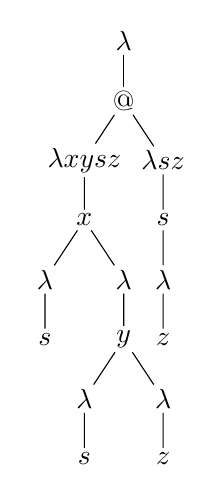
\begin{tikzpicture}[baseline=(root.base),level distance=5ex,inner ysep=0.5mm,sibling distance=10mm]
\node (root)
{$\lambda$}
child {node{$@$}
    child{node{$\lambda x y s z$}
        child { node{$x$}
            child{node{$\lambda$}{
                child {node {$s$}}}
            }
            child{node{$\lambda$}
                child{node{$y$}
                    child{node{$\lambda$}
                        child{ node {$s$}}
                    }
                    child{node{$\lambda$}
                        child{node{$z$}}}
                }
            }
        }
    }
    child{node{$\lambda s z$}
        child{node{$s$}
            child{node{$\lambda$} child{node{$z$}}}
        }
    }
}
;
\end{tikzpicture}

\begin{itemize}
\item Applying as many deterministic rules as possible gives the following traversal at which point the Opponent must make a choice:

$t_\epsilon = \Pstr[0.7cm]{(n0){\lambda }\ (n1){@}\ (n2-n1){\lambda x y s z}\ (n3-n2){x}\ (n4-n1){\lambda s z}\ (n5-n4){s}\ (n6-n3){\lambda }\ (n7-n2){s}\ (n8-n1){\ghostlmd^3}\ (n9-n0){\ghostvar^2} }$

(For readability we indicate the link label in exponent of the source node when representing traversals.)
The core of $t_\epsilon$ is
$\core{t_\epsilon} = \Pstr[0.7cm]{(n0){\lambda} \cdot (n9-n0){{\ghostvar^2}} }$
and therefore $\pview{\core{t_\epsilon}} =  \lambda\cdot \ghostvar^2$ is a path in  $\betanf{M}$.
This means that $\betanf{M}$ must be of the form $\lambda y s \ldots \cdot y N_1 \ldots \ldots N_q$ for some fresh variable $y$ and $s$ and $q\geq0$.

\item In order to determine what each argument $N_k$ is in the final normal form, we eta-expand by applying rule $\rulename{IVar}$ for each possible argument index $k\geq 1$ and then continue applying the traversal rules.

For $k=1$ we get the traversal:

$t_1 = \Pstr[0.7cm]{(n0){\lambda }\ (n1){@}\ (n2-n1){\lambda x y s z}\ (n3-n2){x}\ (n4-n1){\lambda s z}\
(n5-n4){s}\ (n6-n3){\lambda }\
(n7-n2){s}\ (n8-n1){\ghostlmd^3}\
(n9-n0){\ghostvar^2}
(n10-n9){\ghostlmd^1}
(n11-n8){\ghostvar^1}
(n12-n7){\ghostlmd^1}
(n13-n6){\ghostvar^1}
(n14-n5){\lambda^1}
(n15-n4)z
(n16-n3){\lambda^2}
(n17-n2)y
(n18-n1){\ghostlmd^2}
(n19-n0){\ghostvar^1}
}$

The P-view of the traversal core is
$\pview{\core{t_1}} = \Pstr[0.7cm]{(l){\lambda } \cdot (x-l){\ghostvar^2} \cdot (l1-x){\ghostlmd^1}
\cdot (x2-l){\ghostvar^1}
}$
which means that the normal form is of the form $\lambda y s \ldots \cdot s (y R_1 \ldots R_{q_2}) N_2 \ldots N_q$ for some terms $R_1$, \ldots $R_{q_2}$, and $q,q_2\geq 0$.

\item What should be the value of $q$? In other words, how many more $k$ do we need to look at?  The answer: we need to keep iterating on $k$ until the point where applying the traversal rules will only produce ghost variables and ghost lambda-nodes! Because there is a finite number of nodes in the computation tree, the variable node arities are bounded. Therefore for high enough index $k$, the eta-expansion case from rule \rulenamet{Var} will never be met:
        after applying rule \rulenamet{IVar} on $t_\epsilon$, all subsequent extensions of the traversal will be constructed using repeated applications of rule $\rulename{Lam^\ghostvar}$ or the eta-expanded case of rule $\rulename{Var}$.
     The upper-bound $q$ for $k$ is precisely given by the \emph{arity threshold} of the traversal $t_\epsilon$ as defined in~\ref{dfn:arity-threshold}.
     Here we have
     \begin{align*}
     \arth(t_\epsilon)
     = \max \{ & |s^2| , \\
               & |s^1| + (|s^2| - |\lambda|) , \\
               & |x| +  (|s^1| - |\lambda s z|) + (|s^2| - |\lambda|)
               %& |@| + (|x|- |\lambda x y s z |) + (|s^1| - |\lambda s z|) + (|s^2| -|\lambda|) \
               \} \\
    = \max \{   & 0 , \\
                & 1 + (0 - 0) , \\
                & 2 + (1 - 2) + (0 - 0)
                %& 2 + (2 - 4) + (1 - 2) + (0 - 0)
            \} \\
     = 1
     \end{align*}
     Thus we don't need to look at higher value of $k$ at $t_\epsilon$, we thus have:
     $\betanf{M} = \lambda y s \ldots \cdot s (y R_1 \ldots R_{q_2})$.

\item The arity threshold of $t_1$ is $\arth(t_1) = |z| + |y| - |\lambda^2| = 0+2-0 = 2$ hence  $\betanf{M}$ is of the form $\lambda y s \ldots \cdot s (y R_1 R_2)$.

\item Let's eta-expand using rule \rulenamet{IVar} for varying value of child index $1\leq k_2 \leq q_2 = 2$. We first look at the case $k_2 = 1$. The traversal obtained is:

$t_{11} = \Pstr[0.7cm]{
(n0){\lambda }\
(n1){@}\ (n2-n1){\lambda x y s z}\ (n3-n2){x}\ (n4-n1){\lambda s z}\ (n5-n4){s}\ (n6-n3){\lambda }\ (n7-n2){s}\ (n8-n1){\ghostlmd^3}\ (n9-n0){\ghostvar^2}
(n10-n9){\ghostlmd^1}
(n11-n8){\ghostvar^1}
(n12-n7){\ghostlmd^1}
(n13-n6){\ghostvar^1}
(n14-n5){\lambda^1}
(n15-n4)z
(n16-n3){\lambda^2}
(n17-n2)y
(n18-n1){\ghostlmd^2}
(n19-n0){\ghostvar^1}
(n20-n19){\ghostlmd^1}
(n21-n18){\ghostvar^1}
(n22-n17,60:1)\lambda % points to non-ghost node
(n23-n2,45:3) s
(n24-n1,45:3) {\ghostlmd^3}
(n25-n0,48:2) {\ghostvar^2}
}$

Thus $\pview{\core{t_{11}}} =
\Pstr[0.7cm]{
(n0){\lambda }\
 (n9-n0){\ghostvar^2}
 (n10-n9){\ghostlmd^1}
(n19-n0){\ghostvar^1}
(n20-n19){\ghostlmd^1}
(n25-n0,48:2){\ghostvar^2}
}$

Hence $\betanf{M}$ is of the form $\lambda y s \ldots \cdot s\ (y\ s\ R_2)$.

\item Now let's extend $t_1$ with \rulenamet{IVar^\lambda} for $k_2 = 2$. We get the traversal:

$t_{12} = \Pstr[0.7cm]{
(n0){\lambda }\
(n1){@}\ (n2-n1){\lambda x y s z}\
(n3-n2){x}\ (n4-n1){\lambda s z}\
(n5-n4){s}\
(n6-n3){\lambda }\
(n7-n2){s}\
(n8-n1){\ghostlmd^3}\
(n9-n0) {\ghostvar^2}
(n10-n9) {\ghostlmd^1}
(n11-n8){\ghostvar^1}
(n12-n7){\ghostlmd^1}
(n13-n6){\ghostvar^1}
(n14-n5)\lambda^1
(n15-n4)z
(n16-n3){\lambda^2}
(n17-n2)y
(n18-n1){\ghostlmd^2}
(n19-n0){\ghostvar^1}
(n20-n19){\ghostlmd^2} %%%%%%%%
(n21-n18){\ghostvar^2}
(n22-n17,60:2)\lambda % points to non-ghost node
(n23-n2,45:4) z
(n24-n1,45:4) {\ghostlmd^4}
(n25-n0,48:3) {\ghostvar^3}
}$

Thus $\pview{\core{t_{12}}} =
\Pstr[0.7cm]{
(n0){\lambda }\
 (n9-n0){{\ghostvar^2}}
 (n10-n9){\ghostlmd^1}
(n19-n0){\ghostvar^1}
(n20-n19){\ghostlmd^2}
(n25-n0,48:3) {\ghostvar^3}
}$

Hence $\betanf{M} = \lambda y s z \cdot s\ (y\ s\ z)$.
\end{itemize}
\end{example}

\begin{example}[``Missing operand'' example by Neil Jones]
\label{ex:missingoperand}
This small example illustrates how on-the-fly eta-expansion helps resolve the ``missing argument'' problem faced when using the traversal rules of STLC. Take $M = (\lambda u . u\ (y_1\ u)) (\lambda v . v\ y_2)$.

The computation tree is:
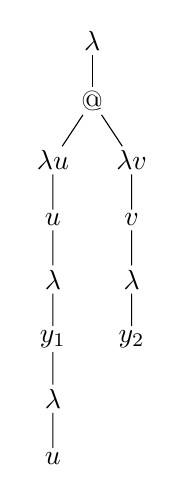
\begin{tikzpicture}[baseline=(root.base),level distance=5ex,inner ysep=0.5mm,sibling distance=10mm]
\node (root)
{$\lambda$}
child {node{$@$}
        child{node{$\lambda u $}
           child {node {$u$}
              child {node {$\lambda$}
                  child {node {$y_1$}
                      child {node {$\lambda$}
                          child {node {$u$}
                          }
                      }
                  }
              }
           }
        }
        child{node{$\lambda v$}
            child{node{$v$}
                child{node{$\lambda$}
                    child{ node {$y_2$}}
                }
            }
        }
    }
;
\end{tikzpicture}

The only two maximal normalizing traversals are:
\begin{itemize}

\item $t_1 = \Pstr[0.7cm]{(n0){\lambda }\ (n1){@}\ (n2-n1){\lambda u}\ (n3-n2){u}\ (n4-n1){\lambda v}\ (n5-n4){v}\ (n6-n3){\lambda }\ (n7-n0){y_1}\ (n8-n7){\lambda }\ (n9-n2){u}\ (n10-n1){\lambda v}\ (n11-n10){v}\ (n12-n9){{\ghostlmd^{1}}}\ (n13-n8){{\ghostvar^{1}}}\ (n14-n13){{\ghostlmd^{1}}}\ (n15-n12){{\ghostvar^{1}}}\ (n16-n11){\lambda }\ (n17-n0,35){y_2}\ }$
\item $t_2 = \Pstr[0.7cm]{(n0){\lambda }\ (n1){@}\ (n2-n1){\lambda u}\ (n3-n2){u}\ (n4-n1){\lambda v}\ (n5-n4){v}\ (n6-n3){\lambda }\ (n7-n0){y_1}\ (n8-n7){{\ghostlmd^{2}}}\ (n9-n6){{\ghostvar^{1}}}\ (n10-n5){\lambda }\ (n11-n0){y_2}\ }$
\end{itemize}
Using the STLC traversals, one can traverse $t_1$ all the way to variable $v$ at which point one get stuck due to the lack of operand applied to the last occurrence of $u$ (the occurrence  at the bottom of the left branch in the tree). Using ULC rule, that operands gets created on-the-fly through eta-expansion and is represented by ghost lambda node $\ghostlmd^1$.

The two core P-views give the two maximal paths in the beta-normal form of $M$:
\begin{itemize}
\item $\pview{\core{t_1}} = \Pstr[0.7cm]{(n0){\lambda }\ (n1-n0){y_1}\ (n2-n1){\lambda }\ (n3-n2){{\ghostvar^{1}}}\ (n4-n3){{\ghostlmd^{1}}}\ (n5-n0){y2}\ }$
\item $\pview{\core{t_2}} = \Pstr[0.7cm]{(n0){\lambda }\ (n1-n0){y_1}\ (n2-n1){{\ghostlmd^{2}}}\ (n3-n0){y_2}\ }$
\end{itemize}
Thus: $\betanf{M} = y_1 (\lambda  z.z\ y_2) y_2$.
\end{example}


\begin{example}[Neil Jones' ``$varity\ 2$'' example]

Take $M = varity\ two$ where
\begin{align*}
  varity &\equiv \lambda t.t (\lambda n a x . n (\lambda s z . a s (x s z))) (\lambda a. a) (\lambda z_0 . z_0) \\
  two &\equiv \lambda s_2 z_2 . s_2 (s_2\ z_2)
\end{align*}

In order to compute the set of normalizing traversals, we apply the traversal rules inductively until an input variable is reached, at which point we eta-expand with rule \rulenamet{IVar} for all possible values of $k$ ranging from $1$ to the arity threshold of the traversal. The first traversal obtained is denoted $t_\epsilon$, and for every sequence of integer $s \in \nat^*$,  the traversal $t_{s \cdot k}$ represents the maximal traversal obtained after extending $t_s$ using one application of the eta-expanded subcase of rule \rulenamet{IVar} with link-label $k \in \nat$.
This process yields the set of traversals $\{t_\epsilon, t_{11}, t_{12}, t_{121}, t_{122} \}$. Table~\ref{tab:varity2_trav_epsilon} represents $t_\epsilon$ and
Table~\ref{tab:varity2_trav} represents the three maximal traversals $t_{11}, t_{121}, t_{122}$.

\begin{table}
\resizebox{1.1\hsize}{!}{$
t_\epsilon = \Pstr[0.7cm]{(n0){\lambda }\ (n1){@}\ (n2-n1){\lambda t}\ (n3-n2){t}\ (n4-n1){\lambda s_2 z_2}\ (n5-n4){s_2}\ (n6-n3){\lambda n a x}\ (n7-n6){n}\ (n8-n5){\lambda }\ (n9-n4){s_2}\ (n10-n3){\lambda n a x}\ (n11-n10){n}\ (n12-n9){\lambda }\ (n13-n4){z_2}\ (n14-n3){\lambda a}\ (n15-n14){a}\ (n16-n13){{\ghostlmd^{1}}}\ (n17-n12){{\ghostvar^{1}}}\ (n18-n11){\lambda s z}\ (n19-n10){a}\ (n20-n9){{\ghostlmd^{2}}}\ (n21-n8){{\ghostvar^{1}}}\ (n22-n7){\lambda s z}\ (n23-n6){a}\ (n24-n5){{\ghostlmd^{2}}}\ (n25-n4){{\ghostvar^{3}}}\
(n26-n3){\lambda z_0}\ (n27-n26){z_0}\ (n28-n25){{\ghostlmd^{1}}}\ (n29-n24){{\ghostvar^{1}}}\
(n30-n23){\lambda }\ (n31-n22){s}\ (n32-n21){{\ghostlmd^{1}}}\ (n33-n20){{\ghostvar^{1}}}\ (n34-n19){\lambda }\ (n35-n18){s}\ (n36-n17){{\ghostlmd^{1}}}\ (n37-n16){{\ghostvar^{1}}}\ (n38-n15){{\ghostlmd^{1}}}\ (n39-n14){{\ghostvar^{2}}}\ (n40-n13){{\ghostlmd^{2}}}\ (n41-n12){{\ghostvar^{2}}}\ (n42-n11){{\ghostlmd^{2}}}\ (n43-n10){{\ghostvar^{4}}}\ (n44-n9){{\ghostlmd^{4}}}\ (n45-n8){{\ghostvar^{3}}}\ (n46-n7){{\ghostlmd^{3}}}\ (n47-n6){{\ghostvar^{5}}}\ (n48-n5){{\ghostlmd^{5}}}\ (n49-n4){{\ghostvar^{6}}}\ (n50-n3){{\ghostlmd^{6}}}\ (n51-n2){{\ghostvar^{4}}}\ (n52-n1){{\ghostlmd^{4}}}\ (n53-n0){{\ghostvar^{3}}}}$}
\caption{Traversal $t_\epsilon$ of $varity\ 2$}
\label{tab:varity2_trav_epsilon}
\end{table}

\newgeometry{left=1cm,right=2cm, bottom=2cm, top=2cm}
\begin{landscape}
\thispagestyle{empty}
\begin{table}
% \resizebox{1.1\hsize}{!}{$t_{1} = \Pstr[0.7cm]{(n0){\lambda }\ (n1){@}\ (n2-n1){\lambda t}\ (n3-n2){t}\ (n4-n1){\lambda s_2 z_2}\ (n5-n4){s_2}\ (n6-n3){\lambda n a x}\ (n7-n6){n}\ (n8-n5){\lambda}\ (n9-n4){s_2}\ (n10-n3){\lambda n a x}\ (n11-n10){n}\ (n12-n9){\lambda}\ (n13-n4){z_2}\ (n14-n3){\lambda a}\ (n15-n14){a}\ (n16-n13){{\ghostlmd^{1}}}\ (n17-n12){{\ghostvar^{1}}}\ (n18-n11){\lambda s z}\ (n19-n10){a}\ (n20-n9){{\ghostlmd^{2}}}\ (n21-n8){{\ghostvar^{1}}}\ (n22-n7){\lambda s z}\ (n23-n6){a}\ (n24-n5){{\ghostlmd^{2}}}\ (n25-n4){{\ghostvar^{3}}}\ (n26-n3){\lambda z_0}\ (n27-n26){z_0}\ (n28-n25){{\ghostlmd^{1}}}\ (n29-n24){{\ghostvar^{1}}}\ (n30-n23){\lambda }\ (n31-n22){s}\ (n32-n21){{\ghostlmd^{1}}}\ (n33-n20){{\ghostvar^{1}}}\ (n34-n19){\lambda }\ (n35-n18){s}\ (n36-n17){{\ghostlmd^{1}}}\ (n37-n16){{\ghostvar^{1}}}\ (n38-n15){{\ghostlmd^{1}}}\ (n39-n14){{\ghostvar^{2}}}\ (n40-n13){{\ghostlmd^{2}}}\ (n41-n12){{\ghostvar^{2}}}\ (n42-n11){{\ghostlmd^{2}}}\ (n43-n10){{\ghostvar^{4}}}\ (n44-n9){{\ghostlmd^{4}}}\ (n45-n8){{\ghostvar^{3}}}\ (n46-n7){{\ghostlmd^{3}}}\ (n47-n6){{\ghostvar^{5}}}\ (n48-n5){{\ghostlmd^{5}}}\ (n49-n4){{\ghostvar^{6}}}\ (n50-n3){{\ghostlmd^{6}}}\ (n51-n2){{\ghostvar^{4}}}\ (n52-n1){{\ghostlmd^{4}}}\ (n53-n0){{\ghostvar^{3}}}\ (n54-n53){{\ghostlmd^{1}}}\ (n55-n52){{\ghostvar^{1}}}\ (n56-n51){{\ghostlmd^{1}}}\ (n57-n50){{\ghostvar^{1}}}\ (n58-n49){{\ghostlmd^{1}}}\ (n59-n48){{\ghostvar^{1}}}\ (n60-n47){{\ghostlmd^{1}}}\ (n61-n46){{\ghostvar^{1}}}\ (n62-n45){{\ghostlmd^{1}}}\ (n63-n44){{\ghostvar^{1}}}\ (n64-n43){{\ghostlmd^{1}}}\ (n65-n42){{\ghostvar^{1}}}\ (n66-n41){{\ghostlmd^{1}}}\ (n67-n40){{\ghostvar^{1}}}\ (n68-n39){{\ghostlmd^{1}}}\ (n69-n38){{\ghostvar^{1}}}\ (n70-n37){{\ghostlmd^{1}}}\ (n71-n36){{\ghostvar^{1}}}\ (n72-n35){{\ghostlmd^{1}}}\ (n73-n34){{\ghostvar^{1}}}\ (n74-n33){{\ghostlmd^{1}}}\ (n75-n32){{\ghostvar^{1}}}\ (n76-n31){{\ghostlmd^{1}}}\ (n77-n30){{\ghostvar^{1}}}\ (n78-n29){{\ghostlmd^{1}}}\ (n79-n28){{\ghostvar^{1}}}\ (n80-n27){{\ghostlmd^{1}}}\ (n81-n26){{\ghostvar^{2}}}\ (n82-n25){{\ghostlmd^{2}}}\ (n83-n24){{\ghostvar^{2}}}\ (n84-n23){\lambda }\ (n85-n6){x}\ (n86-n5){{\ghostlmd^{3}}}\ (n87-n4){{\ghostvar^{4}}}\ (n88-n3){{\ghostlmd^{4}}}\ (n89-n2){{\ghostvar^{2}}}\ (n90-n1){{\ghostlmd^{2}}}\ (n91-n0){{\ghostvar^{1}}}}$}
\resizebox{1\hsize}{!}{$t_{11} = \Pstr[0.7cm]{(n0){\lambda }\ (n1){@}\ (n2-n1){\lambda t}\ (n3-n2){t}\ (n4-n1){\lambda s_2 z_2}\ (n5-n4){s_2}\ (n6-n3){\lambda n a x}\ (n7-n6){n}\ (n8-n5){\lambda }\ (n9-n4){s_2}\ (n10-n3){\lambda n a x}\ (n11-n10){n}\ (n12-n9){\lambda }\ (n13-n4){z_2}\ (n14-n3){\lambda a}\ (n15-n14){a}\ (n16-n13){{\ghostlmd^{1}}}\ (n17-n12){{\ghostvar^{1}}}\ (n18-n11){\lambda s z}\ (n19-n10){a}\ (n20-n9){{\ghostlmd^{2}}}\ (n21-n8){{\ghostvar^{1}}}\ (n22-n7){\lambda s z}\ (n23-n6){a}\ (n24-n5){{\ghostlmd^{2}}}\ (n25-n4){{\ghostvar^{3}}}\ (n26-n3){\lambda z_0}\ (n27-n26){z_0}\ (n28-n25){{\ghostlmd^{1}}}\ (n29-n24){{\ghostvar^{1}}}\ (n30-n23){\lambda }\ (n31-n22){s}\ (n32-n21){{\ghostlmd^{1}}}\ (n33-n20){{\ghostvar^{1}}}\ (n34-n19){\lambda }\ (n35-n18){s}\ (n36-n17){{\ghostlmd^{1}}}\ (n37-n16){{\ghostvar^{1}}}\ (n38-n15){{\ghostlmd^{1}}}\ (n39-n14){{\ghostvar^{2}}}\ (n40-n13){{\ghostlmd^{2}}}\ (n41-n12){{\ghostvar^{2}}}\ (n42-n11){{\ghostlmd^{2}}}\ (n43-n10){{\ghostvar^{4}}}\ (n44-n9){{\ghostlmd^{4}}}\ (n45-n8){{\ghostvar^{3}}}\ (n46-n7){{\ghostlmd^{3}}}\ (n47-n6){{\ghostvar^{5}}}\ (n48-n5){{\ghostlmd^{5}}}\ (n49-n4){{\ghostvar^{6}}}\ (n50-n3){{\ghostlmd^{6}}}\ (n51-n2){{\ghostvar^{4}}}\ (n52-n1){{\ghostlmd^{4}}}\ (n53-n0){{\ghostvar^{3}}}\ (n54-n53){{\ghostlmd^{1}}}\ (n55-n52){{\ghostvar^{1}}}\ (n56-n51){{\ghostlmd^{1}}}\ (n57-n50){{\ghostvar^{1}}}\ (n58-n49){{\ghostlmd^{1}}}\ (n59-n48){{\ghostvar^{1}}}\ (n60-n47){{\ghostlmd^{1}}}\ (n61-n46){{\ghostvar^{1}}}\ (n62-n45){{\ghostlmd^{1}}}\ (n63-n44){{\ghostvar^{1}}}\ (n64-n43){{\ghostlmd^{1}}}\ (n65-n42){{\ghostvar^{1}}}\ (n66-n41){{\ghostlmd^{1}}}\ (n67-n40){{\ghostvar^{1}}}\ (n68-n39){{\ghostlmd^{1}}}\ (n69-n38){{\ghostvar^{1}}}\ (n70-n37){{\ghostlmd^{1}}}\ (n71-n36){{\ghostvar^{1}}}\ (n72-n35){{\ghostlmd^{1}}}\ (n73-n34){{\ghostvar^{1}}}\ (n74-n33){{\ghostlmd^{1}}}\ (n75-n32){{\ghostvar^{1}}}\ (n76-n31){{\ghostlmd^{1}}}\ (n77-n30){{\ghostvar^{1}}}\ (n78-n29){{\ghostlmd^{1}}}\ (n79-n28){{\ghostvar^{1}}}\ (n80-n27){{\ghostlmd^{1}}}\ (n81-n26){{\ghostvar^{2}}}\ (n82-n25){{\ghostlmd^{2}}}\ (n83-n24){{\ghostvar^{2}}}\ (n84-n23){\lambda }\ (n85-n6){x}\ (n86-n5){{\ghostlmd^{3}}}\ (n87-n4){{\ghostvar^{4}}}\ (n88-n3){{\ghostlmd^{4}}}\ (n89-n2){{\ghostvar^{2}}}\ (n90-n1){{\ghostlmd^{2}}}\ (n91-n0){{\ghostvar^{1}}}\ (n92-n91){{\ghostlmd^{1}}}\ (n93-n90){{\ghostvar^{1}}}\ (n94-n89){{\ghostlmd^{1}}}\ (n95-n88){{\ghostvar^{1}}}\ (n96-n87){{\ghostlmd^{1}}}\ (n97-n86){{\ghostvar^{1}}}\ (n98-n85){\lambda }\ (n99-n22){s}\ (n100-n21){{\ghostlmd^{1}}}\ (n101-n20){{\ghostvar^{1}}}\ (n102-n19){\lambda }\ (n103-n18){s}\ (n104-n17){{\ghostlmd^{1}}}\ (n105-n16){{\ghostvar^{1}}}\ (n106-n15){{\ghostlmd^{1}}}\ (n107-n14){{\ghostvar^{2}}}\ (n108-n13){{\ghostlmd^{2}}}\ (n109-n12){{\ghostvar^{2}}}\ (n110-n11){{\ghostlmd^{2}}}\ (n111-n10){{\ghostvar^{4}}}\ (n112-n9){{\ghostlmd^{4}}}\ (n113-n8){{\ghostvar^{3}}}\ (n114-n7){{\ghostlmd^{3}}}\ (n115-n6){{\ghostvar^{5}}}\ (n116-n5){{\ghostlmd^{5}}}\ (n117-n4){{\ghostvar^{6}}}\ (n118-n3){{\ghostlmd^{6}}}\ (n119-n2){{\ghostvar^{4}}}\ (n120-n1){{\ghostlmd^{4}}}\ (n121-n0){{\ghostvar^{3}}}}$}
% \resizebox{1.1\hsize}{!}{$t_{12} = \Pstr[0.7cm]{(n0){\lambda }\ (n1){@}\ (n2-n1){\lambda t}\ (n3-n2){t}\ (n4-n1){\lambda s_2 z_2}\ (n5-n4){s_2}\ (n6-n3){\lambda n a x}\ (n7-n6){n}\ (n8-n5){\lambda }\ (n9-n4){s_2}\ (n10-n3){\lambda n a x}\ (n11-n10){n}\ (n12-n9){\lambda }\ (n13-n4){z_2}\ (n14-n3){\lambda a}\ (n15-n14){a}\ (n16-n13){{\ghostlmd^{1}}}\ (n17-n12){{\ghostvar^{1}}}\ (n18-n11){\lambda s z}\ (n19-n10){a}\ (n20-n9){{\ghostlmd^{2}}}\ (n21-n8){{\ghostvar^{1}}}\ (n22-n7){\lambda s z}\ (n23-n6){a}\ (n24-n5){{\ghostlmd^{2}}}\ (n25-n4){{\ghostvar^{3}}}\ (n26-n3){\lambda z_0}\ (n27-n26){z_0}\ (n28-n25){{\ghostlmd^{1}}}\ (n29-n24){{\ghostvar^{1}}}\ (n30-n23){\lambda }\ (n31-n22){s}\ (n32-n21){{\ghostlmd^{1}}}\ (n33-n20){{\ghostvar^{1}}}\ (n34-n19){\lambda }\ (n35-n18){s}\ (n36-n17){{\ghostlmd^{1}}}\ (n37-n16){{\ghostvar^{1}}}\ (n38-n15){{\ghostlmd^{1}}}\ (n39-n14){{\ghostvar^{2}}}\ (n40-n13){{\ghostlmd^{2}}}\ (n41-n12){{\ghostvar^{2}}}\ (n42-n11){{\ghostlmd^{2}}}\ (n43-n10){{\ghostvar^{4}}}\ (n44-n9){{\ghostlmd^{4}}}\ (n45-n8){{\ghostvar^{3}}}\ (n46-n7){{\ghostlmd^{3}}}\ (n47-n6){{\ghostvar^{5}}}\ (n48-n5){{\ghostlmd^{5}}}\ (n49-n4){{\ghostvar^{6}}}\ (n50-n3){{\ghostlmd^{6}}}\ (n51-n2){{\ghostvar^{4}}}\ (n52-n1){{\ghostlmd^{4}}}\ (n53-n0){{\ghostvar^{3}}}\ (n54-n53){{\ghostlmd^{1}}}\ (n55-n52){{\ghostvar^{1}}}\ (n56-n51){{\ghostlmd^{1}}}\ (n57-n50){{\ghostvar^{1}}}\ (n58-n49){{\ghostlmd^{1}}}\ (n59-n48){{\ghostvar^{1}}}\ (n60-n47){{\ghostlmd^{1}}}\ (n61-n46){{\ghostvar^{1}}}\ (n62-n45){{\ghostlmd^{1}}}\ (n63-n44){{\ghostvar^{1}}}\ (n64-n43){{\ghostlmd^{1}}}\ (n65-n42){{\ghostvar^{1}}}\ (n66-n41){{\ghostlmd^{1}}}\ (n67-n40){{\ghostvar^{1}}}\ (n68-n39){{\ghostlmd^{1}}}\ (n69-n38){{\ghostvar^{1}}}\ (n70-n37){{\ghostlmd^{1}}}\ (n71-n36){{\ghostvar^{1}}}\ (n72-n35){{\ghostlmd^{1}}}\ (n73-n34){{\ghostvar^{1}}}\ (n74-n33){{\ghostlmd^{1}}}\ (n75-n32){{\ghostvar^{1}}}\ (n76-n31){{\ghostlmd^{1}}}\ (n77-n30){{\ghostvar^{1}}}\ (n78-n29){{\ghostlmd^{1}}}\ (n79-n28){{\ghostvar^{1}}}\ (n80-n27){{\ghostlmd^{1}}}\ (n81-n26){{\ghostvar^{2}}}\ (n82-n25){{\ghostlmd^{2}}}\ (n83-n24){{\ghostvar^{2}}}\ (n84-n23){\lambda }\ (n85-n6){x}\ (n86-n5){{\ghostlmd^{3}}}\ (n87-n4){{\ghostvar^{4}}}\ (n88-n3){{\ghostlmd^{4}}}\ (n89-n2){{\ghostvar^{2}}}\ (n90-n1){{\ghostlmd^{2}}}\ (n91-n0){{\ghostvar^{1}}}\ (n92-n91){{\ghostlmd^{2}}}\ (n93-n90){{\ghostvar^{2}}}\ (n94-n89){{\ghostlmd^{2}}}\ (n95-n88){{\ghostvar^{2}}}\ (n96-n87){{\ghostlmd^{2}}}\ (n97-n86){{\ghostvar^{2}}}\ (n98-n85){\lambda }\ (n99-n22){z}\ (n100-n21){{\ghostlmd^{2}}}\ (n101-n20){{\ghostvar^{2}}}\ (n102-n19){\lambda }\ (n103-n10){x}\ (n104-n9){{\ghostlmd^{3}}}\ (n105-n8){{\ghostvar^{2}}}\ (n106-n7){{\ghostlmd^{2}}}\ (n107-n6){{\ghostvar^{4}}}\ (n108-n5){{\ghostlmd^{4}}}\ (n109-n4){{\ghostvar^{5}}}\ (n110-n3){{\ghostlmd^{5}}}\ (n111-n2){{\ghostvar^{3}}}\ (n112-n1){{\ghostlmd^{3}}}\ (n113-n0){{\ghostvar^{2}}}}$}
\resizebox{1\hsize}{!}{$t_{121} =
\Pstr[0.7cm]{(n0){\lambda }\ (n1){@}\ (n2-n1){\lambda t}\ (n3-n2){t}\ (n4-n1){\lambda s_2 z_2}\ (n5-n4){s_2}\ (n6-n3){\lambda n a x}\ (n7-n6){n}\ (n8-n5){\lambda }\ (n9-n4){s_2}\ (n10-n3){\lambda n a x}\ (n11-n10){n}\ (n12-n9){\lambda }\ (n13-n4){z_2}\ (n14-n3){\lambda a}\ (n15-n14){a}\ (n16-n13){{\ghostlmd^{1}}}\ (n17-n12){{\ghostvar^{1}}}\ (n18-n11){\lambda s z}\ (n19-n10){a}\ (n20-n9){{\ghostlmd^{2}}}\ (n21-n8){{\ghostvar^{1}}}\ (n22-n7){\lambda s z}\ (n23-n6){a}\ (n24-n5){{\ghostlmd^{2}}}\ (n25-n4){{\ghostvar^{3}}}\ (n26-n3){\lambda z_0}\ (n27-n26){z_0}\ (n28-n25){{\ghostlmd^{1}}}\ (n29-n24){{\ghostvar^{1}}}\ (n30-n23){\lambda }\ (n31-n22){s}\ (n32-n21){{\ghostlmd^{1}}}\ (n33-n20){{\ghostvar^{1}}}\ (n34-n19){\lambda }\ (n35-n18){s}\ (n36-n17){{\ghostlmd^{1}}}\ (n37-n16){{\ghostvar^{1}}}\ (n38-n15){{\ghostlmd^{1}}}\ (n39-n14){{\ghostvar^{2}}}\ (n40-n13){{\ghostlmd^{2}}}\ (n41-n12){{\ghostvar^{2}}}\ (n42-n11){{\ghostlmd^{2}}}\ (n43-n10){{\ghostvar^{4}}}\ (n44-n9){{\ghostlmd^{4}}}\ (n45-n8){{\ghostvar^{3}}}\ (n46-n7){{\ghostlmd^{3}}}\ (n47-n6){{\ghostvar^{5}}}\ (n48-n5){{\ghostlmd^{5}}}\ (n49-n4){{\ghostvar^{6}}}\ (n50-n3){{\ghostlmd^{6}}}\ (n51-n2){{\ghostvar^{4}}}\ (n52-n1){{\ghostlmd^{4}}}\ (n53-n0){{\ghostvar^{3}}}\ (n54-n53){{\ghostlmd^{1}}}\ (n55-n52){{\ghostvar^{1}}}\ (n56-n51){{\ghostlmd^{1}}}\ (n57-n50){{\ghostvar^{1}}}\ (n58-n49){{\ghostlmd^{1}}}\ (n59-n48){{\ghostvar^{1}}}\ (n60-n47){{\ghostlmd^{1}}}\ (n61-n46){{\ghostvar^{1}}}\ (n62-n45){{\ghostlmd^{1}}}\ (n63-n44){{\ghostvar^{1}}}\ (n64-n43){{\ghostlmd^{1}}}\ (n65-n42){{\ghostvar^{1}}}\ (n66-n41){{\ghostlmd^{1}}}\ (n67-n40){{\ghostvar^{1}}}\ (n68-n39){{\ghostlmd^{1}}}\ (n69-n38){{\ghostvar^{1}}}\ (n70-n37){{\ghostlmd^{1}}}\ (n71-n36){{\ghostvar^{1}}}\ (n72-n35){{\ghostlmd^{1}}}\ (n73-n34){{\ghostvar^{1}}}\ (n74-n33){{\ghostlmd^{1}}}\ (n75-n32){{\ghostvar^{1}}}\ (n76-n31){{\ghostlmd^{1}}}\ (n77-n30){{\ghostvar^{1}}}\ (n78-n29){{\ghostlmd^{1}}}\ (n79-n28){{\ghostvar^{1}}}\ (n80-n27){{\ghostlmd^{1}}}\ (n81-n26){{\ghostvar^{2}}}\ (n82-n25){{\ghostlmd^{2}}}\ (n83-n24){{\ghostvar^{2}}}\ (n84-n23){\lambda }\ (n85-n6){x}\ (n86-n5){{\ghostlmd^{3}}}\ (n87-n4){{\ghostvar^{4}}}\ (n88-n3){{\ghostlmd^{4}}}\ (n89-n2){{\ghostvar^{2}}}\ (n90-n1){{\ghostlmd^{2}}}\ (n91-n0){{\ghostvar^{1}}}\ (n92-n91){{\ghostlmd^{2}}}\ (n93-n90){{\ghostvar^{2}}}\ (n94-n89){{\ghostlmd^{2}}}\ (n95-n88){{\ghostvar^{2}}}\ (n96-n87){{\ghostlmd^{2}}}\ (n97-n86){{\ghostvar^{2}}}\ (n98-n85){\lambda }\ (n99-n22){z}\ (n100-n21){{\ghostlmd^{2}}}\ (n101-n20){{\ghostvar^{2}}}\ (n102-n19){\lambda }\ (n103-n10){x}\ (n104-n9){{\ghostlmd^{3}}}\ (n105-n8){{\ghostvar^{2}}}\ (n106-n7){{\ghostlmd^{2}}}\ (n107-n6){{\ghostvar^{4}}}\ (n108-n5){{\ghostlmd^{4}}}\ (n109-n4){{\ghostvar^{5}}}\ (n110-n3){{\ghostlmd^{5}}}\ (n111-n2){{\ghostvar^{3}}}\ (n112-n1){{\ghostlmd^{3}}}\ (n113-n0){{\ghostvar^{2}}}\ (n114-n113){{\ghostlmd^{1}}}\ (n115-n112){{\ghostvar^{1}}}\ (n116-n111){{\ghostlmd^{1}}}\ (n117-n110){{\ghostvar^{1}}}\ (n118-n109){{\ghostlmd^{1}}}\ (n119-n108){{\ghostvar^{1}}}\ (n120-n107){{\ghostlmd^{1}}}\ (n121-n106){{\ghostvar^{1}}}\ (n122-n105){{\ghostlmd^{1}}}\ (n123-n104){{\ghostvar^{1}}}\ (n124-n103){\lambda }\ (n125-n18){s}\ (n126-n17){{\ghostlmd^{1}}}\ (n127-n16){{\ghostvar^{1}}}\ (n128-n15){{\ghostlmd^{1}}}\ (n129-n14){{\ghostvar^{2}}}\ (n130-n13){{\ghostlmd^{2}}}\ (n131-n12){{\ghostvar^{2}}}\ (n132-n11){{\ghostlmd^{2}}}\ (n133-n10){{\ghostvar^{4}}}\ (n134-n9){{\ghostlmd^{4}}}\ (n135-n8){{\ghostvar^{3}}}\ (n136-n7){{\ghostlmd^{3}}}\ (n137-n6){{\ghostvar^{5}}}\ (n138-n5){{\ghostlmd^{5}}}\ (n139-n4){{\ghostvar^{6}}}\ (n140-n3){{\ghostlmd^{6}}}\ (n141-n2){{\ghostvar^{4}}}\ (n142-n1){{\ghostlmd^{4}}}\ (n143-n0){{\ghostvar^{3}}}}$}

\resizebox{1\hsize}{!}{$t_{122} =
\Pstr[0.7cm]{(n0){\lambda }\ (n1){@}\ (n2-n1){\lambda t}\ (n3-n2){t}\ (n4-n1){\lambda s_2 z_2}\ (n5-n4){s_2}\ (n6-n3){\lambda n a x}\ (n7-n6){n}\ (n8-n5){\lambda }\ (n9-n4){s_2}\ (n10-n3){\lambda n a x}\ (n11-n10){n}\ (n12-n9){\lambda }\ (n13-n4){z_2}\ (n14-n3){\lambda a}\ (n15-n14){a}\ (n16-n13){{\ghostlmd^{1}}}\ (n17-n12){{\ghostvar^{1}}}\ (n18-n11){\lambda s z}\ (n19-n10){a}\ (n20-n9){{\ghostlmd^{2}}}\ (n21-n8){{\ghostvar^{1}}}\ (n22-n7){\lambda s z}\ (n23-n6){a}\ (n24-n5){{\ghostlmd^{2}}}\ (n25-n4){{\ghostvar^{3}}}\ (n26-n3){\lambda z_0}\ (n27-n26){z_0}\ (n28-n25){{\ghostlmd^{1}}}\ (n29-n24){{\ghostvar^{1}}}\ (n30-n23){\lambda }\ (n31-n22){s}\ (n32-n21){{\ghostlmd^{1}}}\ (n33-n20){{\ghostvar^{1}}}\ (n34-n19){\lambda }\ (n35-n18){s}\ (n36-n17){{\ghostlmd^{1}}}\ (n37-n16){{\ghostvar^{1}}}\ (n38-n15){{\ghostlmd^{1}}}\ (n39-n14){{\ghostvar^{2}}}\ (n40-n13){{\ghostlmd^{2}}}\ (n41-n12){{\ghostvar^{2}}}\ (n42-n11){{\ghostlmd^{2}}}\ (n43-n10){{\ghostvar^{4}}}\ (n44-n9){{\ghostlmd^{4}}}\ (n45-n8){{\ghostvar^{3}}}\ (n46-n7){{\ghostlmd^{3}}}\ (n47-n6){{\ghostvar^{5}}}\ (n48-n5){{\ghostlmd^{5}}}\ (n49-n4){{\ghostvar^{6}}}\ (n50-n3){{\ghostlmd^{6}}}\ (n51-n2){{\ghostvar^{4}}}\ (n52-n1){{\ghostlmd^{4}}}\ (n53-n0){{\ghostvar^{3}}}\ (n54-n53){{\ghostlmd^{1}}}\ (n55-n52){{\ghostvar^{1}}}\ (n56-n51){{\ghostlmd^{1}}}\ (n57-n50){{\ghostvar^{1}}}\ (n58-n49){{\ghostlmd^{1}}}\ (n59-n48){{\ghostvar^{1}}}\ (n60-n47){{\ghostlmd^{1}}}\ (n61-n46){{\ghostvar^{1}}}\ (n62-n45){{\ghostlmd^{1}}}\ (n63-n44){{\ghostvar^{1}}}\ (n64-n43){{\ghostlmd^{1}}}\ (n65-n42){{\ghostvar^{1}}}\ (n66-n41){{\ghostlmd^{1}}}\ (n67-n40){{\ghostvar^{1}}}\ (n68-n39){{\ghostlmd^{1}}}\ (n69-n38){{\ghostvar^{1}}}\ (n70-n37){{\ghostlmd^{1}}}\ (n71-n36){{\ghostvar^{1}}}\ (n72-n35){{\ghostlmd^{1}}}\ (n73-n34){{\ghostvar^{1}}}\ (n74-n33){{\ghostlmd^{1}}}\ (n75-n32){{\ghostvar^{1}}}\ (n76-n31){{\ghostlmd^{1}}}\ (n77-n30){{\ghostvar^{1}}}\ (n78-n29){{\ghostlmd^{1}}}\ (n79-n28){{\ghostvar^{1}}}\ (n80-n27){{\ghostlmd^{1}}}\ (n81-n26){{\ghostvar^{2}}}\ (n82-n25){{\ghostlmd^{2}}}\ (n83-n24){{\ghostvar^{2}}}\ (n84-n23){\lambda }\ (n85-n6){x}\ (n86-n5){{\ghostlmd^{3}}}\ (n87-n4){{\ghostvar^{4}}}\ (n88-n3){{\ghostlmd^{4}}}\ (n89-n2){{\ghostvar^{2}}}\ (n90-n1){{\ghostlmd^{2}}}\ (n91-n0){{\ghostvar^{1}}}\ (n92-n91){{\ghostlmd^{2}}}\ (n93-n90){{\ghostvar^{2}}}\ (n94-n89){{\ghostlmd^{2}}}\ (n95-n88){{\ghostvar^{2}}}\ (n96-n87){{\ghostlmd^{2}}}\ (n97-n86){{\ghostvar^{2}}}\ (n98-n85){\lambda }\ (n99-n22){z}\ (n100-n21){{\ghostlmd^{2}}}\ (n101-n20){{\ghostvar^{2}}}\ (n102-n19){\lambda }\ (n103-n10){x}\ (n104-n9){{\ghostlmd^{3}}}\ (n105-n8){{\ghostvar^{2}}}\ (n106-n7){{\ghostlmd^{2}}}\ (n107-n6){{\ghostvar^{4}}}\ (n108-n5){{\ghostlmd^{4}}}\ (n109-n4){{\ghostvar^{5}}}\ (n110-n3){{\ghostlmd^{5}}}\ (n111-n2){{\ghostvar^{3}}}\ (n112-n1){{\ghostlmd^{3}}}\ (n113-n0){{\ghostvar^{2}}}\ (n114-n113){{\ghostlmd^{2}}}\ (n115-n112){{\ghostvar^{2}}}\ (n116-n111){{\ghostlmd^{2}}}\ (n117-n110){{\ghostvar^{2}}}\ (n118-n109){{\ghostlmd^{2}}}\ (n119-n108){{\ghostvar^{2}}}\ (n120-n107){{\ghostlmd^{2}}}\ (n121-n106){{\ghostvar^{2}}}\ (n122-n105){{\ghostlmd^{2}}}\ (n123-n104){{\ghostvar^{2}}}\ (n124-n103){\lambda }\ (n125-n18){z}\ (n126-n17){{\ghostlmd^{2}}}\ (n127-n16){{\ghostvar^{2}}}\ (n128-n15){{\ghostlmd^{2}}}\ (n129-n14){{\ghostvar^{3}}}\ (n130-n13){{\ghostlmd^{3}}}\ (n131-n12){{\ghostvar^{3}}}\ (n132-n11){{\ghostlmd^{3}}}\ (n133-n10){{\ghostvar^{5}}}\ (n134-n9){{\ghostlmd^{5}}}\ (n135-n8){{\ghostvar^{4}}}\ (n136-n7){{\ghostlmd^{4}}}\ (n137-n6){{\ghostvar^{6}}}\ (n138-n5){{\ghostlmd^{6}}}\ (n139-n4){{\ghostvar^{7}}}\ (n140-n3){{\ghostlmd^{7}}}\ (n141-n2){{\ghostvar^{5}}}\ (n142-n1){{\ghostlmd^{5}}}\ (n143-n0){{\ghostvar^{4}}}}$}
\caption{Maximal traversals of $varity\ 2$}
\label{tab:varity2_trav}
\end{table}
\end{landscape}
\restoregeometry

Keeping only the maximal traversals gives us the following set of maximal normalizing traversals of $M$:
$$\travsetnorm_{\max}(M) = \{ t_{11}, t_{121}, t_{122} \}$$

Hence the set of maximal paths in the beta-normal form of $M$ is given by the traversal core P-views:
\begin{align*}
\pview{\core{t_{11}}} &=
    \Pstr[0.7cm]{(n0){\lambda }\ (n1-n0){{\ghostvar^{3}}}\ (n2-n1){{\ghostlmd^{1}}}\ (n3-n0){{\ghostvar^{1}}}\ (n4-n3){{\ghostlmd^{1}}}\ (n5-n0){{\ghostvar^{3}}}}
\\
\pview{\core{t_{121}}} &=
    \Pstr[0.7cm]{(n0){\lambda }\ (n1-n0){{\ghostvar^{3}}}\ (n2-n1){{\ghostlmd^{1}}}\ (n3-n0){{\ghostvar^{1}}}\ (n4-n3){{\ghostlmd^{2}}}\ (n5-n0){{\ghostvar^{2}}}\ (n6-n5){{\ghostlmd^{1}}}\ (n7-n0){{\ghostvar^{3}}}}
\\
\pview{\core{t_{122}}} &=
\Pstr[0.7cm]{(n0){\lambda }\ (n1-n0){{\ghostvar^{3}}}\ (n2-n1){{\ghostlmd^{1}}}\ (n3-n0){{\ghostvar^{1}}}\ (n4-n3){{\ghostlmd^{2}}}\ (n5-n0){{\ghostvar^{2}}}\ (n6-n5){{\ghostlmd^{2}}}\ (n7-n0){{\ghostvar^{4}}}}
\end{align*}

Therefore the beta-normal from of $varity\ 2$ is:
\begin{align*}
\betanf{varity\ 2} &= \lambda x_1 x_2 x_3 x_4 . x_3 (x_1 x_3 (x_2 x_3 x_4))\\
&\equiv_\alpha \lambda x y s z . s (x s (y s z))
\end{align*}
\end{example}

\begin{example}
Take the fixed-point combinator $\Omega = (\lambda x. x x) (\lambda y. y y)$ with computation tree:
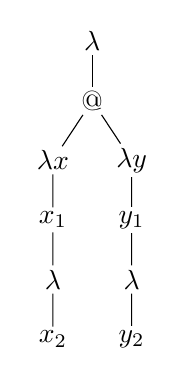
\begin{tikzpicture}[baseline=(root.base),level distance=5ex,inner ysep=0.5mm,sibling distance=10mm]
    \node (root)
    {$\lambda$}
    child {node{$@$}
            child{node{$\lambda x $}
               child {node {$x_1$}
                  child {node {$\lambda$}
                      child {node {$x_2$}
                      }
                  }
               }
            }
            child{node{$\lambda y$}
                child{node{$y_1$}
                    child{node{$\lambda$}
                        child{ node {$y_2$}}
                    }
                }
            }
        }
    ;
\end{tikzpicture}
It's a well known fact that $\Omega$ does not have a normal form.
The term has a unique (infinite) traversal starting with
$\Pstr[0.7cm]{{\lambda}\ (n1){@}\ (n2-n1){\lambda x}\ (n3-n2){x_1}\ (n4-n1){\lambda y}\ (n5-n4){y_1}\ (n6-n3){\lambda }\ (n7-n2){x_2}\ (n8-n1){\lambda y}\ (n9-n8){y_1}\ldots }$ and then following a repeated pattern with an increasing number of ghost nodes between occurrences of $y_1$ and $y_2$:
\resizebox{1\hsize}{!}{
$$
\Pstr[0.7cm]{{\lambda }\ (n1){@}\ (n2-n1){\lambda x}\ (n3-n2){x}\ (n4-n1){\lambda y}\ (n5-n4){y}\ (n6-n3){\lambda }\ (n7-n2){x}\ (n8-n1){\lambda y}\ (n9-n8){y}\ (n10-n7){{\ghostlmd^{1}}}\ (n11-n6){{\ghostvar^{1}}}\ (n12-n5){\lambda }\ (n13-n4){y}\ (n14-n3){\lambda }\ (n15-n2){x}\ (n16-n1){\lambda y}\ (n17-n16){y}\ (n18-n15){{\ghostlmd^{1}}}\ (n19-n14){{\ghostvar^{1}}}\ (n20-n13){{\ghostlmd^{1}}}\ (n21-n12){{\ghostvar^{1}}}\ (n22-n11){{\ghostlmd^{1}}}\ (n23-n10){{\ghostvar^{1}}}\ (n24-n9){\lambda }\ (n25-n8){y}\ (n26-n7){{\ghostlmd^{1}}}\ (n27-n6){{\ghostvar^{1}}}\ (n28-n5){\lambda }\ (n29-n4){y}\ (n30-n3){\lambda }\ (n31-n2){x}\ (n32-n1){\lambda y}\ (n33-n32){y}\ (n34-n31){{\ghostlmd^{1}}}\ (n35-n30){{\ghostvar^{1}}}\ (n36-n29){{\ghostlmd^{1}}}\ (n37-n28){{\ghostvar^{1}}}\ (n38-n27){{\ghostlmd^{1}}}\ (n39-n26){{\ghostvar^{1}}}\ (n40-n25){{\ghostlmd^{1}}}\ (n41-n24){{\ghostvar^{1}}}\ (n42-n23){{\ghostlmd^{1}}}\ (n43-n22){{\ghostvar^{1}}}\ (n44-n21){{\ghostlmd^{1}}}\ (n45-n20){{\ghostvar^{1}}}\ (n46-n19){{\ghostlmd^{1}}}\ (n47-n18){{\ghostvar^{1}}}\ (n48-n17){\lambda }\ (n49-n16){y}\ (n50-n15){{\ghostlmd^{1}}}\ (n51-n14){{\ghostvar^{1}}}\ (n52-n13){{\ghostlmd^{1}}}\ (n53-n12){{\ghostvar^{1}}}\ (n54-n11){{\ghostlmd^{1}}}\ (n55-n10){{\ghostvar^{1}}}\ (n56-n9){\lambda }\ (n57-n8){y}\ldots }
$$
}

Consider each section of the traversal starting with $y_1$ and ending with $y_2$ with no other variable occurrence in-between, and define its length as the number of ghost nodes in-between. Then the lengths of successive such traversal sections have the following pattern: $2,6,14,30,62\ldots$
One can show that the length of the $i$th section is precisely given by $2\times(2^i-1)$, for $i\geq1$.
In other words, as the term is being evaluated, it takes exponentially longer to determine that $y_2$ is the argument of $y_1$.

The infinite traversal $t$ can be expressed as follows (omitting justification pointers):

\begin{equation*}
t_\Omega = \lambda \cdot @ \cdot \lambda x \cdot  x_1 \cdot \lambda y \cdot y_1
\cdot  \sum_{i\geq 1}
    \left[
        \lambda \cdot x_2 \cdot \lambda y \cdot y_1 \cdot
         {(\ghostlmd\ \ghostvar)}^{2^i -1}\cdot \lambda \cdot y_2
             \sum_{i\leq j<i}
                \left(
                    {(\ghostlmd\ \ghostvar)}^{2^j -1}
                    \cdot
                    \lambda \cdot y_2
                \right)
    \right]
\end{equation*}
where $\sum$ represents sequence concatenation and $u^i$ represents the concatenation of $i$ copies of $u$ for $i\geq 0$.
The traversal can be represented more succinctly by keeping only the variable nodes and omitting the redundant lambda and application nodes:
\begin{equation*}
    t_\Omega \filter \NodesVar =  x_1 \cdot y_1
    \cdot  \sum_{i\geq 1}
        \left[
            x_2 \cdot y_1 \cdot
             \ghostvar^{2^i -1}\cdot y_2
                 \sum_{1\leq j <i} (\ghostvar^{2^j -1} \cdot y_2)
        \right]
\end{equation*}
and without ghost nodes:
\begin{equation*}
    t_\Omega \filter \NodesVar\inter\ExtNodes =  x_1 \cdot y_1
    \cdot  \sum_{i\geq 1} x_2 \cdot y_1 \cdot {y_2}^i \ .
\end{equation*}

\end{example}

%%%%%%%%%%%%%%%%%%%%%%%%%%
\section{Leftmost linear reduction}
\label{sec:leftmostlinearred}

\subsection{Background: Lambda calculus and reduction}
We recall standard results of the lambda calculus.
A \defname{redex} is a sub-term of the form $(\lambda x. M) N$.
Reducing redex $(\lambda x. M) N$, or also \emph{firing} the redex, means substituting all free occurrences of $x$ in $M$ by the term $N$ using capture avoiding substitution (the bound variable is renamed afresh when recursively substituting under a lambda).

A term is said to be in \defname{normal form} if it does not contain any redex.
A term is in \defname{head normal form} if it can be written $\lambda x_1 \ldots x_n . y A_1 \ldots A_m$ for $n,m\geq0$. If a term is not in head normal form then its \defname{head beta-redex} is the left-most redex, otherwise the term does not have any head beta-redex.

For any reduction relation $\rightarrow$ between terms we will write
$\rightarrow^*$ to denote its reflexive transitive closure.

The \defname{head reduction}, denoted $\rightarrow_{h}$, fires the head redex of a term if it exists. It can be shown that $\rightarrow^*_{h}$ yields the head-normal form. The \defname{normal-order reduction strategy}, also called leftmost-outermost reduction strategy, performs head reduction until reaching the head-normal form and then recursively applies head reduction on each operand of the head variable. This reduction strategy can be shown to yield the normal form if it exists.


\subsection{Head-linear reduction}
We now introduce the head-linear reduction of Danos-Regnier~\cite{danos-head}.

In the standard lambda calculus, a redex is necessarily formed by the outermost lambda in operator position of an application: if the operator consists of consecutive lambda abstractions (\eg, as in $(\lambda x \lambda y . M) A_1 A_2$) then the outermost lambda (\eg, $\lambda x$) is the one that will form the redex. The notion of redex can be generalized to allow evaluation of arguments in any order. In particular, one can allow any of the consecutive $\lambda$-abstractions to form a redex (\eg, the abstraction $\lambda y$ and corresponding argument $A_2$ would be a valid redex). This is formalized by the notion of \emph{generalized redex} (a generalized version of the \emph{prime redex} of Danos-Regnier):

\begin{definition}[Generalized redex]
\label{dfn:generalized_redex}
The set of generalized redexes of a term $M$, written $gr(M)$, is a set of pairs $(\lambda x, A)$ where $\lambda x$ is some abstraction in $M$ and $A$ is a subterm called the argument of $\lambda x$. The head $\lambda$ list of $M$, written $\lambda_l(M)$ is a list of lambda abstractions of $M$. They are defined by induction:
\begin{align*}
gr(v) &= \emptyset & \lambda_l(v) &= \emptyset\\
gr(\lambda x. U) &= gr(U) & \lambda_l(\lambda x. U) &= \lambda x \cdot \lambda_l(U) \\
gr(U V) &= \{ (\lambda x, V) \} \union gr(U) \union gr(V) &
\lambda_l(U V) &= l & \mbox{if $\lambda_l(U) = \lambda x \cdot l$} \\
gr(U V) &= gr(U) \union gr(V) & \lambda_l(U V) &= \epsilon & \mbox{if $\lambda_l(U) = \epsilon$.} \\
\end{align*}
where $v$ ranges over variable occurrences, $x$ ranges over variable names, $U, V$ range over subterms of $M$, and $\epsilon$ denotes the empty list.
\end{definition}

\begin{example} For any term $M, N, A_1, A_2$ we have
(i) $gr((\lambda x \lambda y . M) A_1 A_2) = \{ (\lambda x, A_1), (\lambda y, A_2)\}$ and
(ii) $gr((\lambda z . (\lambda x \lambda y . M) N) A_1 A_2) = \{ (\lambda z, A_1), (\lambda x, N), (\lambda y, A_2)\}$.
\end{example}

Note: In order to define head-linear reduction, one needs to consider specific \emph{occurrences} of variables and sub-terms in a given term. In particular, let's emphasize that when denoting a generalized redex by a pair $(\lambda x, A)$, the component $\lambda x$ and $A$ denote specific \emph{occurrences} of $\lambda x$ and subterm $A$.

We say that a variable occurrence is \defname{involved} in the generalized redex $(\lambda x, A)$ if the variable occurrence is bound by $\lambda x$. A variable occurrence can therefore be involved in at most one generalized redex. We define the \defname{linear substitution} of $x$ for $A$ as the term obtained by performing capture-avoiding substitution of that single occurrence of $x$ by $A$. (Compare this to the standard substitution that applies to \emph{every} occurrence of $x$ in $M$.) When performing such substitution we say that we \defname{linearly fire} the generalized redex $(\lambda x, A)$ for that occurrence of $x$.

The \defname{head variable occurrence} (abbreviated \emph{hoc}) of a term is the left-most variable occurring in the term (\ie, the first variable found by depth-first traversal of the term tree.) If the head variable occurrence of a term is involved in a generalized redex then we call that redex the \defname{head-linear redex}.
A term that does not have a head-linear redex is said to be in \defname{quasi head-normal form}.

The \defname{head-linear reduction} $\rightarrow_{hl}$ is defined as the reduction that linearly fires the head linear redex, if it exists. It can be shown that the reflexive transitive closure $\rightarrow^*_{hl}$ yields the quasi head-normal form.

\paragraph{Soundness}
The set of \defname{spine subterms} is defined by induction: a term is a spine subterm of itself; the spine subterms of $U V$ and $\lambda x. U$ are those of $U$.
A \defname{prime redex} (ala Danos-Regnier) is a generalized redex $(\lambda x, A)$ such that the operator of the redex ($\lambda x . U$ for some $U$) is a spine subterm.

Danos-Regnier showed the following result (Theorem~2 in \cite{danos-head}):
\begin{theorem}[Soundness and completeness of head-linear reduction~\cite{danos-head}] \
\label{thm:danosreigner_headlinred}
\begin{itemize}
\item If $T \rightarrow^*_{hl} T$  then $T$ and $T'$ are $\beta$-equivalent.
\item If $T$ is in quasi-head normal form and has $n$ prime redexes then the head reduction of $T$ leads to a head normal form in exactly $n$ steps.
\item If $T$ is any term, the head linear reduction of $T$ terminates iff the head reduction of $T$ terminates.
\end{itemize}
\end{theorem}

\subsection{Leftmost linear reduction strategy}

As the name indicates, the head-linear reduction is a linear version of the \emph{head} reduction. It thus only yields the quasi \emph{head}-normal form, not the normal form, and therefore is not complete for normalization.

In the standard lambda calculus, normal-order reduction strategy is obtained by repeatedly applying head reduction to get to the head-normal form, and then continuously applying the head-reduction on each argument of the head variable.
This ultimately yields the normal form of the term if it exists.

We now define the linear counterpart of the normal-order reduction: Informally, the \defname{leftmost linear reduction strategy} is the strategy that performs head-linear reduction if possible, and otherwise, if the term is in quasi-head normal form, continuously (and recursively) applies the head-linear reduction on each argument (from left to right) of the head variable occurrence.
Formally:

\begin{definition}[Leftmost linear reduction]
Given a term $M$, we write $\VarSet(M)$ for the set of variable occurrences in $M$
and $\VarSet^\bot(M)$ for $\{\bot \} + \VarSet(M)$ where the bottom element $\bot$ represents the `undefined' occurrence. We introduce the partial order $\sqsubseteq$ on $\VarSet^\bot(M)$ defined by: for all $x,y \in \VarSet^\bot(M)$, $x \sqsubseteq y$ if and only if $x = y$ or $x = \bot$.

We define the partial function $lloc_M$ from subterms of $M$ to variable occurrences by induction on the subterms of $M$:
\begin{align*}
lloc_M(v) &=
    \begin{cases}
    v &\mbox{if $v$ is involved in a generalized redex in $M$,} \\
    \bot & \mbox {otherwise.}
    \end{cases}  \\
lloc_M(\lambda x . U) &= lloc_M(U) \\
lloc_M(U V) &= \begin{cases}
                lloc_M(U) &\mbox{if $lloc_M(U)\neq\bot$,} \\
                lloc_M(V) &\mbox{if $lloc_M(U)=\bot$ and $\lambda_l(U) = \epsilon$,} \\
                \bot & \mbox{if $lloc_M(U)=\bot$ and $\lambda_l(U) \neq \epsilon$.}
              \end{cases}
\end{align*}
where $v$ ranges over variable occurrences in $M$,
and for any subterm $N$, $lloc_M(N) = \bot$ denotes that $lloc$ is undefined at $N$.

The \defname{leftmost linear variable occurrence} of $M$
is defined as $lloc_M(M)$ if it exists and the generalized redex it's involved in is called the \defname{lloc redex}, otherwise $M$ is said to be in \defname{quasi normal form}, or \emph{qnf} for short.
The \defname{leftmost linear reduction} strategy, written $\rightarrow_l$, is defined as the strategy that linearly fires the generalized redex involving the leftmost linear variable occurrence.
\end{definition}

Leftmost linear reduction proceeds by first locating the left-most variable occurrence and, if it is involved in a redex, linearly fires it. In comparison, the traditional left-most outermost reduction first locates the leftmost redex and then fires it by substituting all the variables involved in it.

\begin{example}
Take $M = (\lambda x. x x N) z$. We have $M \rightarrow_{hl} (\lambda x. z x N) z$ which is in quasi head normal form because the head variable $z$ is not involved in any generalized redex.
But since the left-most occurrence $x$ is involved in the redex $(\lambda x, z)$ the leftmost linear reduction gives $(\lambda x. z x N) z \rightarrow_l (\lambda x. z z N) z$.
\end{example}

The \emph{lloc} generalizes the \emph{hoc} to accounts for arguments of the head variable. Contrary to the \emph{hoc}, however, the definition of the \emph{lloc} requires it to be involved in a generalized redex. If the \emph{hoc} is involved in a generalized redex then it coincides with the \emph{lloc}.
\begin{example}In the term $M = (\lambda x y . z y x) (\lambda u . u) (\lambda v . v)$, the \emph{hoc} variable $z$ is not involved in any generalized redex, whereas the \emph{lloc} variable $y$ is involved in generalized redex $(\lambda y, (\lambda v.v))$.
\end{example}

\begin{property}
\label{prop:qnf_longapply}
    Let $M$ be an untyped term and $y A_1 \ldots A_n$ be a subterm of $M$ for $n\geq1$ where $y$ is a variable not involved in any generalized redex then:
    \begin{align*}
    lloc_M(y A_1 \ldots A_n) &=
        \begin{cases}
         lloc_M (A_j) &\mbox{ where } j = \min \{ 1\leq i\leq n \ | \ lloc_M (A_i) \neq \bot\} \\
         \bot &\mbox{ if } lloc_M(A_i) = \bot \mbox{ for all } 1\leq i\leq n.
        \end{cases}
    \end{align*}
\end{property}
\begin{proof}
    Immediate from the definition of $lloc$ since $\lambda_l(y) = \epsilon$.
\end{proof}

We say that a standard redex $(\lambda x. N) A$ is \defname{trivial} if $x$ does not occur freely in $N$ in which case the redex can be \emph{trivially reduced} to just $N$.

\begin{property}
\label{prop:lloc_properties}
Some immediate properties:
\begin{enumerate}[label=(\roman*)]
\item
 If $N$ is a subterm of $M$ then $lloc_N(N) \sqsubseteq lloc_M(N)$;
\item
 If $M$ is beta-normal then $lloc_M(M) = \bot$;
 \item
 If $U V$ is in quasi normal form then so is $U$;
\item
 If $\lambda x . U$ is in quasi normal form then so is $U$;
 \item If $M$ has a \emph{lloc} redex then $M$ has a redex;
 \item If all the redexes in $M$ are trivial then $M$ is in \emph{qnf}.
 If $M$ has at least one non-trivial redex then $M$ has a \emph{lloc} redex.
\end{enumerate}
\end{property}
\begin{proof}
(i) Immediate from the fact that generalized redexes of $N$ are also generalized redexes of $M$. (ii) If $lloc_M(M) \neq \bot$ then $M$ must contain a generalized redex and therefore must also contain a standard redex hence $M$ is not beta-normal.
(iii) If $U V$ is in quasi normal form then $lloc_{UV}(UV) = \bot$ so by definition of $lloc$ we must have $lloc_{UV}(U) = \bot$. By (i) since $U$ is a subterm of $UV$ this implies $lloc_{UV}(U) = \bot$.
(iv) We have $\bot = lloc_{\lambda x . U}(\lambda x . U) = lloc_{\lambda x . U}(U) \sqsupseteq lloc_{U}(U)$.
(v) and (vi) are immediate from the definition of \emph{lloc} redex.
\end{proof}

\begin{proposition}[Trivial redexes in quasi normal forms]
\label{prop:qnf_nf}
Let $M$ be a term in quasi normal form and suppose that $M$ is not in beta-normal form. Then:
\begin{itemize}
\item[(i)] If $x$ is a variable occurrence in $M$ involved in a generalized redex of $M$ then $x$ occurs in operand position in a subterm of the form:
$$(\lambda z .U) A_1 \ldots A_q (\ldots x \ldots) \qquad q\geq 0$$
\item[(ii)] Let $(\lambda x . N) A$ be the leftmost standard redex occurring in $M$ such that $N$ does not contain any redex. Then $x$ does not occur freely in $N$.
\end{itemize}
\end{proposition}
\begin{proof}
\begin{compactitem}
\item[(i)] By induction on $M$. Suppose $M = v$ for some variable $v$ then the result trivially holds since $M$ has no generalized redex. Suppose $M = \lambda x . U$ then by Property~\ref{prop:lloc_properties}(iv) $U$ is in \emph{qnf} and we conclude by the induction hypothesis.
    Suppose $M = U V$. If $x$ occurs in $U$ then we conclude by the induction hypothesis ($U$ is in \emph{qnf} by Property~\ref{prop:lloc_properties}(iii)). If $x$ occurs in $V$ then if $V$ is in \emph{qnf} we conclude by the induction hypothesis. Otherwise by definition of $lloc$ we necessarily have $\lambda_l(U) \neq \epsilon$. Hence $U$ is either an abstraction or a redex with possibly multiple applied arguments. Consequently, so is $UV$ which proves (i).

\item[(ii)] By induction on $M$. Suppose $M = v$ for some variable $v$ then it trivially holds since $M$ has no redex. Suppose $M = \lambda x . U$ then the result follows by the induction hypothesis since the redexes of $M$ are those of $U$.

Suppose $M = U V$. Let's consider the three sub-cases depending on where the redex is located in $U V$:
\begin{compactitem}
  \item[(1)] The redex $(\lambda x . N) A$  is in $U$. Since $M$ is in quasi normal form, by Property~\ref{prop:lloc_properties}(iii) so is $U$, we can thus conclude by the induction hypothesis.

  \item[(2)] The redex $(\lambda x . N) A$  is in $V$.
If $\lambda_l(U) = \epsilon$ then by definition of $lloc$ we have $lloc_M(UV) = lloc_M(V) = \bot$ so we conclude by the induction hypothesis.
If $\lambda_l(U) \neq \epsilon$, then either $U$ contains a redex or $U$ is an abstraction. But $U$ cannot be a redex since by assumption $N$ does not contain any redex, and $U$ being abstraction would make $M = U V$ itself a redex which would contradict the fact that redex $(\lambda x . N) A$ in $V$ is the leftmost redex in $M$.

  \item[(3)] $U = \lambda x . N$ and $V = A$.
  By assumption $UV$ is in \emph{qnf} therefore by Property~\ref{prop:lloc_properties}(iii) and (iv), $N$ is in \emph{qnf}.
  Suppose $x$ occurs freely in $N$ then by the induction hypothesis (i), it must appear in operand position in consecutive applications to some lambda abstraction. But this contradicts the assumption that $N$ does not contain any redex.
\end{compactitem}
\end{compactitem}
\end{proof}

\begin{theorem}[Soundness of leftmost linear reduction]
\label{thm:soundness_leftmostlinearred}
We have:
\begin{enumerate}[label=(\roman*)]
\item If $M \rightarrow_{l} N$ then $M$ and $N$ are beta-equivalent.
\item If $M$ is in \emph{quasi normal form} and contains $n$ standard redexes then there is an evaluation strategy that reduces $M$ to its beta-normal form in exactly $n$ (trivial) beta-reductions.
\end{enumerate}
\end{theorem}
\begin{proof}
(i) The proof is similar to that of Theorem~\ref{thm:danosreigner_headlinred}. We adapt the notion of \emph{consecutive redex} from \cite{danos-head} to  leftmost-linear reduction: Let $r = (\lambda x, V)$ and  $s =(\lambda y, W)$ be two generalized redexes. We say that $r$ contains $s$ if the node $\lambda y$ lies in the scope of $\lambda x$. We say that $r$ and $s$ are \emph{consecutive} if $r$ contains $s$; no other generalized redex other than $r$ and $s$ is contained in $r$ and contains $s$; and $s$ is the leftmost generalized redex contained in $r$ (\ie, any other redex $t$ contained in $r$ resides on the left of node $\lambda y$ in the usual tree representation of the term).

Let $r_0, \ldots, r_p$ denote the consecutive generalized redexes for $p\geq 0$ where $r_0$ is not contained in any other generalized redexes and $r_p$ is the \emph{lloc redex}. (This sequence necessarily exists by definition of the leftmost linear variable occurrence \emph{lloc}.)

An induction on $p$ shows that $M$ and $N$ reduce to the same term by exactly $p-1$ standard reduction steps (\ie, the strategy reducing the leftmost outermost redex), observing that at every step, no redex can be introduced above or on the left of the \emph{lloc}.

(ii) The idea consists in reducing the redex `inside-out' from left to right. By Proposition~\ref{prop:qnf_nf}(ii), each reduction is trivial and it is easy to see that  $lloc$ is preserved by trivial reduction, therefore each term in the reduction sequence is in \emph{qnf}. The last term in the sequence has no redex therefore it's in beta-normal form.
\end{proof}

% REMARK: We chose to prove the following termination result directly, and use it in the next section to show that normalizing traversals are necessarily finite. Observe that if we were to show independently that traversals are finite, the following theorem would follow from it.

\begin{theorem}[Completeness of leftmost linear reduction]
\label{thm:completeness_leftmostlinearred}
If $M$ has a beta-normal form then its left-most head linear reduction terminates (and thus yields a quasi normal form).
\end{theorem}
\begin{proof}
Suppose $M$ has a beta-normal form.

\begin{todobox}
We can either appeal to the proof argument of Danos-Regnier in~\cite{danos-head}.
...or the forthcoming paper by Berezun\cite{DaniilBerezun_Soundness}, hopefully their final proof will not involve state machine/stack/environments.
\end{todobox}
\end{proof}

\begin{definition}[Leftmost redex sequence]
The leftmost redex sequence $LRS(M)$ of a term $M$ is a sequence of the generalized redexes of $M$ defined by induction as follows:
\begin{align*}
LRS(v) &= \emptyset \\
LRS(\lambda x . U) &= LRS(U)\\
LRS(U V) &=
    \begin{cases}
        (\lambda x, V) \cdot LRS(U) \cdot LRS(V) & \mbox{if $\lambda_l(U) = \lambda x \cdot l$ and $lloc_M(U) =\bot$ } \\
        (\lambda x, V) \cdot  LRS(U) & \mbox{if $\lambda_l(U) = \lambda x \cdot l $ and $lloc_M(U) \neq \bot$} \\
        LRS(U) & \mbox{if $\lambda_l(U) = \epsilon$ and $lloc_M(U) \neq \bot$} \\
        LRS(U) \cdot LRS(V) & \mbox{if $\lambda_l(U) = \epsilon$ and $lloc_M(U) = \bot$}
    \end{cases}
\end{align*}
where $v$ ranges over variable occurrences and $U,V$ over subterms of $M$.
\end{definition}

\begin{example}
Take $M = (\lambda x . z ((\lambda w y . y)x)) U$ for any term $U$.
Then $M$ is in quasi-head normal form with one prime spine redex $(x,U)$.
Head reduction gives $M \rightarrow_h z ((\lambda w y. y) U)$.

$M$ is also in quasi normal form. Indeed $lloc_M(M) = lloc_M (\lambda w y . y)$ which is undefined.
The leftmost redex sequence of $M$ is $LRS(M) = (\lambda x, U) \cdot (\lambda w, x)$.
Reducing the term with two head reductions gives
$M \rightarrow_h z ((\lambda w y.y)x) \rightarrow_h z (\lambda y . y)$ which is in normal form.
\end{example}


%%%%%%%%%%%%%%%%%
\section{Correctness of ULC normalization}

Like in the STLC case, correctness is show via a Path Characterization Theorem.
Unlike in the STLC case, however, we cannot rely on the correspondence with Game Semantics to show this characterization since we have not formally proven such correspondence in the untyped setting (Conjecture~\ref{conj:ulc_corresp}).
For ULC, we will instead use a term-rewriting argument based on the \emph{leftmost linear reduction} strategy \emph{leftmost linear reduction} from Section~\ref{sec:leftmostlinearred}. We first show that $\sim$-equivalence classes of traversals of $M$ are preserved by \emph{leftmost-linear reduction}.

\begin{definition}
    \label{def:spinaldescent_pendingarglookup}
A subsequence of a traversal is called a
\begin{itemize}
\item \defname{spinal descent} if it is a path in the computation tree consisting solely of lambda and $@$-nodes, and where each lambda node (except the first one, if the first occurrence is a lambda node) is the $0$th child of the preceding $@$-node.
\item \defname{pending argument lookup} if it consists of an alternation of ghost lambda nodes and ghost variables nodes, starting with an external ghost lambda node and terminated by a structural internal lambda node in $\NodesLmd$.
\item \defname{branching descent} if it consists of an alternation of external structural lambda nodes and external structural variable nodes;
\end{itemize}
\end{definition}

For any node $n$ of the tree of $M$ we write $M^{(n)}$ for the subterm of $M$ rooted at $n$, and $lloc_M(n)$ to denote $lloc_M(M^{(n)})$.

We say that a traversal $t$ is \defname{head-normal} if it ends with a structural lambda node with undefined lloc (\ie, $t^\omega = \lambda\overline\eta$ and $lloc_M(t^\omega) = \bot$).

\begin{property}
\label{prop:strand_spinaldescent}
Let $t$ be a traversal of $M$ and $u$ be a subsequence of $t$ of the form
$u = \underline{\lambda \overline{x}} \cdot v \cdot \underline{x}$
for some subsequence $v$ of $t$, external structural variable node $x$ and external structural lambda node $\lambda \overline{x}$.
If $v$ is empty then the node following $u$ in $t$, if it exists, is necessarily a structural child lambda node of $x$ (\ie, it cannot be a ghost node).
\end{property}
\begin{proof}
 If $v$ is empty then the strand ending at $x$
 is just $\underline{\lambda \overline{x}} \cdot \underline{x}$ therefore
 the arity threshold of $t$ is precisely $|x|$ and so rule \rulenamet{IVar} can only be used to visit a structural child of $x$, and not ghost nodes.
\end{proof}

\begin{definition}[Strand types]
    \label{def:strandtypes} We distinguish two types of strands based on their shape. A strand is of type:
    \begin{itemize}
        \item $S$ (structural) if it is the form $\underline{\lambda\overline{\eta}} \cdot u \cdot \underline{x}$
            where
            \begin{itemize}
            \item $\lambda\overline{\eta}$ is an external structural lambda node verifying $lloc_M(\lambda\overline\eta) = \bot$,
            \item $u$ is a (possibly empty) \emph{spinal descents} of internal nodes,
            \item $x$ is an external structural variable node;
            \end{itemize}

        \item $G$ (ghost) if it is of the form $\underline{\ghostlmd} \cdot  v \cdot \lambda\overline{y} \cdot u \cdot \underline{x}$
        where
        \begin{itemize}
            \item $\ghostlmd$ is an external ghost lambda node,
            \item $v$ is a \emph{pending parameter lookup} (ghost nodes) of length shorter than $u$,
            \item $\lambda\overline{y}$ is an internal lambda node verifying $lloc_M(\lambda\overline{y}) = \bot$,
            \item x is an external structural variable node.
        \end{itemize}
    \end{itemize}
\end{definition}

\begin{proposition}[Strand decomposition for quasi-normal forms]
\label{prop:qnf_strand_decomposition}
If $M$ is a term in quasi-normal form then any maximal traversal $t_{\max}$ of $M$ consists of a succession of strands of type $S$ and $G$. Further, the type of the successive strands is given by the following transition system with two states $S$ and $G$ indicating the type of the current strand:
\begin{center}
\begin{tabular}{rlll}
State & Current strand & Next strand & Transition \\
\hline \hline \\
Initialization & $\epsilon$ & $\underline{\lambda\overline{\eta_1}} \cdot u_1 \cdot \underline{x_1}$ & $\rightarrow S$\\ \\
\hline \\
\multirow{3}{*}{Structural argument (S)} & \multirow{3}{*}{$\underline{\lambda\overline{\eta_1}} \cdot u_1 \cdot \underline{x_1} $}
 & $\underline{\lambda\overline{\eta_2}} \cdot u_2 \cdot \underline{x_2}$ & $S \rightarrow S$ \\ \\
 & & $\underline{\ghostlmd} \cdot  v \cdot \lambda\overline{y_2} \cdot u_2 \cdot \underline{x_2}$ & $S \rightarrow G$ \\ \\
\hline \\
\multirow{3}{*}{Ghost argument (G)} & \multirow{3}{*}{$\underline{\ghostlmd} \cdot  v \cdot \lambda\overline{y_1} \cdot u_1 \cdot \underline{x_1}$}
& $\underline{\lambda\overline{\eta_2}} \cdot u_2 \cdot \underline{x_2}$ & $G \rightarrow S$
\\ \\
  & & $\underline{\ghostlmd} \cdot v \cdot \lambda\overline{y_2} \cdot u_2 \cdot \underline{x_2}$ & $G \rightarrow G$
\end{tabular}
\end{center}
where $\lambda\overline{y_2}$ is justified by a $@$-node in $u_1$.
\end{proposition}
%\begin{proof}
\proofatend
By case analysis on the current state:
\begin{enumerate}
\item[(Init)] The first strand is obtained by applying the rule \rulenamet{Root} followed by repeated applications of \rulenamet{App} and \rulenamet{Lam}, which yields $u$, a path from the root $\lambda\overline{\eta}$ to some variable node $x$ in the tree of $M$, so that $u$ is a spinal descent consisting only of lambda nodes and application nodes.
Suppose that $x$ is an internal variable then by definition it is
involved in some generalized redex and therefore we have $lloc_M(\underline{\lambda\eta}) = x$, but since $M$ is in \emph{qnf} we have $lloc_M(\lambda \overline{\eta}) = lloc_M(M) = \bot$ which gives a contradiction.
Hence $x$ is an external variable which ends the first strand of type $S$.

\item[(Structural)] The previous strand is of form $\underline{\lambda\overline{\eta_1}} \cdot u_1 \cdot \underline{x_1} $.

If the node following $x_1$ is a structural node $\lambda\overline{\eta_2}$ then by rule \rulenamet{IVar}, it's a child lambda node of $x_1$.
Because $u_1$ is a spinal descent, the subterm rooted at $\lambda \overline\eta_1$ is of the form $\lambda \overline\eta_1 . x_1 A_1 \ldots A_q$ for some $q\geq1$, therefore we have $lloc_M(\lambda \overline\eta_1 . x_1 A_1 \ldots A_q) = \bot$. Since $x_1$ is external, by Property~\ref{prop:qnf_longapply} we have $lloc_M(A_j)=\bot$ for all $1\leq j\leq q$, so in particular $lloc_M(\lambda\overline{\eta_2}) = \bot$. The same logic used in the \emph{Initialization} case lets us conclude that $u_2$ is a spinal descent to external node $x_2$. We have shown that the next strand is of type $S$.
\\

Now suppose instead that the node following $x_1$ is a ghost node then by Property~\ref{prop:strand_spinaldescent}, $u_1$ is necessarily non-empty: we have $u_1 =
@_1 \cdot\lambda\overline{\xi_1} \cdots @_q\cdot \lambda\overline{\xi_q}$ for some $q\geq 1$. The subterm at $@_r$,  represented on Figure~\ref{fig:strand_decomposition_proof_induction}, is of the form
$$(\lambda\overline{\xi_r}. A_0) A_1 \ldots A_{k_{r}-1}\ (\lambda\overline{y_2}. \ldots)A_{k_{r}+1}\ \ldots A_{|@_r|} .$$
By the weaving Property~\ref{prop:weaving}(iii), $x_1$ is followed by a \emph{pending parameter lookup} $v$ necessarily shorter than $u_1$ and terminated by a structural lambda node $\lambda\overline{y_2}$ justified by some application node $@_r$ in $u_1$ for some $1\leq r \leq q$:
\begin{align*}
 t &= \cdots \Pstr[10pt]{
(l){\underline{\lambda\overline{\eta}}} \cdot
{@_1} \cdot \lambda\overline{\xi_1} \cdot
\cdots
(atr){@_r} \lambda\overline{\xi_r} \cdot
\cdots
{@_q} \cdot\lambda\overline{\xi_q} \cdot
(x){\underline{x}}\cdot
(gl-x,25:k){\underline\ghostlmd}
\cdot v
\cdot
(ly-atr,25:k_r){\lambda\overline{y_2}}
 } \\
v &= \ghostvar_{k_q} \cdot \ghostlmd_{k_q} \cdot
\ghostvar_{k_{q-1}} \cdot \ghostlmd_{k_{q-1}} \cdot
\cdots
\ghostvar_{k_{r-1}} \cdot \ghostlmd_{k_{r-1}} \cdot
\ghostvar_{k_{r}}
\end{align*}
where, for all $i$ ranging from $r$ to $q$, ghost variable
$\ghostvar_{k_i}$ and ghost lambda $\ghostlmd_{k_i}$ point respectively to $\lambda\overline{\xi_i}$ and $@_i$ with label $k_i\geq1$ defined by:
\begin{align*}
  k_i &= k - |x| + |\lambda\overline{\xi}_q| + \sum_{i\leq j < q} (|\lambda\overline{\xi}_{j}| - |@_{j+1}|)
%\\
%  k_j &= k + |\lambda\overline{\xi}_q| - |x| +
%  \sum_{i=j..q-1} |\lambda\overline{\xi}_{i}|
%  - \sum_{i=j..q-1} |@_{i+1}|
%\\
%  k_j &= k + |\lambda\overline{\xi}_q| - |x| +
%  \sum_{i=j..q-1} |\lambda\overline{\xi}_{i}|
%  - \sum_{i=j+1..q} |@_{i}|
%\\
%  k_j &= k + |\lambda\overline{\xi}_q| - |x| +
%  |\lambda\overline{\xi}_{j}| +
%  \sum_{i=j+1..q-1} (|\lambda\overline{\xi}_{i}| - |@_{i}|) - |@_{q}|
\\
   &= k - |x| +
  |\lambda\overline{\xi}_{i}| +
  \sum_{i< j\leq q} (|\lambda\overline{\xi}_j| - |@_j|)
\end{align*}

Since all the nodes in $v$ are ghost nodes, by Property~\ref{prop:ghost_justifier_arity} their justification label is greater than the justifier's arity; the opposite holds for $\lambda\overline{y_2}$ which is a structural node. Therefore:
\begin{align}
k > |x| \label{eqn:k_greater_than_x} \\
k_i > |@_i| & \quad\mbox{for all $r+1\leq i \leq q$ } \label{eqn:qnfdecomp_kj}\\
k_r \leq |@_r|
\end{align}


In order to prove that $lloc(\lambda\overline{y_2}) =\bot$ we first show that for all $i$ ranging from $r+1$ to $q$ we have
 $k_i>|\lambda_l(\lambda\overline{\xi_i})|$. We prove the result by a finite induction proceeding bottom-up from the lower tree node
 $\lambda\overline{\xi_q}$ up to $\lambda\overline{\xi_r}$.

\emph{Base case:} We have $i=q$. The subterm
rooted at $\lambda\overline{\xi_q}$ is in head normal form
$\lambda\overline{\xi_q}. x \cdots$ therefore its head lambda-list consists precisely of the lambda abstractions $\lambda\overline{\xi_q}$, and thus
$|\lambda_s(\lambda\overline{\xi_q})| = |\lambda\overline{\xi_q}|$.
We have $k_q = k -|x| + |\lambda\overline{\xi_q}|$ and by Equation~\ref{eqn:k_greater_than_x} we have $k>|x|$, hence $k_q >|\lambda\overline{\xi_q}|$.


\emph{Induction case:} Let $r+1\leq i \leq q$. We suppose that the result holds for $i$ we show that it must hold for $i-1$. By definition, the head lambda-list at $\lambda\overline{\xi_i}$ is precisely given by the variables in the abstraction concatenated with the head lambda-list at $@_{i+1}$, thus $|\lambda_l(\lambda\overline{\xi_i})| =
|\lambda\overline{\xi_i}| + |\lambda_l(@_{i+1})|$. The lambda-list at $@_i$, is by definition, obtained by popping $|@_i|$ lambdas from the lambda-list at $\lambda\overline{\xi_i}$; or is the empty list if the arity is greater than the number of pending lambdas. In terms of lengths this means:
\begin{align*}
    |\lambda_l(@_i)| &= \max(0, |\lambda_l(\lambda\overline{\xi_i})| - |@_i|) \\
     &= \max\left( 0, |\lambda_l(@_{i+1})| + |\lambda\overline{\xi_i}| - |@_i| \right) & \mbox{for $r\leq i \leq q-1$.}
\end{align*}

Furthermore by definition of $k_{i-1}$ we have:
\begin{equation}
k_{i-1} = k_i + |\lambda\overline{\xi_{i-1}}| - |@_i| \label{eqn:ki_minus_one}
\end{equation}
Hence,
\begin{align*}
    |\lambda_l(\lambda\overline{\xi_{i-1}})| - k_{i-1}
    &= |\lambda\overline{\xi_{i-1}}| +|\lambda_l(@_i)| - k_{i-1} &\mbox{(Def~of $\lambda_l$)}\\
    &= |\lambda\overline{\xi_{i-1}}| + \max\left( 0, |\lambda_l(\lambda\overline{\xi_i})| - |@_i| \right) - k_{i-1} &\mbox{(Def~of $\lambda_l$)}\\
    &= \max\left( |\lambda\overline{\xi_{i-1}}| - k_{i-1},    |\lambda\overline{\xi_{i-1}}| + |\lambda_l(\lambda\overline{\xi_i})| - |@_i| - k_{i-1} \right) \\
    &= \max\left(  |@_i|- k_i, |\lambda_l(\lambda\overline{\xi_i})| - k_i \right) &\mbox{(Eqn~\ref{eqn:ki_minus_one})}
\end{align*}
By the induction hypothesis we have $|\lambda_l(\lambda\overline{\xi_i})| < k_i$, and by Equation~\ref{eqn:qnfdecomp_kj} we have $ |@_i|< k_i$, therefore the maximum of the two quantities in the last equation is negative which shows
the desired result $|\lambda_l(\lambda\overline{\xi_{i-1}})| < k_{i-1}$.

\begin{figure}[htbp]
\centering
\begin{tikzpicture}[baseline=(root.base),level distance=6.5ex,inner ysep=0.5mm,sibling distance=15mm]
    \node (root){}
    child[dashed] {node{$\lambda\overline\eta$}
        child[solid] {node{$@_1$}
            child{node{$\ldots$}
                child{node{$@_{r}$}
                    child{node{$\lambda\overline{\xi_r}$}
                        child[dashed]{node{$@_{q-1}$}
                            child[solid]{node{$\lambda\overline{\xi_{q-1}}$}
                                child[solid]{node{$@_q$}
                                    child{node{$\lambda\overline\xi_q$}
                                        child{node {$x_1$}
                                            child[dashed,level distance=5ex]{node{}}}
                                        edge from parent node[above left]{$0$}
                                    }
                                    child{node{\ldots}}
                                    child[dashed]{node{}}
                                }
                                edge from parent node[above left]{$0$}
                            }
                            child[solid]{node{\ldots}}
                            child[dashed]{node{}}
                        }
                        edge from parent node[above left]{$0$}
                    }
                    child[dashed]{node{\ldots}}
                    child{node{$\lambda\overline{y_2}$}
                        child[dashed,level distance=5ex]{node{}}
                        edge from parent node[left]{$k_r$}
                    }
                    child[dashed]{node{\ldots}}
                    child{node{} edge from parent node[right]{$|@_r|$}}
                }
                edge from parent node[above left]{$0$}
            }
            child{node{\ldots}}
            child[dashed]{node{}}
        }
    };
    \end{tikzpicture}
\caption{Relevant sub-tree for a traversal strand of type $G$ (assuming $q>r+1$).}
\label{fig:strand_decomposition_proof_induction}
\end{figure}

We now show that $lloc_M(\lambda\overline{y_2})=\bot$.
By assumption we have that $lloc_M(\lambda\overline{\eta}) =\bot$ so since $@_r$ occurs in the spine of $M$, by definition of $lloc_M$ we must have $lloc_M(@_r) =\bot$, and thus also $lloc_M(\lambda\overline{\xi_r}) = \bot$. We have just shown that $|\lambda_l(\lambda\overline{\xi_r}| < k_r$, consequently, the sub-term $(\lambda\overline{\xi_r} . A_0) A_1 \ldots A_{k_r-1}$ has more operands than pending lambdas in the operator's lambda list. By definition of lambda list this implies that $\lambda_l((\lambda\overline{\xi_r} . A_0) A_1 \ldots A_{k_r-1})$ is empty. Hence we necessarily have $lloc(\lambda\overline{y_2}) = \bot$, otherwise by definition of $lloc$ we would have
 $lloc((\lambda\overline{\xi_r} . A_0) A_1 \ldots A_{k_r-1} (\lambda\overline{y_2}. \ldots)) = lloc(\lambda\overline{y_2}) \ne \bot$, which subsequently implies $lloc(\lambda\overline{\eta_1})\ne\bot$, contradicting the assumption.
The sequence $u_2$ is shown to be a spinal descent by the same argument used in the \emph{structural argument} case above, using the fact that $lloc_M(\lambda\overline{y_2})=\bot$. We have thus shown that the next strand is of type $G$.

\item[(Ghost)] If the node following $x_1$ is a structural node then, like we have shown in the previous case, the next strand is necessarily a spinal descent of type $S$.

If the node following $x_1$ is a ghost.
Once again, the weaving property shows that the ghost node after $x_1$ is necessarily followed by a \emph{pending parameter lookup} terminated by structural lambda node $\lambda\overline{y_2}$ pointing to some node in $v \cdot \lambda\overline{y_1} \cdot u_1$.
But since $v$ consists solely of ghost node, the justifier is necessarily in $u_1$. We can thus conclude with the same argument as in the previous case that the next strand is necessarily of type
$G$.
\end{enumerate}
\endproofatend
%\end{proof}

Figure~\ref{fig:qnf_strand_decomposition_statemachine} represents the more fine-grained state machine underpinning the stand decomposition result. It has three states representing each possible type of external node: lambda, ghost lambda or input variable. The bottom two states correspond to the start of a new strand in the traversal. The solid-arrows represent consecutive applications of deterministic traversal rules while dashed-arrows represent the two possible non-deterministic choices in rule \rulenamet{IVar}: one for structural child lambda nodes (left) and one for ghost children (right).

\begin{figure}[htbp]
\centering
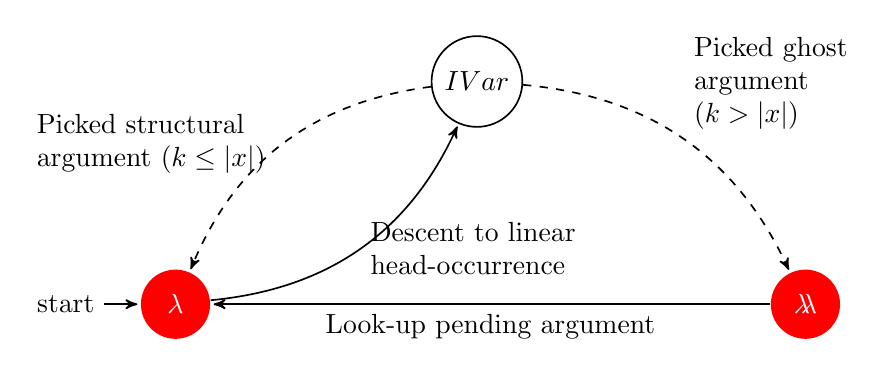
\begin{tikzpicture}[->,>=stealth',shorten >=1pt,auto,node distance=4cm,
    semithick]
\tikzstyle{every state}=[fill=red,draw=none,text=white]

\node[initial,state]
    (L) {$\lambda$};
\node[state,fill=white,draw=black,text=black]
    (V) [above right of=L, xshift=1cm] {$IVar$};
\node[state,node distance=8cm]
    (G) [right of=L] {$\ghostlmd$};

\path (L) edge [bend right]          node[right,text width=3cm]{Descent to linear head-occurrence} (V)
      (V) edge [bend right, dashed]  node[left,text width=3cm] {Picked structural argument ($k\leq|x|$)} (L)
          edge [bend left, dashed]   node[text width=2cm] {Picked ghost argument ($k>|x|$)} (G)
      (G) edge                       node {Look-up pending argument} (L)
;
\end{tikzpicture}
\caption{State machine underpinning the \emph{qnf} strand decomposition.}
\label{fig:qnf_strand_decomposition_statemachine}
\end{figure}



\begin{proposition}
\label{prop:qnf_traversals_are_finite}
Let $t \in \travsetnorm(M)$ for some \emph{quasi normal} term $M$. We have:
\begin{enumerate}[label=(\alph*)]
\item $lloc_M(\alpha) = \bot$ for all external lambda node $\alpha \in \NodesLmd$ occurring in $t$.
\item $t$ does not contain any internal variable node (\ie, all the internal nodes are $@$ nodes);
\item $t$ is finite.
\end{enumerate}
\end{proposition}
\begin{proof}
(a) and (b) are direct consequences of Proposition~\ref{prop:qnf_strand_decomposition}.
(c) Let's consider the cases of the strand decomposition of Proposition~\ref{prop:qnf_strand_decomposition}
observe that for the two transitions $\rightarrow S$ and $S \rightarrow S$, because $u_1$ and $u_2$ are spinal descents, the last node in the `next' strand ($x_1$ or $x_2$) must be a descendant (in the computation tree representation of $M$) of the first node from the `previous' strand ($\lambda\overline{\eta_1}$).
For transition $S\rightarrow G$, since both $u_1$ and $u_2$ are spinal descents, there are also paths in the tree, therefore since $\lambda\overline{y_2}$ points to $u_1$ we also have that $x_2$ is a descendant of $\lambda\overline{\eta_1}$. For transitions
$G \rightarrow S$ and $G \rightarrow G$, since $u_1$ and $u_2$ are spinal descents, $x_2$ is a descendant of $\lambda\overline{y_2}$, itself a descendant of $\lambda\overline{y_1}$.

Suppose $t$ is infinite then from the above strand decomposition we can construct an infinite path in the tree of $M$ which contradicts the fact that $M$ is a finitary term.
\end{proof}


%For any variable occurrence $x$ involved in a generalized redex $(\lambda x, A)$ for some subterm $A$, we will write $arg(x)$ to denote the root node of the $A$ in the term tree.
%For any node $m\in\NodesApp$ and index $i\geq0$ we will write $Child(m,i)$ to denote the $i$th child of $m$.
\begin{lemma}[Generalized redex argument lookup]
\label{lemma:genredex_lookup}
Let $x$ be a variable occurrence involved in a generalized redex in $gr(M)$.
\begin{enumerate}[label=(\roman*)]
    \item The path from the parent node of the redex argument down to $x$'s binder is of the form:
$$ @_r \cdot \lambda\overline{x_r} \cdots
@_2 \cdot \lambda\overline{x_2} \cdot @_1 \cdot \lambda\overline{x}$$
for $r\geq0$, where $@_r$ denotes the parent node of the redex argument, and $\lambda\overline{x}$ denotes $x$'s binder, such that $\lambda x$ is the $i$th lambda in the bulk lambdas $\lambda\overline{x}$ for $i\geq0$.

\item The argument of $x$ is precisely given by the $i_k$th child of node $@_k$ where $k$ is the smallest index verifying $i_k<|@_k|$ where:
\begin{align*}
    i_1 &= i \\
    i_{j+1} &= i_j - |@_j| + |\lambda\overline{x_{j+1}}| \qquad j\geq 0 .
\end{align*}
\end{enumerate}
\end{lemma}
\begin{proof}
(i) By definition of generalized redexes and lambda lists (Def.~\ref{dfn:generalized_redex}), $@_r$ necessarily occurs in the path from $\lambda\overline{x}$ to the root. Further the path from $@_r$ to $\lambda\overline{x}$ is necessarily a spinal descent (\ie, it contains only lambda and application nodes, and no variable node). Indeed, if it contained a variable node $z$ then the lambda-list at the subterm rooted at $z$ would be empty, in which case no argument could possibly form a generalized redex with $\lambda x$.

(ii) We show by induction on $k$ that $x$ is the variable abstracted by the $i_k$th lambda in $\lambda_l(\lambda\overline{x_k})$, which implies the result since by definition $\lambda x$ forms a generalized redex with the $i_k$th argument of $@_k$.
Base case $k=1$. By assumption, $\lambda x$ is the $i$th lambda in the bulk lambda $\lambda\overline{x}$. Let $k\geq 1$. By the induction hypothesis $\lambda x$ is the $i_{k-1}$ lambda in $\lambda_l(\lambda\overline{x_{k-1}})$.
substitution involved iBy definition of $k$ we have $i_{k-1}\geq|@_{k-1}|$, therefore by definition of $\lambda_l$, the long-application $@_{k-1}$ has the effect of popping exactly $|@_{k-1}|$ arguments from the lambda-list, and the following abstraction $\lambda\overline{x_k}$ then adds $|\lambda\overline{x_k}|$ more lambdas in front of the lambda list. Hence $\lambda x$ gets moved to position $i_{k-1} - |@_{k-1}| + |\lambda\overline{x_k}| = i_k$ in the lambda list at $\lambda\overline{x_k}$.
\end{proof}

\paragraph{Traversal bisimulation}

For any term $M$ we define $\travset^\dagger(M)$ as the subset of traversals of $\travsetnorm(M)$ ending
with either a structural node or an external ghost variable (\ie, not ending with an internal ghost variable nor a ghost lambda).
Observe that every traversal in $\travsetnorm$ has a traversal extension in $\travset^\dagger$.
Indeed, if $t \in \travsetnorm$ ends with an internal ghost variable or a ghost lambda then repeatedly applying
rules \rulenamet{Var} and \rulenamet{Lmd} yields a traversal ending with an external node.

\begin{definition}[Traversal bisimulation]
\label{def:bisimilar_terms}
Let $M$ and $N$ be two terms. Let $\phi\colon \justseqset(N) \rightarrow\justseqset(M)$ be a function from the justified sequences of $N$ to justified sequences of $M$. We define the state transition system $(X, R_\phi, \rightarrow)$ as:
\begin{itemize}
    \item \emph{States}: $X$ is the disjoint union $\travset^\dagger(M) + \travset^\dagger(N)$.

    \item \emph{Binary relation $R_\phi\subseteq X \times X$} defined for any traversals $t, u \in X$ as:
    $$ t~R_\phi~u  \ \iff \ \begin{cases}
        t\in\travset^\dagger(M)\\
         u\in\travset^\dagger(N) \\
         \phi(u) = t
    \end{cases}
    $$

    \item \emph{Transitions} For any traversals $t, t' \in \travset^\dagger(M)$ we write $t \rightarrow_M t'$ just if $t'$ is a minimal extension of $t$ that remains in $\travset^\dagger(M)$. (\ie, $t'$ extends $t$ using rules of Table~\ref{tab:normalizing_trav_rules} and any occurrence strictly between the last occurrence in $t$ and $t'$ is an either internal ghost variable or a ghost lambda node. We define relation $\rightarrow_N$  identically, and write $t \rightarrow_X t'$ if either $t \rightarrow_M t'$ or $t \rightarrow_N t'$ holds for $t, t' \in X$.
\end{itemize}

The two terms $M$ and $N$ are \defname{$\phi$-bisimilar} just if the relation $R_\phi$ defines a bisimulation over $X$ with respect to $\rightarrow_X$:
\begin{itemize}
    \item (B1) for all $t_1, t_2 \in \travset^\dagger(M), u_1 \in \travset^\dagger(N)$ with $t_1~R_\phi~u_1$ and $t_1 \rightarrow_M t_2$ there is $u_2 \in \travset^\dagger(N)$ such that $u_1 \rightarrow_N u_2$ and $t_2~R_\phi~u_2$.
    \item (B2) for all $t_1 \in \travset^\dagger(M), u_1, u_2 \in \travset^\dagger(N)$ with $t_1~R_\phi~u_1$ and $u_1 \rightarrow_N u_2$ there is $t_2 \in \travset^\dagger(M)$ such that $t_1 \rightarrow_M t_2$ and $t_2~R_\phi~u_2$.
\end{itemize}
\end{definition}

\begin{lemma}
\label{lem:bisimulation_isomorphism}
If $M$ and $N$ are $\phi$-bisimilar and
(i) the restriction of $\phi$ to $\coresymbol(\travset^\dagger(N))$ is injective;
(ii) there exists a variable name mapping $\rho: \VarSet^*(N) \rightarrow \VarSet^*(M)$ such that for any variable names $\alpha\in\VarSet^*(N)$, the functions $\phi$ and $\coresymbol_\alpha$ commute modulo $\rho$:
$$ \coresymbol_{\rho(\alpha)}(\phi(u)) = \phi(\coresymbol_{\alpha}(u))$$
then $\coresymbol(\travset(N)) \cong \coresymbol(\travset(M))$.
\end{lemma}
\begin{proof}
Let us consider $\phi$ as a function from $\coresymbol(\travset^\dagger(N))$ to $\coresymbol(\travset^\dagger(M))$.
It is \emph{well-defined}: $\travset^\dagger(N)$ is by definition the transitive closure of the empty traversal by $\rightarrow_N$, so for any traversal $u$ of $\travset^\dagger(N)$, repeatedly applying (B2) for each step of its $\rightarrow_N$ derivation shows that $t = \phi(u) \in \travset^\dagger(M)$. By commutativity of $\coresymbol$ and $\phi$ this yields $\coresymbol(t)=\phi(\coresymbol(u)) \in \coresymbol(\travset^\dagger(M))$.
Similarly, it is \emph{surjective} by (B1) because $\travset^\dagger(M)$ is the transitive closure of the empty traversal by $\rightarrow_M$. Finally it is \emph{injective} by assumption.
Hence we have $\coresymbol(\travset^\dagger(N)) \cong \coresymbol(\travset^\dagger(M))$, and because $\coresymbol$ eliminates internal nodes from traversals, we also have $\coresymbol(\travset(N)) \cong \coresymbol(\travset(M))$.
\end{proof}

%%%%% Soundness of leftmost liner reduction
We now show that normalizing traversals implement substitution in the sense that
the sets of traversals $\travsetnorm$ before and after reduction are identical up to some mapping between nodes of the term and its reduct.
\begin{proposition}[Traversals are sound for linear reduction]
\label{prop:ulctrav_impl_linear_reduction}
Let $M$ be an untyped term.
$$M \rightarrow_l N \implies \coresymbol(\travsetnorm(M)) \cong \coresymbol(\travsetnorm(N)) \ .
$$
\end{proposition}
%\begin{proof}
\proofatend
Suppose that $M \rightarrow_l N$. Let $x$ denote the leftmost linear variable occurrence in $M$ and
let $(\lambda x, A)$ be the generalized redex involving it, so that $N$ is the term obtained after
firing the generalized redex $(\lambda x, A)$. A property of linear head reduction is that the reduct contains the original
term itself, modulo alpha conversion and relabelling of the \emph{lloc} node. This induces an implicit map $\Phi$ from nodes
of the reduct $N$ to those of $M$:
$$\Phi : \ExtendedNodes(N)  \rightarrow \ExtendedNodes(M) $$
which maps nodes from the substituted subterm in $N$ to the corresponding nodes under argument $A$ in $M$;
and every node in $N$ that is not involved in the substitution, to its counterpart in $M$.

The substitution involved in the leftmost linear reduction affects the computation tree in three possible ways depending on the structure and number of $x$'s operands:
\begin{description}[itemindent=1em]
    \item[Case 1] $x$ has at least one operand ($|x|>0$) and $A$ is an abstraction;
    \item[Case 2] $x$ has at least one operand ($|x|>0$) and $A$ is not an abstraction;
    \item[Case 3] $x$ is unapplied ($|x|=0$).
\end{description}

%%%%%%%%%%% Summary of the proof %%%%%%
% Observe first that the nodes of the subterm $A$$ map 1-1 to the nodes of
% the subterm $\phi(x)$ in $N$.
% We can therefore defined $\psi$ such that all the nodes in $t$ hereditarily justified by the root of $A$ are
% mapped by $\psi$ to the corresponding nodes in $N$. We omit the full details of the induction which is purely
% mechanical and straightforward. The idea being that $N$ is obtained by transposing the structure of the subterm
% $A$ in place of $x$ with the additional relabelling of $x$'s parent $\lambda\overline{y}$ as
%$\lambda\overline{y}\overline{z}$ where $\lambda\overline{a}$ denotes the root of $A$. The key observation
% is that this relabelling is innocuous in the sense that all rules applied to $t$ in $M$ can also be
% applied to $\psi(t)$ in $N$.
%
% It is trivial to see show traversal of $M$ can be bisimulated in $N$ all the way to variable $x$.
% It's more delicate to show that further extensions can also be bisimulated, in particular traversals of
%  the subterm $R$ in $M$ can be bisimulated by traversals of $R'$ in the reduct $N$.
% We omit the tedious details here for succinctness.  The key observation is that
% because the enabling relation $\enables$ in $R$ is preserved through $\phi$ after substitution and
%  alpha-conversion in the subterm $R'$, the subsequent traversal
%  of argument $R$ in $M$ can be bisimulated by traversing $R'$ in
%   the reduct $N$ using the exact same traversal rules used to traverse $M$.
%%%%%%%%%%%%%%%%%%

We proceed by showing that for each of the three cases, there is an injection $\phi$ such that $M$ and $N$ are $\phi$-bisimilar.

\begin{description}[itemindent=0em,leftmargin=0cm]
    \item[Case 1]
    The reduction is represented on Figure~\ref{fig:firing_genredex_effect_on_tree_with_operands_and_lambda_argument}
    where $x$ has some operand ($|x|>0$), and $A$ is an abstraction $\lambda\overline{y}. R$.

    Let $\lambda\overline{x}$ denote $x$'s binding lambda node in $M$, $i$ denote $x$'s binding index, and $@_a$ denote the parent node of the subterm $A$.

    After reduction:
    (i) Node $x$ gets replaced by an application node $@_x$ and its existing children are preserved.
    (ii) The subterm $\lambda\overline{y}'. R'$, obtained from $R$ by renaming variable afresh to avoid variable capture, becomes the operator child of $@_x$.  (Note that we write $\lambda\overline{y}'$ to distinguish the root node of $R'$ from the root $\lambda\overline{y}$ of $R$ in $N$, even though the bound variable names are $\overline{y}$ for both nodes.)

    We thus have $\Phi(@_x) = x$, $\Phi(\lambda\overline{y}') = \lambda\overline{y}$, and $\Phi$ maps each node from subterm $\lambda\overline{y}'. R'$  to the corresponding node under $\lambda\overline{y}.R$.

%%%%%%%%% Figure showing the substitution Case 1.
\begin{figure}[htbp]
    \centering
    \begin{tikzpicture}[baseline=(root.base),level distance=5ex,inner ysep=0.5mm,sibling distance=8mm]
    \node (root){}
            child[dashed]{node{$@_{a}$}
                child[solid]{node{$\lambda\overline{\xi}_a$}
                    child[dashed]{node{$@$}
                        child{node{$\lambda\ldots$}
                            child[solid]{node{$@$}
                                child[solid]{node{$\lambda\overline{z}$}
                                    child[solid,level distance=5ex]{node {$x$}
                                        child{node{$B_1$}}
                                        child{node{$\ldots$}}
                                        child{node{$B_q$}}
                                        }
                                    edge from parent node[above left]{$0$}
                                }
                                child[dashed]{node{}}
                            }
                        }
                        child[dashed]{node{}}
                    }
                    edge from parent node[above left]{$0$}
                }
                child[dashed]{node{\ldots}}
                child[solid]{node{$\lambda\overline{y}$}
                    child{node{$R$}}
                }
                child[dashed]{node{\ldots}}
            }
    ;
    \node (root2) at (8,0) {}
        child[dashed]{node{$@_{a}$}
            child[solid]{node{$\lambda\overline{\xi}_a$}
                child[dashed]{node{$@$}
                    child{node{$\lambda\ldots$}
                        child[solid]{node{$@$}
                            child[solid]{node{$\lambda\overline{z}$}
                                child[solid,level distance=5ex]{node {$@_x$}
                                    child{node{$\lambda\overline{y}'$}
                                        child{node{$R'$}}
                                    }
                                    child{node{$B_1$}}
                                    child{node{$\ldots$}}
                                    child{node{$B_q$}}
                                    }
                                edge from parent node[above left]{$0$}
                            }
                            child[dashed]{node{}}
                        }
                    }
                    child[dashed]{node{}}
                }
                edge from parent node[above left]{$0$}
            }
            child[dashed]{node{\ldots}}
            child[solid]{node{$\lambda\overline{y}$}
                child{node{$R$}}
            }
            child[dashed]{node{\ldots}}
        }
    ;
    \draw[<-] ([xshift=2.5cm,yshift=-2cm]root.east) -- +(2cm,0)
    node[midway, above] {$\Phi$};
    \end{tikzpicture}
    \caption{(Case 1) Reduction $M\rightarrow_l N$ where node $x$ has at least one operand, and $A$ is a non-dummy
     abstraction $\lambda\overline{y} . R$. Linearly firing  generalized redex $(\lambda x, A)$ for $x$ in $M$ (left)
     yields $N$ (right) where $R'$ is a copy of $R$ with fresh names to avoid variable capture.
    Function $\Phi$ maps nodes from the right tree to the left tree.}
    \label{fig:firing_genredex_effect_on_tree_with_operands_and_lambda_argument}
    \end{figure}


Observe that $\Phi$ has the following properties:
\begin{enumerate}[label=(\roman*)]
    \item $\Phi$ preserves the parent-child relation for lambda and variable nodes: for any lambda or variable node $n$, the child nodes of $n$'s image by $\Phi$ are the image of the $n$'s children. (This is not true for application node $@_x$, however);

    \item $\Phi$ is naming-consistent: any two variable nodes sharing the same name  in $N$ map to variable nodes with same name in $M$;

    \item $\Phi$ preserves variable binding: it maps the binder lambda node of a variable node $z$ in $N$ to the binder in $M$ of $\Phi(z)$;

    \item hence $\Phi$ preserves the enabling relation: if $n_1 \enables_i n_2$ in $N$ for $i\geq 0$, $n_1,n_2 \in \Nodes(N)$ then $\Phi(n_1) \enables_i \Phi(n_1)$ as long as $(n_1,n_2) \neq (@_x,\lambda\overline{y}')$.

    \item $\Phi$ preserves node types: images of external and internal nodes are respectively external and internal nodes; images of variable/@-nodes are variable/@-nodes; images of lambda nodes are lambda nodes; images of ghost and structural nodes are respectively ghost and structural;

    \item $\Phi$ preserves node arity. In particular $|x| = |@_x|$ since $@_x$'s operator does not contribute to its arity;

    \item $\Phi$ is not injective: since for any node in $R'$ there is a corresponding node in $R$ that is mapped to the same node in $M$.
\end{enumerate}

Let $\justseqset^P$ denote the subset $\justseqset$
consisting of justified sequences verifying the P-view-path correspondence:
the P-view at every occurrence of an internal node is precisely the path from the root to that node in the computation tree. By Property~\ref{prop:tree_path_charact} we have $\travset \subseteq \justseqset^P$.

We define $\phi$ as an extension of $\Phi$ to justified sequences of $\justseqset^P$ of $N$ as follows:
(i) maps all other occurrences to their image by $\Phi$;
(ii) it preserves all justification pointers except for $@_x$ and $\lambda\overline{y}'$;
(iii) inserts in-between each occurrence of $x$ and its immediately following lambda-node, the corresponding \emph{argument lookup} of $x$. Formally $\phi = \phi_1 \circ \phi_2$ where
\begin{align*}
\phi_1 \colon & \justseqset^P(N) \rightarrow \justseqset(M) \\
& \epsilon \mapsto \epsilon  \\
& t \cdot n \mapsto \phi(t) \ \cdot \Phi(n) &\mbox{$\Phi(n)$ has same link label and length as $n$, for $n\not\in \{ @_x, \lambda\overline{y} \}$}\\
 & t \cdot @_x \mapsto \phi(t) \ \cdot x &\mbox{$x$ points to the first occurrence of $x$'s binder in $\pview{t}$} \\
& t \cdot \lambda\overline{y}' \rightarrow \phi(t) \ \cdot \lambda\overline{y} &\mbox{$\lambda\overline{y}$ points to the last occurrence of $@_a$ in $\pview{t}$.}
\end{align*}
and $\phi_2$ is the function that inserts the argument lookup sequence of ghost nodes between each occurrence of $x$ and $\lambda\overline{y}$ in a justified sequence. Observe that the argument lookup of $x$ is entirely statically determined and thus can be reconstructed from any (visible) traversal $t_{\leq x}$ of $M$ by repeatedly instantiating rules \rulenamet{Lmd} and \rulenamet{Var} starting from $t_{\leq x}$ until reaching node $\lambda\overline{y}$.

The following example illustrates how $\phi$ is calculated on a generic
traversal $u$ of $N$ involving the lloc variable $x$:
\begin{eqnarray*}
    u &=& \Pstr[10pt]{ \ldots (aa){@_a} \cdot (la){\bulklambda{\xi_a}} \cdot \ldots (a1){@_1} \cdot (l1){\bulklambda{\xi_1}} \cdot @ \ldots \bulklambda{z} \cdot (ax){@_x} \cdot (ly-ax,20:0){\bulklambda{y}'} }
    \\
    \phi_1(u) &=& \Pstr[10pt]{ \ldots (aa){@_a} \cdot (la){\bulklambda{\xi_a}} \cdot \ldots (a1){@_1} \cdot (l1){\bulklambda{\xi_1}} \cdot @ \ldots \bulklambda{z} \cdot (x-l1,30:i) x \cdot (ly-a,25){\bulklambda{y}} }
    \\
    \phi(u) = \phi_2(\phi_1(u)) &=& \Pstr[10pt]{ \ldots (aa){@_a} \cdot (la){\bulklambda{\xi_a}} \cdot \ldots (a1){@_1} \cdot (l1){\bulklambda{\xi_1}} \cdot @ \ldots \bulklambda{z} \cdot (x-l1,30:i) x \cdot \ghostlmd \cdot \ghostvar \ldots \ghostlmd \cdot \ghostvar \cdot (ly-a,20:i_a){\bulklambda{y}} }
\end{eqnarray*}

Some immediate properties:
\begin{itemize}
\item $\phi_1$, and $\phi$ are well defined since by the P-view-path property, $x$'s binder and (resp.~$@_a$) must necessarily occurs in the P-view at $x$ (resp.~$\lambda\overline{y}'$).

\item The restriction of $\phi$ to $\coresymbol(\travset^\dagger(N))$
coincides precisely with the element-wise structure-preserving\footnote{Recall that two justified sequences over two distinct terms share the same structure just if their constituting nodes are of the same kind (variable/@ nodes or lambda node), have the same link labels, and same pointer lengths.} extension of $\Phi$ over justified sequences.
This is because $\phi_1$ only alters justification pointers of internal nodes ($@_x$ and $\lambda\overline y$) and $\phi_2$ only inserts internal nodes, while justified sequences in $\coresymbol(\travset^\dagger(N))$ do not contain any external node.

\item The restriction of $\phi$ to $\coresymbol(\travset^\dagger(N))$, is injective.
%%%%%%% Short summary: because when a traversal extends in more than one possible way (with rule \rulenamet{IVar}), then either the next possible occurrences all have distinct justification pointers, or $\Phi$ maps them to distinct nodes in $M$.
Suppose that $\coresymbol(u)\neq\coresymbol(v)$ for $u,v\in\travset^\dagger(N)$ then we must have $u\neq v$.
Let $s$ denote the longest common prefix of $u$ and $v$; and $n_1, n_2$ the nodes immediately following $s$ in $u$ and $v$
respectively. We have $s \rightarrow_N s \cdot n_1$ and $s \rightarrow_N s\cdot n_2$ with $n_1\ne n_2$ therefore $n_1, n_2$ are necessarily traversed
by the non-deterministic rule \rulenamet{IVar}. Hence they must both be external nodes and therefore they are not eliminated after applying $\coresymbol$: the last occurrence of $\coresymbol(s\cdot n_1)$ and $\coresymbol(s\cdot n_2)$ are different. Since $\Phi$ maps distinct external sibling nodes in $N$ to distinct sibling nodes in $M$, we necessarily have
$\phi(\coresymbol(s\cdot n_1))\neq \phi(\coresymbol(s\cdot n_2))$.
%%%%%%%%%

\item $\coresymbol$ and $\phi$ commute modulo the implicit renaming function $\rho: \VarSet^*(N) \rightarrow \VarSet^*(M)$ underlying $\Phi$. Formally, for any variable names $\alpha\in\VarSet^*$ occurring in $N$ we have:
$$
\phi(\coresymbol_\alpha(u)) = \coresymbol_{\rho(\alpha)}(\phi(u)) \ .
$$
This is shown by an easy induction and by assuming, without loss of generality, that variable names are not reused in either $M$ or $N$: each variable name is introduced by at most one lambda node in each term. (This condition can always be met via alpha-conversion.)
\end{itemize}

We now show that $M$ and $N$ are in $\phi$-bisimulation by induction on the traversals rules.

\emph{Base case}: $\rulename{Root}_\normalizing$ The empty traversal in $M$ is trivially the image by $\phi$ of the empty traversal in $N$. Same for the two singleton traversals consisting of the root nodes of $M$ and $N$.

\emph{Induction}: Let $u\in \travset^\dagger(N)$, $t\in\travset^\dagger(M)$ with $t = \phi (u)$ and $m, n$ denote respectively the last node in $t$ and $u$. We prove both directions by case analysis on the \emph{first} traversal rule used to extend $t$ (resp.~$u$).

Observe that the result holds trivially up until the traversal in $M$ reaches occurrence $x$ since one can use the exact same rules used to traverse $M$ in order to traverse the corresponding node in $N$, and reciprocally for traversals of $N$ until reaching node $@_x$. The crucial part of the induction takes place when traversing the \emph{lloc} variable $x$ (or $@_x$ in $N$).

\begin{itemize}[itemindent=0.5em, leftmargin=0.5em]
    \item $\rulename{App}_\normalizing$ We have $m = \Phi(n)$.

    (B1) Suppose $t$ extends to $t'$ with the application rule then $m, n \in\NodesApp$. Then the last occurrence $m'$ in $t'$ is the unique node verifying $m \enables_0 m'$.  Since $\Phi$ does not map $@_x$ to an application node we necessarily have  $n \neq @_x$. Thus $\phi$ preserves the enabling relation at $n$, and we can use the application rule in $N$ to extend $u$ into $u' = u \cdot n'$ where $n \enables_0 n'$ and $\phi(n') = m'$.

    (B2) Suppose $u'$ extends traversal $u$ with the application rule then the last occurrence $n$ in $u$ is an application node.
    If $n\neq@_x$ then $\phi$ preserves the enabling relation at $n$ and therefore the application rule can be used in $M$ to simulate $u'$.

    %%%%%%%%%%%%%%%%% Case t ends with lloc variable occurrence x
    Otherwise, $n=@_x$ and since $t = \phi(u)$ we must have $m = \Phi(@_x) = x$.
    and $u' = u \cdot \lambda\overline{y}'$.
    Let $@_j$ and $\lambda\overline{\xi_j}$ for $1\leq j\leq a$, $a\geq 1$ denote respectively the application and lambda nodes in the spinal descent
    from $@_a$ to $x$'s binder. So that $\lambda\overline{\xi_1}$ is $x$'s binder, $@_1$ its parent,  and $@_a$ is $\lambda\overline{y}$'s parent.
    By Lemma~\ref{lemma:genredex_lookup}, $@_a$ is precisely the lowest application node in the spinal descent
    from $@_a$ to $\lambda\overline{\xi_1}$ verifying $|@_a| >  i_a$,
        where $i_a = i + \sum_{1\leq j< a} (|\lambda\overline{\xi_j}| - |@_j|)$.
    This formula precisely captures the ``pending argument lookup'' algorithm implicitly
    implemented by the rules \rulenamet{Lmd} and \rulenamet{Var}:
    with exactly $i_a$ instantiations of those two rules, traversal $t$ gets extended by $2(i_a-1)$ ghost nodes followed
    by the root of $A$:
            $$ t \rightarrow_M t \cdot v \cdot \lambda\overline{y}$$
    where  $v$ is a \emph{pending argument lookup}.
    Therefore by definition of $\phi$ if $v$ denote the argument lookup of $x$ we have:
    $\phi(u')
    = \phi(u \cdot \lambda\overline{y}')
    = \phi(u) \cdot \phi(\lambda\overline{y}')
    = t \cdot v \cdot \lambda\overline{y} \in \travset^\dagger(M)$.
    %%%%%%%%%%%%%%%%%%

    \item $\rulename{Lam}^@_\normalizing$
    (B1) follows from the fact that parent-child relation is preserved by $\Phi$
    (B2) Suppose $n \neq \lambda\overline{z}$ then it follows again from the fact that parent-child relation is preserved by $\Phi$.
    Otherwise, we have $n = \lambda\overline{z}$ and $u \rightarrow_N u \cdot \lambda\overline{y}'$ can be simulated in $M$ using rule $\rulename{Lam}^{\sf var}$: $t \rightarrow_M t \cdot x$.

    \item $\rulename{Lam}^{\sf var}_\normalizing$
    We have already shown that  $\phi$ preserves the local child-parent relationship for lambda nodes; node types, and arity of lambda nodes.
    It remains to show that any $\enables$-enabler of $m$ that is visible at  $u$ is mapped to an enabler of $n$ that is visible in $\phi(u)$.

    Since the last node of $t$ and $u$ are structural lambda nodes, their P-view do not contain any ghost node nodes, and in particular the argument lookups inserted by $\phi_2$ are not involved in the P-view calculation. Hence $\pview{\phi(u)} = \pview{\phi_1(u)}$.
    But by the P-view path characterization of traversals $\pview{\phi_1(u)}$ is precisely the path in $M$ from $\Phi(n)$ to the root of $M$,
    and $\pview{u}$ is the path in $N$ from $n$ to the root of $N$.

    If $n$ is not under $\lambda\overline{y}'.R'$ then the path to the root is not impacted by the reduction and therefore the path in $M$ and $N$ are identical modulo $\phi$: we thus have $\pview{\phi_1(u)} = \phi_1(\pview{u})$.
    Otherwise if $n$ is under $\lambda\overline{y}'.R'$ then the path from $m$ to the root in $M$ is precisely the element-wise image by $\Phi$ of the path from $n$ to the root in $N$ with the exclusion of the spinal descent from $@_a$ to $@_x$. But by construction of $N$, none of the variable in $R'$ are bound by the lambda nodes in the spinal descent.

    Hence we the rule $\rulename{Lam}^{\sf var}_\normalizing$ used to extend  $u$ can also be used to extend $t$, and reciprocally.

    \item $\rulename{Lam^\ghostlmd_\normalizing}$
    This case is excluded since $t$ and $u$ belong to $\travset^\dagger(M)$ and
    $\travset^\dagger(N)$ respectively and therefore their last occurrence cannot be a ghost lambda.

    \item $\rulename{Var_\normalizing}$
    (B2) Since $\Phi$ maps external variable nodes to external variable nodes,preserves the parent-child relation for variable nodes and $\phi$ preserves the justification pointer of external variable nodes, if this rule can extend traversal $u$ with node $n'$ then the same rule can be used to extend $t$ with $\phi(n')$.

    (B1) Suppose that $t$ ends with \emph{lloc} variable $x$ in which case $t' = t \cdot \lambda\overline{y}$, then
        we can just take $u = u' \cdot @_x$ and conclude exactly like we did for case $\rulename{App}_\normalizing$ (B2).
    Otherwise, if $m\neq x$, we conclude like in case (B1).

    \item $\rulename{IVar_\normalizing}$ $\Phi$ preserves node types, arity of variable nodes. It remains to show that it preserves \emph{arity threshold} of traversals: In an argument lookup, all occurrences are ghost with arity $0$ therefore they do not affect the arity threshold calculation. Hence $\arth(\phi(u))=\arth(\phi_1(u))$. Further $\Phi$ preserves arity and maps external and internal nodes to external and internal nodes respectively, thus $\arth(\phi_1(u))=\phi_1(\arth(u))$.
    Hence the rule $\rulename{Var_\normalizing}$ used to extend $u$ can be used to extend $t$, and reciprocally.

\end{itemize}

%%%%%%%% CASE 2
\item[Case 2] where $x$ has at least one operand ($|x|>0$) and $A$ is an application ($|\overline{y}|=0$). The root lambda node of $A$ is therefore a dummy lambda: $A = \lambda. R$. Let $r$ denote the root node of $R$, which is either a variable if $R$ is in head-normal form, or an $@$-node otherwise.
The tree of the reduct $N$ is obtained from $\ctree(M)$
by substituting $x$'s label with that of $r$ (modulo variable renaming to avoid capture if $r$ is a variable node) and prepending $r$'s children to existing $x$'s children. Other nodes, including $x$'s parent lambda node, remain untouched. Let $r'$ denote this updated node in the reduct $N$.
This transformation yields an implicit mapping function $\Phi : \ExtendedNodes(N)\rightarrow \ExtendedNodes(N)$ such that $\Phi(r') = x$.
Although $\Phi$ does not preserve the arity of $x$, it does not affect the arity threshold of traversals since $|r'| = |x| + |r|$.
We can then extend $\Phi$ to a function $\phi$ on justified sequence and show by induction that it yields a bisimulation similarly to the previous case.

%%%%%%% CASE 3
\item[Case 3] where $x$ is unapplied ($|x|=0$).
After reduction, node $x$ gets replaced by subterm $A$ and the label of $x$'s parent lambda node gets concatenated with the label of $A$'s root node:
the parent lambda node $\lambda\overline{z}$ of $x$ in $M$ becomes $\lambda\overline{z}\overline{y}'$ in the reduct $N$.
Like in the first case, we can define a function $\phi$ such that
 traversals of $M$ of the form $\ldots \lambda\overline{z}\cdot x \cdot v \cdot \lambda\overline{y} \cdot \ldots$, where $v$ is an argument lookup, are images of traversals in $N$ of the form $\ldots \cdot \lambda\overline{z}\overline{y}' \ldots$. Once again, although the arity of $x$ is not preserved, this does not affect the arity threshold because $|\lambda{\overline{z} \overline{y}'}| =
 |\lambda{\overline{z}}| +  |\lambda{\overline{y}}|$.
\end{description}

%%%%%%%%%%%%%%%%% End of case where t ends with lloc variable occurrence x

Hence $M$ and $N$ are in $\phi$-bisimulation, thus because $\phi$ is injective and commutes with $\coresymbol$, by Lemma~\ref{lem:bisimulation_isomorphism} the two sets of traversals are isomorphic.
\endproofatend
%\end{proof}


\begin{proposition}[Traversals are sound for trivial reduction]
\label{prop:ulctrav_sound_for_trivialreduction}
    Let $M$ be an untyped term containing only trivial redexes, and $N$ the reduct obtained by firing the leftmost innermost trivial redex, then $\coresymbol(\travsetnorm(M)) \cong \coresymbol(\travsetnorm(N))$.
\end{proposition}
\proofatend
%\begin{proof}
Let's consider the tree structure at the trivial redex on Figure~\ref{fig:reducing_trivialredex}. It is of the form $(\lambda \overline{x} . T) A_1 \ldots A_r$ for $r\geq1$ where $(x_1, A_1)$ forms the leftmost trivial redex.
    Two cases must be considered:

    \begin{figure}[htbp]
        \centering
        \begin{tikzpicture}[baseline=(root.base),level distance=5ex,inner ysep=0.5mm,sibling distance=13mm]
        \node (root_rGt1_M){}
                child[dashed]{node{$\lambda\overline\eta$}
                    child[solid]{node{$@$}
                        child[solid]{
                            node{$\lambda x_1 x_2 \ldots x_n$}
                            child[solid,level distance=5ex]
                                {node {$T$}}
                            edge from parent node[above left]{$0$}
                        }
                        child{node{$A_1$}}
                        child[dashed]{node{$\ldots$}}
                        child{node{$A_r$}}
                    }
                };
        \node (root_rGt1_N) at (7,0) {}
                child[dashed]{node{$\lambda\overline\eta$}
                    child[solid]{node{$@$}
                        child[solid]{
                            node{$\lambda x_2 \ldots x_n$}
                            child[solid,level distance=5ex]
                                {node {$N$}}
                            edge from parent node[above left]{$0$}
                        }
                        child{node{$A_2$}}
                        child[dashed]{node{$\ldots$}}
                        child{node{$A_r$}}
                    }
                };
        \node (root_rEq1_M) at (0,-3) {}
                child[dashed]{node{$\lambda\overline\eta$}
                    child[solid]{node{$@$}
                        child[solid]{
                            node{$\lambda x_1 x_2 \ldots x_n$}
                            child[solid,level distance=5ex]
                                {node {$T$}}
                            edge from parent node[above left]{$0$}
                        }
                        child{node{$A_1$}}
                    }
                };
        \node (root_rEq1_N) at (7,-4) {}
                child[dashed]{node{$\lambda\overline\eta~x_2 \ldots x_n$}
                    child[solid]{node{$N$}
                    }
                }
        ;
        \draw[->] ([xshift=1.5cm,yshift=-1cm]root_rGt1_M.east) -- +(3.5cm,0)
        node[midway, above] {trivial reduction};
        \draw[->] ([xshift=1.5cm,yshift=-1.5cm]root_rEq1_M.east) -- +(3.5cm,0)
            node[midway, above] {trivial reduction} ;
        \end{tikzpicture}

        \caption{Reducing a (leftmost innermost) trivial redex. Case $r>1$ (top) and $r=1$ (bottom).}
\label{fig:reducing_trivialredex}
    \end{figure}

    \begin{description}
    \item[Case $r>1$] Because the structure of the tree is preserved after reduction, there is an implicit injection $\Phi$ from nodes of the reduct $N$ to nodes of $M$. Let $\phi$ denote its element-wise structure-reserving  extension to justified sequences.

    Firstly, $M$ and $N$ are in $\phi$-bisimulation. We omit the details, the key observations are:
    (i) Since $x_1$ does not occur in $T$, the term $A_1$ will never be traversed in $N$.
    (ii) Only nodes hereditarily justified by $\lambda x_1 \ldots x_n$ see their label (or link label) changed after applying $\Phi$. But since those are external nodes, they get filtered out by the core projection $\coresymbol$.
    (iii) The arity of node $\lambda x_2 \ldots x_n$ increases by $1$ after applying $\Phi$, but it does not impact the arity threshold of traversals because the arity of the application node also increases by $1$.

    Secondly, since $\Phi$ is injective, so is its element-wise extension to justified sequences.

    Finally $\phi$ and $\coresymbol$ commute. This is shown by an easy induction, observing that nodes $@$ and $\lambda x_2\ldots x_n$ necessarily occur consecutively in a traversal of $N$, and because $|@| = |\Phi(@)| -1$ and $|\lambda x_2\ldots x_n| = |\Phi(\lambda x_2\ldots x_n)| - 1$, the core projection is preserved modulo $\Phi$.

    Hence by Lemma~\ref{lem:bisimulation_isomorphism} the two sets of traversals are isomorphic.

    \item[Case $r=1$] Depicted on Figure~\ref{fig:reducing_trivialredex} (bottom). The tree structure is altered: the application node and the argument $A_1$ are eliminated in the reduct. There is an implicit injection $\Phi$ from nodes of $N$ to nodes of $M$. We extent this function to \emph{occurrences} of nodes as follows. Let's introduce the abbreviation $\overline{y} = \overline\eta x_2 \ldots x_n$.
    \begin{align*}
        \Phi\colon O_4(N) &\rightarrow O_4(M) \\
        (n,p,d,k) &\longmapsto (\Phi(n),p,d,k) & \mbox{if $n\neq\lambda\overline{y}$} \\
        (\lambda\overline{y},p,d,k) &\longmapsto (\lambda\overline\eta,(x_2 \ldots x_n \cdot p),d,k)
    \end{align*}
    So in particular, $\Phi$ maps occurrences of $\lambda\overline{y}$ to occurrences of $\lambda\overline\eta$ with binding variables $x_2 \ldots x_n$ appended to $\overline\eta$.
    \begin{equation}
        \Phi(\lambda\overline{y})
        =
        \lambda\overline\eta^{[x_2\ldots x_n]}
        \label{eqn:phi_maps_lambday_to_lambdaeta}
    \end{equation}
    Observe also that $\Phi$ commutes with the rebinding operation: because in the case of $\lambda\overline{y}$, $\Phi$ appends variable names to the left whereas the rebinding operation appends variables names to the right.

    We extend $\Phi$ to justified sequences by taking the element-wise extension $\phi$ with the following additional modification: any occurrence of node $\lambda\overline{y}$ in a traversal of $N$ gets expanded by $\phi$ into the three occurrences $\lambda\overline\eta \cdot @ \cdot \lambda\overline{x}$ in $M$.

    We have the following properties:
    \begin{itemize}
    \item $\phi$ is injective. It follows from the fact that $\Phi$ is itself injective.

    \item $\phi$ and $\coresymbol$ commute. This is because $\phi$ carries over the list of pending lambdas and the core symbol operation adequately implements merging of nodes $\lambda\overline\eta$ and
    $\lambda\overline x_1 \ldots x_n$ into
    $\lambda\overline\eta x_2 \ldots x_n$. Formally:

    Let $u$ be a traversal of $\travset^\dagger(N)$
    ending with $\lambda\overline{y}$ that is
    $u = u_1 \cdot \lambda\overline{y} $ for some traversal $u_1$.
    The sequence $\phi(u)$ is of the form
    $\phi(u) = \phi(u_1) \cdot \lambda\overline{\eta} \cdot @ \cdot \lambda\overline{x}$. Let $\overline\alpha$ be the list of pending lambdas at $u_{\leq \lambda\overline{y}}$. There are two cases:

    Suppose $\lambda\overline\eta$ is internal. We have:
    \begin{align*}
        \coresymbol_{\overline\alpha}(\phi(u))
        &=  \coresymbol_{\overline\alpha}(\phi(u_1) \cdot \lambda\overline{\eta} \cdot @ \cdot \lambda\overline{x})
            & \mbox{(def.~of $\phi(u)$)}
        \\
        &=  \coresymbol_{\overline{x}\overline\alpha}(\phi(u_1) \cdot
        \lambda\overline\eta \cdot @)
            & \mbox{(def.~of $\coresymbol$)}
        \\
        &=  \coresymbol_{pop_1(\overline{x}\overline\alpha)}(\phi(u_1) \cdot
        \lambda\overline{\eta})
            & \mbox{(def.~of $\coresymbol$ and $|@|=1$)}
        \\
        &=  \coresymbol_{\overline\eta \cdot pop_1(\overline{x}\overline\alpha)}(\phi(u_1))
            & \mbox{(def.~of $\coresymbol$)}
        \\
        &=  \coresymbol_{\overline{y}\overline\alpha}(\phi(u_1))
            & \mbox{(def.~of $\overline{y}$)}
        \\
        &=  \phi(\coresymbol_{\overline{y}\overline\alpha}(u_1))
            & \mbox{(by induction hypothesis)}
        \\
        &= \phi(\coresymbol_{\overline\alpha}(u_1 \cdot \lambda\overline{y})) & \mbox{(def of $\coresymbol$)} \\
        &=  \phi(\coresymbol_{\overline\alpha}(u))
            & \mbox{(def.~of $u$).}
    \end{align*}

    Suppose $\lambda\overline\eta$ is external. We have:
    \begin{align*}
        \coresymbol_{\overline\alpha}(\phi(u))
        &=  \coresymbol_{\overline\alpha}(\phi(u_1) \cdot \lambda\overline{\eta} \cdot @ \cdot \lambda\overline{x})
            & \mbox{(def.~of $\phi(u)$)}
        \\
        &=  \coresymbol_{\overline{x}\overline\alpha}(\phi(u_1) \cdot
        \lambda\overline\eta \cdot @)
            & \mbox{(def.~of $\coresymbol$)}
        \\
        &=  \coresymbol_{pop_1(\overline{x}\overline\alpha)}(\phi(u_1) \cdot \lambda\overline\eta)
            & \mbox{(def.~of $\coresymbol$ and $|@|=1$)}
        \\
        &=  \coresymbol_{x_2\ldots x_n \overline\alpha}(\phi(u_1) \cdot \lambda\overline\eta)
        & \mbox{(def.~of $pop$)}
        \\
        &=  \coresymbol_{\epsilon}(\phi(u_1)) \cdot \lambda\overline\eta^{[x_2\ldots x_n \overline\alpha]}
            & \mbox{(def.~of $\coresymbol$)}
    \end{align*}
    And:
    \begin{align*}
        \phi(\coresymbol_{\overline\alpha}(u))
        &= \phi(\coresymbol_{\overline\alpha}(u_1 \cdot \lambda\overline{y}))
        & \mbox{(def.~of $u$)}
    \\
        &= \phi(\coresymbol_{\epsilon}(u_1) \cdot \lambda\overline{y}^{[\overline\alpha]})
        & \mbox{(def.~of $\coresymbol$)}
    \\
        &= \phi(\coresymbol_{\epsilon}(u_1)) \cdot \phi(\lambda\overline{y}^{[\overline\alpha]})
        & \mbox{(def.~of $\phi$)}
    \\
        &=  \coresymbol_{\epsilon}(\phi(u_1)) \cdot \phi(\lambda\overline{y}^{[\overline\alpha]})
        & \mbox{(commutativity, by I.H.)}
    \\
        &=  \coresymbol_{\epsilon}(\phi(u_1)) \cdot \phi(\lambda\overline{y})^{[\overline\alpha]}
        & \mbox{($\phi$ commutes with rebinding)}
    \\
    &=  \coresymbol_{\epsilon}(\phi(u_1)) \cdot (\lambda\overline\eta^{[x_2\ldots x_n]})^{[\overline\alpha]}
        & \mbox{(by Eqn.~\ref{eqn:phi_maps_lambday_to_lambdaeta})}
    \\
        &=  \coresymbol_{\epsilon}(\phi(u_1)) \cdot\lambda\overline\eta^{[x_2\ldots x_n \overline\alpha]}
        & \mbox{(rebinding composition)}
    \end{align*}
    Hence $\phi(\coresymbol_{\overline\alpha}(u)) = \coresymbol_{\overline\alpha}(\phi(u))$.

    \item $\rightarrow_M$ can simulate $\rightarrow_N$ and reciprocally. This is shown by induction on the traversal rules. One interesting case is when ghost nodes in $M$ get materialized into structural nodes in $N$:
    Consider the following traversal of $M$ for some $i\geq1$
    $$t = \Pstr[10pt]{
        (l){\lambda\overline\eta} \cdot (a)@ \cdot (lx-a,25:0){\lambda\overline{x}} \cdot \ldots \cdot (gl-a,30:i)\ghostlmd \cdot (gv-l,32:{|\eta|-1+i})\ghostvar }
    $$
    If $i>n$ then corresponding traversal in $N$
    also ends with a ghost variable:
    $$u = \Pstr[10pt]{
        (l){\lambda\overline\eta x_2 \ldots x_n} \cdot \ldots \cdot  (gv-l,32:{|\eta|-1+i})\ghostvar }
    $$
    If $i\leq n$ then the ghost nodes $\ghostvar$ gets materialized into variable occurrence $x_i$ in $N$:
    $$u = \Pstr[10pt]{
        (l){\lambda\overline\eta x_2\cdots x_n} \cdot \ldots \cdot  (gv-l,32:{|\eta|+i-1}){x_i} }
    $$
    \end{itemize}
    We can then conclude by Lemma~\ref{lem:bisimulation_isomorphism} that the two sets of traversals are isomorphic.
    \end{description}
%\end{proof}
\endproofatend

\begin{example}
    Continuing Example~\ref{examp:ghost_materialization} with $M = \lambda x. (\lambda y z.z) u$ which trivially reduces to $N = \lambda x z . z$. Consider the traversal $t$ defined in Example~\ref{examp:ghost_materialization}. We have $\coresymbol(t) = \Pstr[10pt]{ (l){\lambda x z} \cdot (gv-l,32:2)\ghostvar }$ which is equivalent to traversal
$\Pstr[10pt]{(l){\lambda x^{[z]}} \cdot (gv-l,32:2)\ghostvar }$, itself equivalent to traversal $\Pstr[10pt]{ (l){\lambda x^{[z]}} \cdot (gv-l,32:2){z} }$ of $N$.
\end{example}


\begin{corollary}
\label{cor:qnf_and_nf_traveset_invariant}
If $M$ is in \emph{qnf} and has beta-normal form $N$ then $\coresymbol(\travsetnorm(M)) \cong \coresymbol(\travsetnorm(N))$.
\end{corollary}
\begin{proof}
By Theorem~\ref{thm:soundness_leftmostlinearred}(ii) a \emph{qnf} trivially reduces to its beta-nf: there is a beta reduction sequence $M = M_1 \rightarrow_\beta M_2 \ldots \rightarrow_\beta M_q= N$, $q\geq1$  where for each reduction step, $M_{i+1}$ is obtained by reducing the leftmost innermost standard redex of $M_i$ (of the form $(\lambda x . U) T$ such that $U$ does not contain any redex). By Proposition~\ref{prop:qnf_nf}(ii), each such redex is trivial: $x$ does not occur freely in $U$ and therefore no substitution is performed to reduce the redex.

By Proposition~\ref{prop:ulctrav_sound_for_trivialreduction} the set $\core{\travsetnorm}$ is an invariant (up to isomorphism) throughout this trivial reduction sequence, which yields the desired result.
\end{proof}

\begin{proposition}
\label{prop:ulc_travnorm_finite}
Let $M$ be an untyped term with a beta-normal form.
\begin{enumerate}[label=(\roman*)]
\item All traversals in $\travsetnorm(M)$ are finite;
\item The set $\travsetnorm(M)$ is finite.
\end{enumerate}
\end{proposition}
\begin{proof}
(i) If $M$ has a normal form then by Theorem~\ref{thm:completeness_leftmostlinearred} its linear reduction sequence yields a quasi-normal form $Q$ and by Theorem~\ref{thm:soundness_leftmostlinearred}(i) $Q$ and $M$ are beta-equivalent. Thus by Prop.~\ref{prop:ulctrav_impl_linear_reduction} the sets of traversals of $M$ and $Q$ are isomorphic. So if $M$ has an infinite traversal then so does $Q$, which contradicts Proposition~\ref{prop:qnf_traversals_are_finite}.
(ii) Traversals rules defining $\travsetnorm$ all have bounded non-determinism therefore by (i) $\travsetnorm$ is finite.
\end{proof}
%%%% REMARK: (i) It would be possible to prove (i) directly without appealing to Theorem~\ref{thm:completeness_leftmostlinearred}. (In which case this theorem  would follow from the above proposition). The proof would follow a similar argument as that of Theorem~\ref{thm:completeness_leftmostlinearred}, by showing that traversals lead to the head variable in the beta-nf, and recursively to head variables of its arguments. So an infinte traversals would yield (through P-view) to an infinite sequence of paths in the beta-normal form, which is a contradiction since beta-nf have a finite tree representation.
%%%%

%%%% REMARK: If we did not make use of Theorem~\ref{thm:completeness_leftmostlinearred} to prove the above, the above would imply  Theorem~\ref{thm:completeness_leftmostlinearred}.
% Sketch: suppose M has beta-nf and that its leftmost linear reduction does not terminate, then
% => there is an infinite sequence of linear reducts.
% => dept of reducts is unbound
% => The depth of the lloc in this sequence of reducts gets deeper and deeper
% => Because traversals are sound for linear reduction (Proposition \ref{prop:ulctrav_impl_linear_reduction}, all the reducts are beta-equivalent
% => there exists an infinite traversal in Trav_Norm(M)
% => contradicts that M is a beta-nf by Prop~\ref{prop:ulc_travnorm_finite}.
%%%%%%%%%%%%%%%%%

\begin{proposition}
Algorithm~\ref{algo:ulc_normalization_by_traversals} terminates.
\end{proposition}
\begin{proof}
By Proposition~\ref{prop:ulc_travnorm_finite} there is a finite number of traversals in $\travsetnorm$ and each of them can be obtained with finitely many applications of traversal rules.
\end{proof}

\begin{theorem}[Normalized Paths Characterization for ULC]
\label{thm:path_charact_ulc}
For any untyped term $M$ with a normal form $T$ we have:
$$\travsetnorm(M)/{\sim} \ \cong\ \pathset(T) \ .$$
\end{theorem}
\begin{proof}
Let's first assume that $M$ is in beta-normal form. Then its computation tree does not contain any $@$-node, therefore all nodes are external.
Hence the arity threshold of a traversal ending with external variable $x$ is precisely $|x|$, the arity of $x$. A trivial induction on the traversal rules shows, that since the \rulenamet{Var} is never used, we necessarily have  $\travsetnorm(M) = \pathset(M)$. Further, since all nodes are externals, the projection $\coresymbol$ and $\pview{\_}$ functions both coincides with the identity function thus $\pview{\core{\travsetnorm(M)}} = \travsetnorm(M) = \pathset(M)$.

Otherwise, since $M$ has a beta-nf, by Theorem~\ref{thm:completeness_leftmostlinearred} its \emph{leftmost linear reduction sequence} terminates and yields a \emph{quasi normal form} (qnf). By Prop.~\ref{prop:ulctrav_impl_linear_reduction} the set of traversals is preserved by \emph{linear reduction} (up to an isomorphism) thus the set of traversals of the \emph{qnf} is isomorphic to the set of traversals of $M$.  Corollary~\ref{cor:qnf_and_nf_traveset_invariant} permits us to conclude.
\end{proof}

\paragraph{Soundness} of the normalization procedure then follows from Theorem~\ref{thm:path_charact_ulc} and the fact that a term is uniquely characterized by its set of paths $\pathset$ (Property~\ref{prop:tree_path_charact}). The last step of the algorithm (assignment of labels to the tree nodes) is sound because by Property~\ref{prop:tree_path_charact} justification pointers uniquely determine variables names.

\begin{remark}
The infinitary counterpart of the characterization theorem for lambda terms with no normal form (not shown in this paper) can be stated as:
$$ \Union_{k\geq0} \left(\travulc^k(M)/{\sim}\right) = \pathset(BT(M))$$
where $\travulc^k(M)$ denotes the set of traversals of length $k$ at most and $\pathset(BT(M))$ denotes the set of \emph{possibly infinite} maximal paths in the B\"oem tree $BT(M)$ of $M$ (the infinitary computation tree of the term obtained by reducing beta-redexes ad-infinitum~\cite{barendregt2013lambda}).\footnote{See also~\cite{Blum17-HomogNotRestriction, Ong2006} for a formal definition of infinitary computation trees.}
\end{remark}

\section{Conclusion and further directions}

We introduced a novel method to evaluate untyped lambda terms by generalizing the theory of traversals, originally introduced in a typed setting, to the untyped lambda calculus. We introduced the leftmost linear reduction, a generalization of the \emph{head-linear reduction}, a non-standard reduction strategy introduced by Danos and Reigner~\cite{danos-head}. Finally we showed soundness of the evaluation procedure by showing that traversals precisely implement this reduction strategy.

\subsection*{Connection with Berezun-Jones traversals of ULC}

In~\cite{JonesBerezunLLL}, Daniil Berezun and Neil Jones were first to introduce a notion of traversals for the untyped lambda calculus. Their presentation has notable differences with ours.

Firstly, they require two types of pointers: binding pointers and control pointers, instead of a single justification pointer for imaginary traversals.
The control pointers would be what Danos-Regner call the ``price to pay for having no stacks or environments'' in their definition of the argument lookup transition of the Pointer Abstract Machine\cite{danos-head}.

In imaginary traversals, however, node occurrence have at most one justification pointer. Instead, we pay for the absence of stacks and environment by introducing ghost occurrences. In particular,
we performs the necessary ``gymnastics to find the argument of a subterm''\cite{danos-head} by traversing the `pending argument lookup` (Def.~\ref{def:spinaldescent_pendingarglookup}) consisting of ghost occurrences, until
a structural node gets materialized\footnote{The ghost materialization loop  implemented by
rule \rulenamet{Lam^\ghostlmd} and \rulenamet{Var} essentially calculates the quantity ``$|\alpha|+i-|m|$'' at each iteration, which is the exact same quantity ($r-a+l$) used in step 2. (b) of the PAM transition~\cite{danos-head}}

Another difference is that Berezun-Jones define a single traversal for a given term, whereas our definition involves one traversal for every path in the resulting normal form. The `read-out' algorithm to reconstruct the normal form from the traversals (to be defined in a forthcoming paper by the same authors) involves recursively applying rewriting rules to the traversal. In contrast, our read-out algorithm reconstructs the tree representation of the normal from from tree-path extracted from each maximal traversal.

The connection between the two presentations lies in their respective correspondence with head-linear reduction: we have shown that imaginary traversals essentially implement the recursive application of the head-linear reduction. Berezun and Jones established a similar correspondence in their forthcoming paper.

\subsection*{Game semantics connection}

In the typed setting, Danos \etal established the connection between game models of typed lambda and \emph{head-linear reduction} and proposed \emph{Pointer Abstract Machine (PAM)} as an abstract machine implementation of this reduction\cite{danosherbelinregnier1996}.
More recently, the theory of traversals \cite{OngLics2006} was shown to correspond to Game Semantics in a very concrete way for typed languages like the simply-typed lambda calculus, PCF and Idealized Algol \cite{BlumPhd}: the set of traversals is in one to one correspondence with the interaction game denotation of a term: the game denotation where all internal moves are revealed. We conjecture that such Game Semantic correspondence can be generalized to untyped terms using the game model of the untyped lambda calculus introduced in Andrew Ker's thesis~\cite{KerThesis} which denotes lambda-terms by \emph{effectively almost everywhere copycat} strategies (Conjecture~\ref{conj:ulc_corresp}).

% \subsection*{Higher-order collapsible pushdown automata}

% In the typed-setting, there are well-understood correspondences between grammars and automaton. When used as tree-generating devices, for instances, higher-order recursion schemes can be turned into equivalent \emh{collapsible} higher-order pushdown automata, and reciprocally\cite{Ong2006}. A recursion scheme can be viewed as a closed typed lambda-term with recursion of ground type with order-$1$ free constructors representing the nodes and leaves of the tree (itself of ground type). The automaton resulting from the first construction proceeds by simulating traversals over the tree representation of the recursion scheme.

% What would be the untyped counterpart of such transformation? What type of automaton can simulate the imaginary traversals?
% Very likely just a turing machine!

%  The generated tree would be an order-$0$ tree representation of the beta-normal of a term: each terminal symbol of the automaton would correspond to a ``token'' of the lambda term: either a lambda node (represented by non-terminal of type $o\rightarrow o$), or a variable node (represented by a non-terminal of type $o^k\rightarrow o$ where $k\geq0$ is the number of operands applied to the variable in the beta normal form of the term.


\bibliographystyle{abbrv}
\bibliography{ulctrav}

\appendix

\ifdefined\placeproofsatend
\section*{Appendix: Proofs}
\printproofs
\fi

%
\section{Notes for Neil and Daniil}

Here are some thoughts on comparing the following three approaches
based on the conversations Neil and I had during his visit to MSR:
(i) Berezun-Jones (BJ) traversals,
(ii) Danos-Regnier's Pointer Abstract Machine (PAM) state runs,
(iii) Blum's game-semantic-inspired imaginary traversals for ULC introduced in this note.

\subsubsection{Normalization}

\begin{itemize}
  \item Danos-Regnier: PAM implements head-linear reduction. This reduction does not itself normalize the term, it only yields the head-normal form of the term! The paper does not clearly indicate any method to normalize the term based solely on head-linear reduction.
      In particular in the PAM transition of Section 5.2, step 2, if the hoc variable is free then the machine stops: no transition applies.
  \item Berezun-Jones: Although not explicitly explained in the paper. Daniil and Neil have a ``read-out procedure'' to reconstruct the term from the traversal. The procedure is based on rewriting rules applied to the traversals.
  \item Blum: Normalization is performed by exploring all possible paths in the beta-normal form of the term. The algorithm generates one maximal traversal per path in the tree representation of the term. The term can then be uniquely recreated (up to variable naming) from those paths.
\end{itemize}

\subsubsection{Traversal/Run structure}
\begin{itemize}
\item Danos-Regnier: State run. Each state has three components: one pointer, a reference to a variable node, a reference to a subterm.
\item Berezun-Jones: Traversals of `tokens' with two pointers (control and binding pointers). A tokens is a reference to a node in the AST of the lambda term.
\item Blum: Traversals are sequences of node with one back pointer. Nodes can either be structural nodes from the `compact' AST of the term (where consecutive lambda nodes and application nodes are bundled together) or imaginary `ghost' nodes. Each node occurrence except the first one has exactly one justification pointer.
\end{itemize}

\subsubsection{Binding pointers -- PAM pointers -- P-view}

Neil-Daniil's binding pointers represent the ``head $\lambda$-list'' notion in Danos-Regnier paper (page 3): it gives the list of lambda nodes encountered from the variable all the way to the root.

\begin{itemize}
\item Danos-Regnier: The De Bruijn index of a variable is used to find the binder in the head $\lambda$-list. If index is $k$ (by Lemma 11) the binder can be retrieved by following $k$ pointers in the PAM states. The notion of ``subterm chain'' of a variable correspond to the notion of P-view in Game Semantics.

\item  Berezun-Jones: The De Bruijn index is used to determine how many binding (green) pointers to follow to reach the occurrence of the binder in the traversal.

\item Blum: Traversals are game-semantics inspired (ala Ong) and in particular verify the alternation property. To that end, consecutive binders are bulked together in a single binder node. Given a variable occurrence, its `bulk' binder is located by reading the P-view backward by $k'$ iterations where $k'$ is statically determined as the distance between the variable occurrence and its binder in the computation tree. The label associated with the link determines which exact variable in the `bulk lambda' binds the variable.
\end{itemize}

\subsubsection{Control pointers -- PAM -- }

\subsubsection{Retrieving application operands: Control pointers -- PAM's redex argument }
\begin{itemize}
  \item Danos-Regnier: the operands of a `prime redex' is statically defined from the term's expression (the `argument of a hoc variable', in Section 5.1)

  \item Berezun-Jones: control pointers are used to associate operators to the corresponding operand in an application: for instance if $@_1 (\lambda x .M) N$ is a redex of the tree then any occurrence of $\lambda x$ will point to some previous occurrence of $@_1$ in the traversal. The token representing the operand $N$ can then be statically determined from the AST of the tree.
      Control pointers always point to $@$ tokens.

  \item Blum: There are two cases:
     \begin{itemize}
     \item Structural operands: Same as Ong's traversals: pretty much the same as Berezun-Jones with the only technical difference that consecutive lambda and applications nodes are `bulked' together. In particular, `bulk lambda' nodes point to their parent node (either a variable or an application node $@$). If the variable $x$ of the redex is the $i$th bound variable in the bulk lambda, then the operand is obtained by fetching the $i$th child of the bulk lambda's parent node.
    \item Eta-expanded operands: When an operand is missing, a ghost lambda node is first introduced with rule \rulenamet{Var} (corresponding to the variable obtained after eta-expanding the operator). Then through repeated application of rule
        \rulenamet{Lam^\ghostvar} and \rulenamet{Var}, either a structural node gets eventually materialized, which then represents the operand of the application; or the traversal reaches a ghost variable hereditarily justified by the root. In the latter case, a new variable gets created through eta-expansion to represent the missing operand.

        \emph{Note}: the ghost materialization loop implemented by rule \rulenamet{Lam^\ghostvar} and \rulenamet{Var} proceeds by calculating the quantity ``$|\nu|+i-|m|$'' at each iteration which is the exact same quantity ($r-a+l$) used in step 2. (b) of the PAM transition~\cite{danos-head}, the ``price to pay for having no stacks or environments''.
    \end{itemize}

\end{itemize}


\subsubsection{Flag + Control pointers -- PAM's ``price to pay''  -- Ghost nodes}
\begin{itemize}
  \item Berezun-Jones: Semantics 2, 3, 4 and 5 from section 3 of~\cite{JonesBerezunLLL} involve a `flag' boolean parameter that indicates the context of the application (either weak or strong evaluation).
  \item Danos-Regnier: The `flag' must somehow be present in the iterative loop in step 2(b) of the PAM transition--the ``price to pay for having no stacks or environments'' (Danos-Regnier).
  \item Blum: The `flag' must be somehow be hidden in the iterative ghost materialization algorithm implemented by the \rulenamet{Var} and \rulenamet{Lam^\ghostvar} rules. (The ghost nodes being the equivalent of the ``price to pay'' from Danos-Regnier's paper.)
\end{itemize}


\subsubsection{Converting other traversals to the imaginary ULC traversals}

\paragraph{From Berezun-Jones}

\begin{enumerate}
\item Remove single application token $@$ that are immediately followed by a variable.
\item Merge consecutive application nodes in the traversal, preserve all control pointers pointing to them. Assign link label $0$ if the source of the pointer is in operator position of the $@$, and $i >0$ if is in operand position of the $i$th merged $@$.

Remove all binding and control pointers starting from the $@$ tokens themselves.

\item Merge consecutive lambda tokens $\lambda x_1$, \ldots, $\lambda x_n$, $n>1$ in the traversals into single lambda nodes $\lambda x_1 \ldots x_n$.
 Binding pointers:
 \begin{itemize}
 \item For any binding pointer from some variable token $x$ in the traversal, pointing to one of the merged lambda nodes, replace the link as follows: if $x$ has De Bruijn index $i$ then follow $i$ binding pointer in the original sequence. This will lead to some lambda token $\lambda x$. Make the link points instead to the merged lambda node containing that $\lambda x$. Assigned link label $i$ where $i$ is the index of the bound variable in the merged list of $x_1 \ldots x_n$.
 \item Remove all the binding pointers from either lambda or $@$ tokens that are pointing to any of the merged lambda nodes.
 \item Remove all binding pointers from the merged lambda nodes to other nodes.
 \end{itemize}
 Control pointers: preserve only the control pointer associated with the first lambda in the sequence of lambda tokens.

\item Add dummy lambdas $\lambda$ and ghost nodes: for each pair $(x,y)$ of consecutive variable tokens $x$ and $y$, processing the traversal from left to right, reconstruct the ``missing'' dummy and ghost nodes between $x$ and $y$ by applying rules \rulenamet{Lam^\normalizing} and \rulenamet{Var^\normalizing}.
\\

{\bf IT REMAINS TO PROVE THAT}: by applying those rules repeatedly starting from $x$, we necessarily get back to variable nodes $y$ with the expected justification pointer. The proof will involve formalizing the relationship between (i) flag  and control pointers (ii) ghost nodes.
\end{enumerate}

\paragraph{From Danos-Regnier}

Take a substitution sequence of a PAM: $((z_0,A_1), (z_1,A_2) \ldots )$.
(See my handwritten notes.)

\subsubsection{Correctness}
\paragraph{Blum}
The soundness and termination proof is mainly based on first principles. Not a game semantic argument.

Proof idea: ``traversals implement leftmost linear reduction''.
The proof sketch:
\begin{itemize}
\item Show that `leftmost linear reduction' yields the `quasi normal form'.  (Theorem~\ref{thm:soundness_leftmostlinearred})
\item Observe that if $M$ is beta-normal then (trivially) its set of traversal cores P-views is precisely the set of paths in the tree representation of M
\item If $M$ reduces to $N$ using the leftmost linear reduction then the traversal cores P-views of $N$ are isomorphic to the traversals core P-views of $M$.
\item Reducing a trivial redex preserves (modulo some traversal prefix) the set of traversals.
The interesting part of the proof will be to show how the ghost nodes gradually ``materialize'' after each step of the linear reduction, and how the dynamic arity gives the right bound for limiting eta-expansion.
\end{itemize}

\paragraph{From Danos-Regnier}
Proof based on environments.


\end{document}
